\documentclass[9pt,oneside]{amsart}
%\usepackage{tweaklist}
\usepackage{cancel}
\usepackage{xspace}
\usepackage{graphicx}
\usepackage{multicol}
\usepackage{subfig}
\usepackage{amsmath}
\usepackage{amssymb}
\usepackage[a4paper,width=170mm,top=18mm,bottom=22mm,includeheadfoot]{geometry}
\usepackage{booktabs}
\usepackage{array}
\usepackage{verbatim}
\usepackage{caption}
\usepackage{natbib}
\usepackage{float}
\usepackage{pdflscape}
\usepackage{mathtools}
\usepackage[usenames,dvipsnames]{xcolor}
\usepackage{afterpage}
\usepackage{tikz}
\usepackage[bookmarks=true, unicode=true, pdftitle={Ethereum Yellow Paper: a formal specification of Ethereum, a programmable blockchain}, pdfauthor={Dr. Gavin Wood},pdfkeywords={Ethereum, Yellow Paper, blockchain, virtual machine, cryptography, decentralised, singleton, transaction, generalised},pdfborder={0 0 0.5 [1 3]}]{hyperref}
%,pagebackref=true

\usepackage{tabu} %requires array.

%This should be the last package before \input{Version.tex}
\PassOptionsToPackage{hyphens}{url}\usepackage{hyperref}
% "hyperref loads the url package internally. Use \PassOptionsToPackage{hyphens}{url}\usepackage{hyperref} to pass the option to the url package when it is loaded by hyperref. This avoids any package option clashes." Source: <https://tex.stackexchange.com/questions/3033/forcing-linebreaks-in-url/3034#comment44478_3034>.
% Note also this: "If the \PassOptionsToPackage{hyphens}{url} approach does not work, maybe it's "because you're trying to load the url package with a specific option, but it's being loaded by one of your packages before that with a different set of options. Try loading the url package earlier than the package that requires it. If it's loaded by the document class, try using \RequirePackage[hyphens]{url} before the document class." Source: <https://tex.stackexchange.com/questions/3033/forcing-linebreaks-in-url/3034#comment555944_3034>.
% For more information on using the hyperref package, refer to e.g. https://en.wikibooks.org/w/index.php?title=LaTeX/Hyperlinks&stable=0#Hyperlink_and_Hypertarget.

\makeatletter
 \newcommand{\linkdest}[1]{\Hy@raisedlink{\hypertarget{#1}{}}}
\makeatother
\usepackage{seqsplit}

% For formatting
%\usepackage{underscore}
%\usepackage{lipsum} % to generate filler text for testing of document rendering
\usepackage[english]{babel}
\usepackage[autostyle]{csquotes}
\MakeOuterQuote{"}

\usepackage[final]{microtype} % https://tex.stackexchange.com/questions/75140/is-it-possible-to-make-latex-mark-overfull-boxes-in-the-output#comment382776_75142

\input{Version.tex}
% Default rendering options
\definecolor{pagecolor}{rgb}{1,0.98,0.9}
\def\YellowPaperVersionNumber{unknown revision}
\IfFileExists{Options.tex}{\input{Options.tex}}

\newcommand{\hcancel}[1]{%
    \tikz[baseline=(tocancel.base)]{
        \node[inner sep=0pt,outer sep=0pt] (tocancel) {#1};
        \draw[black] (tocancel.south west) -- (tocancel.north east);
    }%
}%


\DeclarePairedDelimiter{\ceil}{\lceil}{\rceil}
\newcommand*\eg{e.g.\@\xspace}
\newcommand*\Eg{e.g.\@\xspace}
\newcommand*\ie{i.e.\@\xspace}
%\renewcommand{\itemhook}{\setlength{\topsep}{0pt}  \setlength{\itemsep}{0pt}\setlength{\leftmargin}{15pt}}

\title{ETH-Paid Internet Access\\ {\smaller \textbf{Proyecto final de m\'aster (versi\'on texto en Espa\~nol)}}}
\author{
    A. Egio, L. Gonz\'alez, A. Pardo, T. Romero\\
    UPC School, Carrer de Badajoz 73, 08005 Barcelona - Catalunya\\
    E-mail: [alfonsoea, lluisgv2, albertopm5, joserc25]
}
\begin{document}

\pagecolor{pagecolor}

\begin{abstract}
Este documento presenta una soluci\'on novedosa para habilitar el acceso a Internet a usuarios mediante redes Wi-Fi. La innovaci\'on consiste en a\~nadir una pasarela de pago por tiempo de uso a trav\'es de criptomonedas ETH de Ethereum y tokens (nuevos criptoactivos de Ethereum). Se describe la construcci\'on de un prototipo basado en Raspberry Pi (hardware libre) para llevar a cabo la prueba de concepto. Paralelamente, se estudia la viabilidad de negocio en torno a ello. Por ejemplo, orientado a ciudades/ayuntamientos.
\end{abstract}

\maketitle

\setlength{\columnsep}{20pt}
\begin{multicols}{2}

\section{Introducci\'on}\label{sec:introduction}

El acceso a Internet es clave para la Sociedad de la Informaci\'on. En la actualidad, atendiendo al \'ambito geogr\'afico \'este puede venir dado a trav\'es de redes de \'area local [Stallings 04]. Las redes inal\'ambricas por sus caracter\'\i{}sticas intr\'\i{}nsecas son id\'oneas por su movilidad, f\'acil configuraci\'on, mantenimiento, etc. Sin duda, la tecnolog\'\i{}a Wi-Fi se ha convertido en un est\'andar \textit{de facto} en este tipo de redes.

Por otro lado, la irrupci\'on en los \'ultimos a\~nos de la tecnolog\'\i{}a Blockchain ha tra\'\i{}do consigo un nuevo paradigma en el desarrollo de aplicaciones descentralizadas. Las criptomonedas (tales como Bitcoin, ETH de Ethereum, XRP de Ripple, etc.) son una de las primeras aplicaciones. \'Estas suponen una nueva forma de pago e intercambio de dinero m\'as eficiente a la tradicional (emitida por bancos centrales y de forma centralizada).

%\subsection{Background} \label{ch:backg}
\subsection{Base tecnol\'ogica} \label{ch:backg}

Blockchain es una lista de registros en continuo crecimiento llamados bloques. Est\'an enlazados y asegurados mediante criptograf\'\i{}a. Adopta el protocolo P2P (\textit{peer-to-peer}) que puede tolerar un \'unico punto de fallo. El mecanismo de consenso asegura un orden com\'un e inequ\'\i{}voco de las transacciones y bloques, y garantiza la integridad y consistencia de la cadena de bloques a trav\'es de nodos distribuidos geogr\'aficamente. Por su dise\~no, la cadena de bloques tiene caracter\'\i{}sticas tales como: descentralizaci\'on, integridad y auditabilidad. La cadena de bloques puede servir como un nuevo tipo de conector de software, que deber\'\i{}a considerarse como una posible alternativa descentralizada al almacenamiento de datos compartido centralizado existente.

Adem\'as, en funci\'on de los diferentes niveles de permiso de acceso, las cadenas de bloques pueden dividirse en dos tipos: 1) p\'ublica (tales como Bitcoin y Ethereum); y 2) privada (tal y como Ripple). Blockchain sirve como plataforma para que los contratos inteligentes (en adelante, \textit{smart contracts}). Por ejemplo, programados en lenguaje Solidity de Ethereum, se alojen y ejecuten. Blockchain es un concepto de tecnolog\'\i{}a de libro mayor distribuido DLT (\textit{distributed ledger technology}). Se puede integrar en m\'ultiples \'areas de negocio.

\subsection{Trabajos similares encontrados} \label{ch:similar}
En la literatura se recogen trabajos similares realizados para la compartici\'on de la banda ancha del espectro radioel\'ectrico en redes Wi-Fi.

Algunos son \'estos:
\subsubsection{Fon} \label{ch:fon}
Surge en el a\~no 2005 con el objetivo de crear una comunidad Wi-Fi global, que permita a sus usuarios la conexi\'on gratuita a los puntos de acceso de otros usuarios. Del mismo modo, brinda acceso de pago a terceros mediante un sistema en el que las ganancias se reparten entre Fon y el
usuario que presta su conexi\'on. El sistema facilita medios de pago electr\'onicos (no Blockchain) a estos no usuarios. Han desarrollado y puesto a la venta sus propios routers a los que llama Fonera (v\'ease figura 1).
\begin{center}
%\begin{figure}[h]
%  \centering
  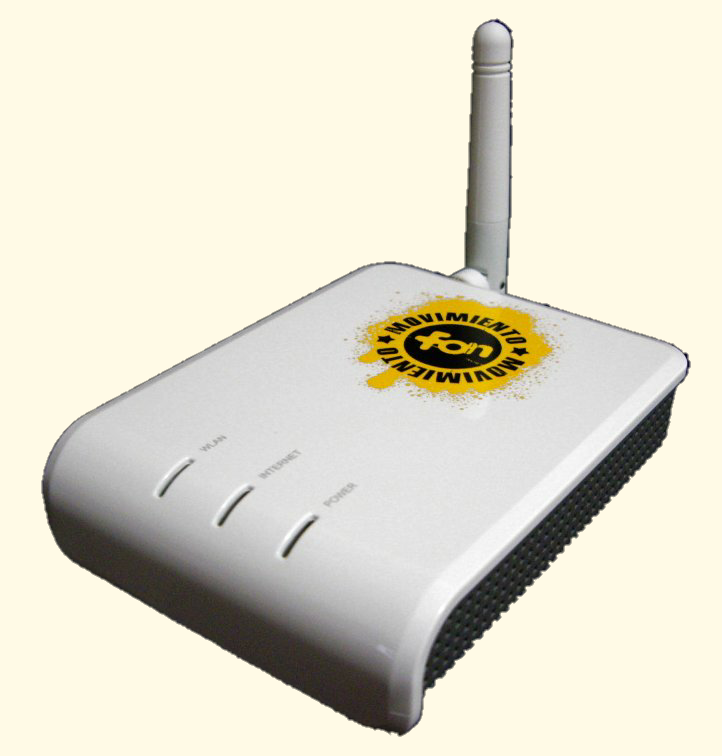
\includegraphics[keepaspectratio, width=0.2\textwidth]{images/lafonera-sourcewikipedia}
%  \caption{Figura 1. La Fonera}
%\end{figure}
\\
Figura 1. La Fonera. Fuente: Wikipedia.
\\
\end{center}
\section{Soluci\'on propuesta}\label{sec:solution}
(Por completar)
\subsection{Dise\~no} \label{ch:design}
(Por completar)
\subsubsection{Roles} \label{ch:roles}
(Por completar)
\\
\\
\textit{ETH-Paid hotspot provider} (E-Php).
\\
\\
\textit{Hotspot handler} (hh).
\\
\\
\textit{Upstream Internet Service Provider} (U-ISP).
\\
\\
Usuario.
\subsubsection{Arquitectura} \label{ch:architecture}
(Por completar)
\\
\\
Gesti\'on del stake.
\subsection{Implementaci\'on} \label{ch:implementation}
El estudio del equipamiento a utilizar es importante en cualquier proyecto. En esta secci\'on se har\'a una breve introducci\'on de los principales componentes con los que se ha trabajado. Tambi\'en se indicar\'a c\'omo se debe preparar la prueba de concepto (en adelante, PoC).
\subsubsection{Front-end} \label{ch:front-end}
(Por completar)
\subsubsection{Back-end} \label{ch:back-end}
(Por completar)
\\
\\
Raspberry Pi.
\\
\\
Se ha utilizado la Raspberry Pi 3 Modelo B (v\'ease figura 2). Un ordenador de placa reducida SBC (\textit{single board computer}).
\begin{center}
%\begin{figure}[h]
%  \centering
  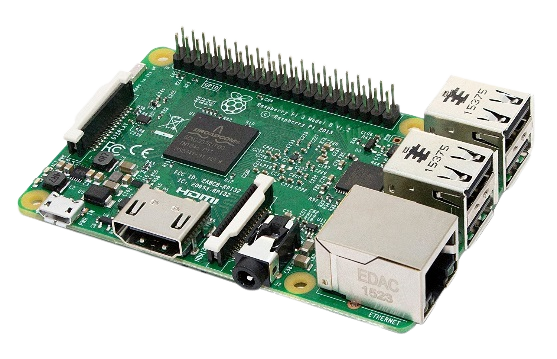
\includegraphics[keepaspectratio, width=0.2\textwidth]{images/rpi3modelb-sourceamazon.png}
%  \caption{Figura 2. Raspberry Pi 3 Modelo B. Fuente: [Raspberry 18]}
%\end{figure}
\\
Figura 2. Raspberry Pi 3 Modelo B. Fuente: [RaspberryPi 19]
\\
\end{center}
Un resumen de sus especificaciones se da a continuaci\'on (v\'ease tabla 1):
\begin{center}
%\begin{tabular} to 0.5\textwidth { | X[l] | X[r] | }
\begin{tabular}{ | m{0.125\textwidth} | m{0.3125\textwidth} | }
 \hline
 Especificaciones & Raspberry Pi 3 Modelo B \\
 \hline
 Procesador & Broadcom BCM2837, Cortex-A53 (ARMv8) 64-bit SoC @ 1,2 GHz \\
\hline
 RAM & 1 GB \\
\hline
 Conectividad & Wi-Fi 802.11 b/g/n (2,4 GHz) Bluetooth 4.1 Puerto Ethernet de hasta 100 Mbps \\
\hline
 Puertos & HDMI completo, 4 USB 2.0, MicroSD, CSI camera, DSI display \\
\hline
 Memoria & MicroSD \\
\hline
\end{tabular}
\newline
\end{center}
Tabla 1. Especificaciones de Raspberry Pi 3 Modelo B
%\newline
\\
\\
Aunque no se indica expresamente si es hardware libre (\textit{open hardware}) o con derechos de marca, en su p\'agina Web oficial explican que disponen de contratos de distribuci\'on y venta con dos empresas. Pero al mismo tiempo, cualquiera puede convertirse en revendedor o redistribuidor de las tarjetas Raspberry Pi [RaspberryPiBuy 19].
\\
\\
Smart contracts.
\\
\\
La parte smart contract consiste en un smart contract para pago con ETH y otro smart contract para pago con tokens.
\begin{itemize}
 \item Smart contract ETH
 \item Smart contract token
 \newline
\end{itemize}
(Por completar)
\section{Pruebas}\label{sec:proofs}
Para validar la PoC, se ha definido una bater\'\i{}a de tests. Por ejemplo, dado que los smart contract normalmente manejan dinero, es esencial asegurarse de que su n\'umero de fallos y vulnerabilidades sea bajo [Hegedus 18]. Para ayudar a los desarrolladores y hacer m\'as madura la tecnolog\'\i{}a, necesitamos herramientas de an\'alisis [ConsenSys 19].
\subsection{Tests} \label{ch:tests}
(Por completar)
\section{Viabilidad de negocio}\label{sec:business}
(Por completar)
\subsection{Legislaci\'on} \label{ch:legislation}
(Por completar)
\section{Conclusiones}\label{sec:conclusions}
El mundo en el que vivimos es interconectado. En \'el Internet juega un papel fundamental. Se ha contribuido a la construcci\'on de una PoC. \'Esta se ha basado en la medida de lo posible en hardware libre (Raspberry Pi) ya que goza de buena popularidad para el desarrollo de prototipos.

Como debilidad del pago con ETH, se puede achacar la volatilidad de su precio (v\'ease figura 3). Esto conlleva variaciones en las comisiones (\textit{fees}) de una transacci\'on Ethereum.
\begin{center}
%\begin{figure}[h]
%  \centering
  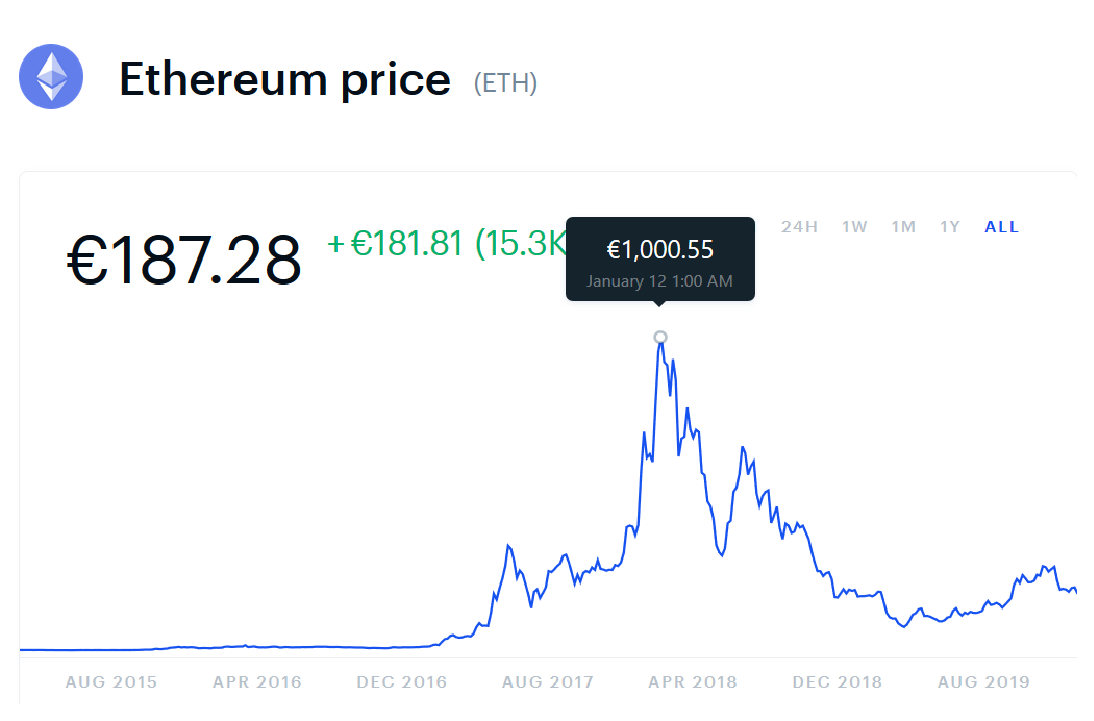
\includegraphics[keepaspectratio, width=0.481125\textwidth]{images/ethcurrentprice-sourcecoinbase}
%  \caption{Figura 3. Variación cotización ETH (11/08/2019)}
%\end{figure}
\\
Figura 3. Variaci\'on cotizaci\'on ETH (11/08/2019). Fuente: [Coinbase 19]
\\
\end{center}
(Por completar)
\section{L\'\i{}neas futuras}\label{sec:future}
Como l\'\i{}neas futuras y complemento a este trabajo, con m\'as tiempo, se plantea:
\subsection{A\~nadir forma de pago DAI} \label{ch:dai}
DAI es una criptomoneda estable (\textit{stablecoin}) que funciona con ETH y que intenta mantener un valor de 1\$. A diferencia de los billetes de banco centralizados, DAI no est\'a respaldado por d\'olares estadounidenses en una cuenta bancaria. En cambio, est\'a respaldado por garant\'\i{}as en la plataforma Maker [MakerDAO 19].
\section{Repositorio}\label{sec:repository}
(Por completar)
\\
\begin{center}
REFERENCIAS
\newline
\end{center}
[Coinbase 19] Coinbase. Intercambio de moneda digital. Disponible en: \href{https://www.coinbase.com/price/ethereum}{https://www.coinbase.com/price/ethereum}\newline\newline
[ConsenSys 19] Ethereum Smart Contract Best Practices. Security tools. ConsenSys. 12 Agosto 2019.\newline\newline
[Hegedus 18] P. Hegedus. "Towards Analyzing the Complexity Landscape of Solidity Based Ethereum Smart Contracts". 2018 IEEE/ACM 1st International Workshop on Emerging Trends in Software Engineering for Blockchain (WETSEB). 27 Mayo-3 Junio 2018. \href{https://ieeexplore.ieee.org/document/8445056}{https://ieeexplore.ieee.org/document/8445056}\newline\newline
[MakerDAO 19] MakerDAO. Stability for the blockchain. Disponible en: \href{https://makerdao.com/en/dai}{https://makerdao.com/en/dai}\newline\newline
[RaspberryPi 19] Raspberry Pi 3 Modelo B - Placa Base (1.2 GHz Quad-Core Arm Cortex-A53, 1 GB RAM, USB 2.0). Amazon. 11 Agosto 2019.\newline\newline
[RaspberryPiBuy 19] Raspberry Pi FAQs. BUYING AND SHIPPING. Where can I buy a Raspberry Pi?. P\'agina Web oficial. 11 Agosto 2019. Disponible en: \href{https://www.raspberrypi.org/help/faqs/#buyingWhere}{https://www.raspberrypi.org/help/faqs/\#buyingWhere}\newline\newline
[Stallings 04] W. Stallings. "Comunicaciones y redes de computadores". 1 Septiembre 2004. P\'aginas 904. Pearson Prentice Hall. ISBN-13: 978-8420541105.
\clearpage

\cite{buterin2013ethereum} first proposed the kernel of this work in late November, 2013. Though now evolved in many ways, the key functionality of a block-chain with a Turing-complete language and an effectively unlimited inter-transaction storage capability remains unchanged.

\cite{dwork92pricingvia} provided the first work into the usage of a cryptographic proof of computational expenditure (``proof-of-work'') as a means of transmitting a value signal over the Internet. The value-signal was utilised here as a spam deterrence mechanism rather than any kind of currency, but critically demonstrated the potential for a basic data channel to carry a \textit{strong economic signal}, allowing a receiver to make a physical assertion without having to rely upon \textit{trust}. \cite{back2002hashcash} later produced a system in a similar vein.

The first example of utilising the proof-of-work as a strong economic signal to secure a currency was by \cite{vishnumurthy03karma:a}. In this instance, the token was used to keep peer-to-peer file trading in check, providing ``consumers'' with the ability to make micro-payments to ``suppliers'' for their services. The security model afforded by the proof-of-work was augmented with digital signatures and a ledger in order to ensure that the historical record couldn't be corrupted and that malicious actors could not spoof payment or unjustly complain about service delivery. Five years later, \cite{nakamoto2008bitcoin} introduced another such proof-of-work-secured value token, somewhat wider in scope. The fruits of this project, Bitcoin, became the first widely adopted global decentralised transaction ledger.

Other projects built on Bitcoin's success; the alt-coins introduced numerous other currencies through alteration to the protocol. Some of the best known are Litecoin and Primecoin, discussed by \cite{sprankel2013technical}. Other projects sought to take the core value content mechanism of the protocol and repurpose it; \cite{aron2012bitcoin} discusses, for example, the Namecoin project which aims to provide a decentralised name-resolution system.

Other projects still aim to build upon the Bitcoin network itself, leveraging the large amount of value placed in the system and the vast amount of computation that goes into the consensus mechanism. The Mastercoin project, first proposed by \cite{mastercoin2013willett}, aims to build a richer protocol involving many additional high-level features on top of the Bitcoin protocol through utilisation of a number of auxiliary parts to the core protocol. The Coloured Coins project, proposed by \cite{colouredcoins2012rosenfeld}, takes a similar but more simplified strategy, embellishing the rules of a transaction in order to break the fungibility of Bitcoin's base currency and allow the creation and tracking of tokens through a special ``chroma-wallet''-protocol-aware piece of software.

Additional work has been done in the area with discarding the decentralisation foundation; Ripple, discussed by \cite{boutellier2014pirates}, has sought to create a ``federated'' system for currency exchange, effectively creating a new financial clearing system. It has demonstrated that high efficiency gains can be made if the decentralisation premise is discarded.

Early work on smart contracts has been done by \cite{szabo1997formalizing} and \cite{miller1997future}. Around the 1990s it became clear that algorithmic enforcement of agreements could become a significant force in human cooperation. Though no specific system was proposed to implement such a system, it was proposed that the future of law would be heavily affected by such systems. In this light, Ethereum may be seen as a general implementation of such a \textit{crypto-law} system.

%E language?
For a list of terms used in this paper, refer to Appendix \ref{ch:Terminology}.

\section{The Blockchain Paradigm} \label{ch:overview}

Ethereum, taken as a whole, can be viewed as a transaction-based state machine: we begin with a genesis state and incrementally execute transactions to morph it into some final state. It is this final state which we accept as the canonical ``version'' of the world of Ethereum. The state can include such information as account balances, reputations, trust arrangements, data pertaining to information of the physical world; in short, anything that can currently be represented by a computer is admissible. Transactions thus represent a valid arc between two states; the `valid' part is important---there exist far more invalid state changes than valid state changes. Invalid state changes might, \eg, be things such as reducing an account balance without an equal and opposite increase elsewhere. A valid state transition is one which comes about through a transaction. Formally:
\begin{equation}
\linkdest{Upsilon_state_transition}\linkdest{Upsilon}\boldsymbol{\sigma}_{t+1} \equiv \Upsilon(\boldsymbol{\sigma}_{t}, T)
\end{equation}

where $\Upsilon$ is the Ethereum state transition function. In Ethereum, $\Upsilon$, together with $\boldsymbol{\sigma}$ are considerably more powerful than any existing comparable system; $\Upsilon$ allows components to carry out arbitrary computation, while $\boldsymbol{\sigma}$ allows components to store arbitrary state between transactions.

Transactions are collated into blocks; blocks are chained together using a cryptographic hash as a means of reference. Blocks function as a journal, recording a series of transactions together with the previous block and an identifier for the final state (though do not store the final state itself---that would be far too big). They also punctuate the transaction series with incentives for nodes to \textit{mine}. This incentivisation takes place as a state-transition function, adding value to a nominated account.

Mining is the process of dedicating effort (working) to bolster one series of transactions (a block) over any other potential competitor block. It is achieved thanks to a cryptographically secure proof. This scheme is known as a proof-of-work and is discussed in detail in section \ref{ch:pow}.

Formally, we expand to:
\begin{eqnarray}
\boldsymbol{\sigma}_{t+1} & \equiv & \hyperlink{Pi}{\Pi}(\boldsymbol{\sigma}_{t}, B) \\
B & \equiv & (..., (T_0, T_1, ...), ...) \\
\Pi(\boldsymbol{\sigma}, B) & \equiv & \hyperlink{Omega}{\Omega}(B, \hyperlink{Upsilon}{\Upsilon}(\Upsilon(\boldsymbol{\sigma}, T_0), T_1) ...)
\end{eqnarray}

Where \hyperlink{Omega}{$\Omega$} is the block-finalisation state transition function (a function that rewards a nominated party); \hyperlink{block}{$B$} is this block, which includes a series of transactions amongst some other components; and $\hyperlink{Pi}{\Pi}$ is the block-level state-transition function.

This is the basis of the blockchain paradigm, a model that forms the backbone of not only Ethereum, but all decentralised consensus-based transaction systems to date.

\subsection{Value}

In order to incentivise computation within the network, there needs to be an agreed method for transmitting value. To address this issue, Ethereum has an intrinsic currency, Ether, known also as {\small ETH} and sometimes referred to by the Old English \DH{}. The smallest subdenomination of Ether, and thus the one in which all integer values of the currency are counted, is the Wei. One Ether is defined as being $10^{18}$ Wei. There exist other subdenominations of Ether:
\par
\begin{center}
\begin{tabular}{rl}
\toprule
Multiplier & Name \\
\midrule
$10^0$ & Wei \\
$10^{12}$ & Szabo \\
$10^{15}$ & Finney \\
$10^{18}$ & Ether \\
\bottomrule
\end{tabular}
\end{center}
\par

Throughout the present work, any reference to value, in the context of Ether, currency, a balance or a payment, should be assumed to be counted in Wei.

\subsection{Which History?}

Since the system is decentralised and all parties have an opportunity to create a new block on some older pre-existing block, the resultant structure is necessarily a tree of blocks. In order to form a consensus as to which path, from root (\hyperlink{Genesis_Block}{the genesis block}) to leaf (the block containing the most recent transactions) through this tree structure, known as the blockchain, there must be an agreed-upon scheme. If there is ever a disagreement between nodes as to which root-to-leaf path down the block tree is the `best' blockchain, then a \textit{fork} occurs.

This would mean that past a given point in time (block), multiple states of the system may coexist: some nodes believing one block to contain the canonical transactions, other nodes believing some other block to be canonical, potentially containing radically different or incompatible transactions. This is to be avoided at all costs as the uncertainty that would ensue would likely kill all confidence in the entire system.

The scheme we use in order to generate consensus is a simplified version of the GHOST protocol introduced by \cite{cryptoeprint:2013:881}. This process is described in detail in section \ref{ch:ghost}.

Sometimes, a path follows a new protocol from a particular height.  This document describes one version of the protocol.  In order to follow back the history of a path, one must reference multiple versions of this document.

\section{Conventions}\label{ch:conventions}

We use a number of typographical conventions for the formal notation, some of which are quite particular to the present work:

The two sets of highly structured, `top-level', state values, are denoted with bold lowercase Greek letters. They fall into those of world-state, which are denoted $\boldsymbol{\sigma}$ (or a variant thereupon) and those of machine-state, $\boldsymbol{\mu}$.

Functions operating on highly structured values are denoted with an upper-case Greek letter, \eg \hyperlink{Upsilon_state_transition}{$\Upsilon$}, the Ethereum state transition function.

For most functions, an uppercase letter is used, e.g. $C$, the general cost function. These may be subscripted to denote specialised variants, \eg \hyperlink{C__SSTORE}{$C_\text{SSTORE}$}, the cost function for the \hyperlink{SSTORE}{{\tiny SSTORE}} operation. For specialised and possibly externally defined functions, we may format as typewriter text, \eg the Keccak-256 hash function (as per version 3 of the winning entry to the SHA-3 contest by \cite{Keccak}, rather than the final SHA-3 specification), is denoted $\texttt{KEC}$ (and generally referred to as plain Keccak). Also, $\texttt{KEC512}$ refers to the Keccak-512 hash function.

Tuples are typically denoted with an upper-case letter, \eg $T$, is used to denote an Ethereum transaction. This symbol may, if accordingly defined, be subscripted to refer to an individual component, \eg \hyperlink{transaction_nonce}{$T_{\mathrm{n}}$}, denotes the nonce of said transaction. The form of the subscript is used to denote its type; \eg uppercase subscripts refer to tuples with subscriptable components.

Scalars and fixed-size byte sequences (or, synonymously, arrays) are denoted with a normal lower-case letter, \eg $n$ is used in the document to denote a \hyperlink{transaction_nonce}{transaction nonce}. Those with a particularly special meaning may be Greek, \eg $\delta$, the number of items required on the stack for a given operation.

Arbitrary-length sequences are typically denoted as a bold lower-case letter, \eg $\mathbf{o}$ is used to denote the byte sequence given as the output data of a message call. For particularly important values, a bold uppercase letter may be used.

Throughout, we assume scalars are non-negative integers and thus belong to the set $\mathbb{N}$. The set of all byte sequences is $\mathbb{B}$, formally defined in Appendix \ref{app:rlp}. If such a set of sequences is restricted to those of a particular length, it is denoted with a subscript, thus the set of all byte sequences of length $32$ is named $\mathbb{B}_{32}$ and the set of all non-negative integers smaller than $2^{256}$ is named $\mathbb{N}_{256}$. This is formally defined in section \hyperlink{block}{\ref{subsec:The_Block}}.

Square brackets are used to index into and reference individual components or subsequences of sequences, \eg $\boldsymbol{\mu}_{\mathbf{s}}[0]$ denotes the first item on the machine's stack. For subsequences, ellipses are used to specify the intended range, to include elements at both limits, \eg $\boldsymbol{\mu}_{\mathbf{m}}[0..31]$ denotes the first 32 items of the machine's memory.

In the case of the global state $\boldsymbol{\sigma}$, which is a sequence of accounts, themselves tuples, the square brackets are used to reference an individual account.

When considering variants of existing values, we follow the rule that within a given scope for definition, if we assume that the unmodified `input' value be denoted by the placeholder $\Box$ then the modified and utilisable value is denoted as $\Box'$, and intermediate values would be $\Box^*$,  $\Box^{**}$ \&c. On very particular occasions, in order to maximise readability and only if unambiguous in meaning, we may use alpha-numeric subscripts to denote intermediate values, especially those of particular note.

When considering the use of existing functions, given a function $f$, the function \hyperlink{general_element_wise_sequence_transformation_f_pow_asterisk}{$f^*$} denotes a similar, element-wise version of the function mapping instead between sequences. It is formally defined in section \hyperlink{block}{\ref{subsec:The_Block}}.

We define a number of useful functions throughout. \linkdest{ell}One of the more common is $\ell$, which evaluates to the last item in the given sequence:

\begin{equation}
\ell(\mathbf{x}) \equiv \mathbf{x}[\lVert \mathbf{x} \rVert - 1]
\end{equation}

\section{Blocks, State and Transactions} \label{ch:bst}

Having introduced the basic concepts behind Ethereum, we will discuss the meaning of a transaction, a block and the state in more detail.

\subsection{World State} \label{ch:state}

The world state (\textit{state}), is a mapping between addresses (160-bit identifiers) and account states (a data structure serialised as RLP, see Appendix \ref{app:rlp}). Though not stored on the blockchain, it is assumed that the implementation will maintain this mapping in a modified Merkle Patricia tree (\textit{trie}, see Appendix \ref{app:trie}). The trie requires a simple database backend that maintains a mapping of byte arrays to byte arrays; we name this underlying database the state database. This has a number of benefits; firstly the root node of this structure is cryptographically dependent on all internal data and as such its hash can be used as a secure identity for the entire system state. Secondly, being an immutable data structure, it allows any previous state (whose root hash is known) to be recalled by simply altering the root hash accordingly. Since we store all such root hashes in the blockchain, we are able to trivially revert to old states.

The account state, $\boldsymbol{\sigma}[a]$, comprises the following four fields:

\begin{description}
\item[nonce] \linkdest{account_nonce}A scalar value equal to the number of transactions sent from this address or, in the case of accounts with associated code, the number of contract-creations made by this account. For account of address $a$ in state $\boldsymbol{\sigma}$, this would be formally denoted $\boldsymbol{\sigma}[a]_{\mathrm{n}}$.
\item[balance] A scalar value equal to the number of Wei owned by this address. Formally denoted $\boldsymbol{\sigma}[a]_{\mathrm{b}}$.
\item[storageRoot] A 256-bit hash of the root node of a Merkle Patricia tree that encodes the storage contents of the account (a mapping between 256-bit integer values), encoded into the trie as a mapping from the Keccak 256-bit hash of the  256-bit integer keys to the RLP-encoded 256-bit integer values. The hash is formally denoted $\boldsymbol{\sigma}[a]_{\mathrm{s}}$.
\item[codeHash] The hash of the EVM code of this account---this is the code that gets executed should this address receive a message call; it is immutable and thus, unlike all other fields, cannot be changed after construction. All such code fragments are contained in the state database under their corresponding hashes for later retrieval. This hash is formally denoted $\boldsymbol{\sigma}[a]_{\mathrm{c}}$, and thus the code may be denoted as $\mathbf{b}$, given that $\texttt{KEC}(\mathbf{b}) = \boldsymbol{\sigma}[a]_{\mathrm{c}}$.
\end{description}

Since we typically wish to refer not to the trie's root hash but to the underlying set of key/value pairs stored within, we define a convenient equivalence:
\begin{equation}
\texttt{TRIE}\big(L_{I}^*(\boldsymbol{\sigma}[a]_{\mathbf{s}})\big) \equiv \boldsymbol{\sigma}[a]_{\mathrm{s}}
\end{equation}

The collapse function for the set of key/value pairs in the trie, $L_{I}^*$, is defined as the element-wise transformation of the base function $L_{I}$, given as:
\begin{equation}
L_{I}\big( (k, v) \big) \equiv \big(\texttt{KEC}(k), \texttt{RLP}(v)\big)
\end{equation}

where:
\begin{equation}
k \in \mathbb{B}_{32} \quad \wedge \quad v \in \mathbb{N}
\end{equation}

It shall be understood that $\boldsymbol{\sigma}[a]_{\mathbf{s}}$ is not a `physical' member of the account and does not contribute to its later serialisation.

If the \textbf{codeHash} field is the Keccak-256 hash of the empty string, i.e. $\boldsymbol{\sigma}[a]_{\mathrm{c}} = \texttt{KEC}\big(()\big)$, then the node represents a simple account, sometimes referred to as a ``non-contract'' account.

Thus we may define a world-state collapse function $L_{S}$:
\begin{equation}
L_{S}(\boldsymbol{\sigma}) \equiv \{ p(a): \boldsymbol{\sigma}[a] \neq \varnothing \}
\end{equation}
where
\begin{equation}
p(a) \equiv  \big(\texttt{KEC}(a), \texttt{RLP}\big( (\boldsymbol{\sigma}[a]_{\mathrm{n}}, \boldsymbol{\sigma}[a]_{\mathrm{b}}, \boldsymbol{\sigma}[a]_{\mathrm{s}}, \boldsymbol{\sigma}[a]_{\mathrm{c}}) \big) \big)
\end{equation}

This function, $L_{S}$, is used alongside the trie function to provide a short identity (hash) of the world state. We assume:
\begin{equation}
\forall a: \boldsymbol{\sigma}[a] = \varnothing \; \vee \; (a \in \mathbb{B}_{20} \; \wedge \; v(\boldsymbol{\sigma}[a]))
\end{equation}
\linkdest{account_validity_function_v__x}{}where $v$ is the account validity function:
\begin{equation}
\quad v(x) \equiv x_{\mathrm{n}} \in \mathbb{N}_{256} \wedge x_{\mathrm{b}} \in \mathbb{N}_{256} \wedge x_{\mathrm{s}} \in \mathbb{B}_{32} \wedge x_{\mathrm{c}} \in \mathbb{B}_{32}
\end{equation}

An account is \textit{empty} when it has no code, zero nonce and zero balance:
\begin{equation}
\mathtt{EMPTY}(\boldsymbol{\sigma}, a) \quad\equiv\quad \boldsymbol{\sigma}[a]_{\mathrm{c}} = \texttt{KEC}\big(()\big) \wedge \boldsymbol{\sigma}[a]_{\mathrm{n}} = 0 \wedge \boldsymbol{\sigma}[a]_{\mathrm{b}} = 0
\end{equation}
Even callable precompiled contracts can have an empty account state. This is because their account states do not usually contain the code describing its behavior.

An account is \textit{dead} when its account state is non-existent or empty:
\begin{equation}
\mathtt{DEAD}(\boldsymbol{\sigma}, a) \quad\equiv\quad \boldsymbol{\sigma}[a] = \varnothing \vee \mathtt{EMPTY}(\boldsymbol{\sigma}, a)
\end{equation}

\subsection{The Transaction} \label{subsec:transaction}

A transaction (formally, $T$) is a single cryptographically-signed instruction constructed by an actor externally to the scope of Ethereum. While it is assumed that the ultimate external actor will be human in nature, software tools will be used in its construction and dissemination\footnote{Notably, such `tools' could ultimately become so causally removed from their human-based initiation---or humans may become so causally-neutral---that there could be a point at which they rightly be considered autonomous agents. \eg contracts may offer bounties to humans for being sent transactions to initiate their execution.}. There are two types of transactions: those which result in message calls and those which result in the creation of new accounts with associated code (known informally as `contract creation'). Both types specify a number of common fields:

\begin{description}
\item[nonce]\linkdest{tx_nonce}{} A scalar value equal to the number of transactions sent by the sender; formally $T_{\mathrm{n}}$.
\item[gasPrice]\linkdest{tx_gas_price_T__p}{} A scalar value equal to the number of Wei to be paid per unit of \textit{gas} for all computation costs incurred as a result of the execution of this transaction; formally $T_{\mathrm{p}}$.
\item[gasLimit]\linkdest{tx_gas_limit_T__g}{} A scalar value equal to the maximum amount of gas that should be used in executing this transaction. This is paid up-front, before any computation is done and may not be increased later; formally $T_{\mathrm{g}}$.
\item[to]\linkdest{tx_to_address_T__t}{} The 160-bit address of the message call's recipient or, for a contract creation transaction, $\varnothing$, used here to denote the only member of $\mathbb{B}_0$ ; formally $T_{\mathrm{t}}$.
\item[value]\linkdest{tx_value_T__v}{} A scalar value equal to the number of Wei to be transferred to the message call's recipient or, in the case of contract creation, as an endowment to the newly created account; formally $T_{\mathrm{v}}$.
\item[v, r, s] Values corresponding to the signature of the transaction and used to determine the sender of the transaction; formally \linkdest{T__w_T__r_T__s}{$T_{\mathrm{w}}$, $T_{\mathrm{r}}$ and $T_{\mathrm{s}}$}. This is expanded in Appendix \ref{app:signing}.
\end{description}

Additionally, a contract creation transaction contains:

\begin{description}
\item[init] An unlimited size byte array specifying the EVM-code for the account initialisation procedure, formally $T_{\mathbf{i}}$.
\end{description}

\textbf{init} is an EVM-code fragment; it returns the \textbf{body}, a second fragment of code that executes each time the account receives a message call (either through a transaction or due to the internal execution of code). \textbf{init} is executed only once at account creation and gets discarded immediately thereafter.

In contrast, a message call transaction contains:

\begin{description}
\item[data] An unlimited size byte array specifying the input data of the message call, formally $T_{\mathbf{d}}$.
\end{description}

Appendix \ref{app:signing} specifies the function, $S$, which maps transactions to the sender, and happens through the ECDSA of the SECP-256k1 curve, using the hash of the transaction (excepting the latter three signature fields) as the datum to sign. For the present we simply assert that the sender of a given transaction $T$ can be represented with $S(T)$.

\begin{equation}
L_{T}(T) \equiv \begin{cases}
(T_{\mathrm{n}}, T_{\mathrm{p}}, T_{\mathrm{g}}, T_{\mathrm{t}}, T_{\mathrm{v}}, T_{\mathbf{i}}, T_{\mathrm{w}}, T_{\mathrm{r}}, T_{\mathrm{s}}) & \text{if} \; T_{\mathrm{t}} = \varnothing\\
(T_{\mathrm{n}}, T_{\mathrm{p}}, T_{\mathrm{g}}, T_{\mathrm{t}}, T_{\mathrm{v}}, T_{\mathbf{d}}, T_{\mathrm{w}}, T_{\mathrm{r}}, T_{\mathrm{s}}) & \text{otherwise}
\end{cases}
\end{equation}

Here, we assume all components are interpreted by the RLP as integer values, with the exception of the arbitrary length byte arrays $T_{\mathbf{i}}$ and $T_{\mathbf{d}}$.
\begin{equation}
\begin{array}[t]{lclclc}
T_{\mathrm{n}} \in \mathbb{N}_{256} & \wedge & T_{\mathrm{v}} \in \mathbb{N}_{256} & \wedge & T_{\mathrm{p}} \in \mathbb{N}_{256} & \wedge \\
T_{\mathrm{g}} \in \mathbb{N}_{256} & \wedge & T_{\mathrm{w}} \in \mathbb{N}_5 & \wedge & T_{\mathrm{r}} \in \mathbb{N}_{256} & \wedge \\
T_{\mathrm{s}} \in \mathbb{N}_{256} & \wedge & T_{\mathbf{d}} \in \mathbb{B} & \wedge & T_{\mathbf{i}} \in \mathbb{B}
\end{array}
\end{equation}
where
\begin{equation}
\mathbb{N}_{\mathrm{n}} = \{ P: P \in \mathbb{N} \wedge P < 2^n \}
\end{equation}

The address hash $T_{\mathbf{t}}$ is slightly different: it is either a 20-byte address hash or, in the case of being a contract-creation transaction (and thus formally equal to $\varnothing$), it is the RLP empty byte sequence and thus the member of $\mathbb{B}_0$:
\begin{equation}
T_{\mathbf{t}} \in \begin{cases} \mathbb{B}_{20} & \text{if} \quad T_{\mathrm{t}} \neq \varnothing \\
\mathbb{B}_{0} & \text{otherwise}\end{cases}
\end{equation}

\subsection{The Block}\linkdest{block}\label{subsec:The_Block}

The block in Ethereum is the collection of relevant pieces of information (known as the block \textit{header}), $H$, together with information corresponding to the comprised transactions, $\mathbf{T}$,\hypertarget{ommerheaders}{} and a set of other block headers $\mathbf{U}$ that are known to have a parent equal to the present block's parent's parent (such blocks are known as \textit{ommers}\footnote{\textit{ommer} is a gender-neutral term to mean ``sibling of parent''; see \url{https://nonbinary.miraheze.org/wiki/Gender_neutral_language\#Aunt.2FUncle}}). The block header contains several pieces of information:

%\textit{TODO: Introduce logs}

\begin{description}
\item[parentHash]\linkdest{parent_Hash_H__p_def_words}{} The Keccak 256-bit hash of the parent block's header, in its entirety; formally $H_{\mathrm{p}}$.
\item[ommersHash] The Keccak 256-bit hash of the ommers list portion of this block; formally $H_{\mathrm{o}}$.
\item[beneficiary]\linkdest{beneficiary_H__c}{}\linkdest{H__c} The 160-bit address to which all fees collected from the successful mining of this block be transferred; formally $H_{\mathrm{c}}$.
\item[stateRoot] The Keccak 256-bit hash of the root node of the state trie, after all transactions are executed and finalisations applied; formally $H_{\mathrm{r}}$.
\item[transactionsRoot] The Keccak 256-bit hash of the root node of the trie structure populated with each transaction in the transactions list portion of the block; formally $H_{\mathrm{t}}$.
\item[receiptsRoot]\linkdest{receipts_Root_def_words}{} The Keccak 256-bit hash of the root node of the trie structure populated with the receipts of each transaction in the transactions list portion of the block; formally $H_{\mathrm{e}}$.
\item[logsBloom]\linkdest{logs_Bloom_def_words}{} The Bloom filter composed from indexable information (logger address and log topics) contained in each log entry from the receipt of each transaction in the transactions list; formally $H_{\mathrm{b}}$.
\item[difficulty] A scalar value corresponding to the difficulty level of this block. This can be calculated from the previous block's difficulty level and the timestamp; formally $H_{\mathrm{d}}$.
\item[number]\linkdest{block_number_word_def_H_i}{} A scalar value equal to the number of ancestor blocks. The genesis block has a number of zero; formally \hyperlink{block_number_H__i}{$H_{\mathrm{i}}$}.
\item[gasLimit] A scalar value equal to the current limit of gas expenditure per block; formally $H_{\mathrm{l}}$.
\item[gasUsed]\linkdest{block_gas_used_H__g}{}\linkdest{H__g} A scalar value equal to the total gas used in transactions in this block; formally $H_{\mathrm{g}}$.
\item[timestamp]\linkdest{block_timestamp_word_def_H__s}{} A scalar value equal to the reasonable output of Unix's time() at this block's inception; formally \hyperlink{block_timestamp_H__s}{$H_{\mathrm{s}}$}.
\item[extraData]\linkdest{block_extraData_H__x}{} An arbitrary byte array containing data relevant to this block. This must be 32 bytes or fewer; formally $H_{\mathrm{x}}$.
\item[mixHash]\linkdest{mixHash_H__m}{}\linkdest{H__m} A 256-bit hash which, combined with the nonce, proves that a sufficient amount of computation has been carried out on this block; formally $H_{\mathrm{m}}$.
\item[nonce]\linkdest{block_nonce_H__n}{}\linkdest{block_nonce} A 64-bit value which, combined with the mix-hash, proves that a sufficient amount of computation has been carried out on this block; formally \hyperlink{H__n}{$H_{\mathrm{n}}$}.
\end{description}
\linkdest{ommer_block_headers_B__U}{}\linkdest{block_B}{}The other two components in the block are simply a list of ommer block headers (of the same format as above), $B_{\mathbf{U}}$ and a series of the transactions, $B_{\mathbf{T}}$. Formally, we can refer to a block $B$:
\begin{equation}
B \equiv (B_{H}, B_{\mathbf{T}}, B_{\mathbf{U}})
\end{equation}

\subsubsection{Transaction Receipt}\linkdest{Transaction_Receipt}{}

In order to encode information about a transaction concerning which it may be useful to form a zero-knowledge proof, or index and search, we encode a receipt of each transaction containing certain information from its execution.
Each receipt, denoted $B_{\mathbf{R}}[i]$ for the $i$th transaction, is placed in an index-keyed \hyperlink{trie}{trie} and the root recorded in the header as \hyperlink{Receipts_Root_H__e}{$H_{\mathrm{e}}$}.

\linkdest{transaction_receipt_R}{}\linkdest{tx_receipt_gas_used_R__u}{}\linkdest{R__u}The transaction receipt, $R$, is a tuple of four items comprising: the cumulative gas used in the block containing the transaction receipt as of immediately after the transaction has happened, $R_{\mathrm{u}}$, the set of logs created through execution of the transaction, \hyperlink{RLP_serialisation_of_a_sequence_of_other_items_R__l_math_def}{$R_\mathbf{l}$} and the Bloom filter composed from information in those logs, \hyperlink{RLP_serialisation_of_a_byte_array_R__b_math_def}{$R_{\mathrm{b}}$} and the status code of the transaction, $R_{\mathrm{z}}$:
\begin{equation}
R \equiv (R_{\mathrm{u}}, R_{\mathrm{b}}, R_{\mathbf{l}}, R_{\mathrm{z}})
\end{equation}

\hypertarget{transaction_receipt_preparation_function_for_RLP_serialisation}{}\linkdest{L__R}The function $L_{R}$ trivially prepares a transaction receipt for being transformed into an RLP-serialised byte array:
\begin{equation}
L_{R}(R) \equiv (0 \in \mathbb{B}_{256}, R_{\mathrm{u}}, R_{\mathrm{b}}, R_{\mathbf{l}})
\end{equation}
where $0 \in \mathbb{B}_{256}$ replaces the pre-transaction state root that existed in previous versions of the protocol.

\linkdest{R__z_assert}We assert that the status code $R_{\mathrm{z}}$ is a non-negative integer.
\begin{equation}
R_{\mathrm{z}} \in \mathbb{N}
\end{equation}

\linkdest{R__u_assert}We assert that $R_{\mathrm{u}}$, the cumulative gas used, is a non-negative integer and that the logs Bloom, $R_{\mathrm{b}}$, is a hash of size 2048 bits (256 bytes):
\begin{equation}
R_{\mathrm{u}} \in \mathbb{N} \quad \wedge \quad R_{\mathrm{b}} \in \mathbb{B}_{256}
\end{equation}

%Notably $B_{\mathbf{T}}$ does not get serialised into the block by the block preparation function $L_{B}$; it is merely a convenience equivalence.

The sequence $R_{\mathbf{l}}$ is a series of log entries, $(O_0, O_1, ...)$. A log entry, $O$, is a tuple of the logger's address, $O_a$, a possibly empty series of 32-byte log topics, $O_{\mathbf{t}}$ and some number of bytes of data, $O_{\mathbf{d}}$:
\begin{equation}
O \equiv (O_{\mathrm{a}}, ({O_{\mathbf{t}}}_0, {O_{\mathbf{t}}}_1, ...), O_{\mathbf{d}})
\end{equation}
\begin{equation}
O_{\mathrm{a}} \in \mathbb{B}_{20} \quad \wedge \quad \forall x \in O_{\mathbf{t}}: x \in \mathbb{B}_{32} \quad \wedge \quad O_{\mathbf{d}} \in \mathbb{B}
\end{equation}

We define the Bloom filter function, $M$, to reduce a log entry into a single 256-byte hash:
\begin{equation}
M(O) \equiv \hyperlink{bigvee}{\bigvee}_{x \in \{O_{\mathrm{a}}\} \cup O_{\mathbf{t}}} \big( M_{3:2048}(x) \big)
\end{equation}

where $M_{3:2048}$ is a specialised Bloom filter that sets three bits out of 2048, given an arbitrary byte sequence. It does this through taking the low-order 11 bits of each of the first three pairs of bytes in a Keccak-256 hash of the byte sequence.\footnote{11 bits $= 2^{2048}$, and the low-order 11 bits is the modulo 2048 of the operand, which is in this case is "each of the first three pairs of bytes in a Keccak-256 hash of the byte sequence."} Formally:
\begin{eqnarray}
M_{3:2048}(\mathbf{x}: \mathbf{x} \in \mathbb{B}) & \equiv & \mathbf{y}: \mathbf{y} \in \mathbb{B}_{256} \quad \text{where:}\\
\mathbf{y} & = & (0, 0, ..., 0) \quad \text{except:}\\
\forall i \in \{0, 2, 4\}&:&\mathcal{B}_{m(\mathbf{x}, i)}(\mathbf{y}) = 1\\
m(\mathbf{x}, i) &\equiv& \mathtt{KEC}(\mathbf{x})[i, i + 1] \bmod 2048
\end{eqnarray}

where $\mathcal{B}$ is the bit reference function such that $\mathcal{B}_{\mathrm{j}}(\mathbf{x})$ equals the bit of index $j$ (indexed from 0) in the byte array $\mathbf{x}$.

\subsubsection{Holistic Validity}

\linkdest{block_validity}{}We can assert a block's validity if and only if it satisfies several conditions: it must be internally consistent with the ommer and transaction block hashes and the given transactions $B_{\mathbf{T}}$ (as specified in sec \ref{ch:finalisation}), when executed in order on the base state $\boldsymbol{\sigma}$ (derived from the final state of the parent block), result in a new state of the identity $H_{\mathrm{r}}$:
\begin{equation}
\begin{array}[t]{lclc}
\linkdest{new_state_H__r}{}H_{\mathrm{r}} &\equiv& \mathtt{TRIE}(L_S(\Pi(\boldsymbol{\sigma}, B))) & \wedge \\
\linkdest{Ommer_block_hash_H__o}{}H_{\mathrm{o}} &\equiv& \mathtt{KEC}(\mathtt{RLP}(L_H^*(B_{\mathbf{U}}))) & \wedge \\
\linkdest{tx_block_hash_H__t}{}H_{\mathrm{t}} &\equiv& \mathtt{TRIE}(\{\forall i < \lVert B_{\mathbf{T}} \rVert, i \in \mathbb{N}: &\\&& \quad\quad p (i, L_{T}(B_{\mathbf{T}}[i]))\}) & \wedge \\
\linkdest{Receipts_Root_H__e}{}H_{\mathrm{e}} &\equiv& \mathtt{TRIE}(\{\forall i < \lVert B_{\mathbf{R}} \rVert, i \in \mathbb{N}: &\\&& \quad\quad p(i, \hyperlink{transaction_receipt_preparation_function_for_RLP_serialisation}{L_{R}}(B_{\mathbf{R}}[i]))\}) & \wedge \\
\linkdest{logs_Bloom_filter_H__b}{}H_{\mathrm{b}} &\equiv& \bigvee_{\mathbf{r} \in B_{\mathbf{R}}} \big( \mathbf{r}_{\mathrm{b}} \big)
\end{array}
\end{equation}
where $p(k, v)$ is simply the pairwise RLP transformation, in this case, the first being the index of the transaction in the block and the second being the transaction receipt:
\begin{equation}
p(k, v) \equiv \big( \mathtt{RLP}(k), \mathtt{RLP}(v) \big)
\end{equation}

Furthermore:
\begin{equation}
\mathtt{TRIE}(L_{S}(\boldsymbol{\sigma})) = {P(B_H)_H}_{\mathrm{r}}
\end{equation}

Thus $\texttt{TRIE}(L_{S}(\boldsymbol{\sigma}))$ is the root node hash of the Merkle Patricia tree structure containing the key-value pairs of the state $\boldsymbol{\sigma}$ with values encoded using RLP, and $P(B_{H})$ is the parent block of $B$, defined directly.

The values stemming from the computation of transactions, specifically the \hyperlink{Transaction_Receipt}{transaction receipts}, $B_{\mathbf{R}}$, and that defined through the transaction's \hyperlink{Pi}{state-accumulation function, $\Pi$}, are formalised later in section \ref{sec:statenoncevalidation}.

\subsubsection{Serialisation}

\hypertarget{block_preparation_function_for_RLP_serialization_L__B}{}\linkdest{L__B}\hypertarget{block_preparation_function_for_RLP_serialization_L__H}{}\linkdest{L__B}The function $L_{B}$ and $L_{H}$ are the preparation functions for a block and block header respectively. Much like the \hyperlink{transaction_receipt_preparation_function_for_RLP_serialisation}{transaction receipt preparation function $L_{R}$}, we assert the types and order of the structure for when the RLP transformation is required:
\begin{eqnarray}
\quad L_{H}(H) & \equiv & (\begin{array}[t]{l}H_{\mathrm{p}}, H_{\mathrm{o}}, H_{\mathrm{c}}, H_{\mathrm{r}}, H_{\mathrm{t}}, H_{\mathrm{e}}, H_{\mathrm{b}}, H_{\mathrm{d}},\\ H_{\mathrm{i}}, H_{\mathrm{l}}, H_{\mathrm{g}}, H_{\mathrm{s}}, H_{\mathrm{x}}, H_{\mathrm{m}}, H_{\mathrm{n}} \; )\end{array} \\
\quad L_{B}(B) & \equiv & \big( L_{H}(B_{H}), L_{T}^*(B_{\mathbf{T}}), L_{H}^*(\hyperlink{ommer_block_headers_B__U}{B_{\mathbf{U}}}) \big)
\end{eqnarray}

\hypertarget{general_element_wise_sequence_transformation_f_pow_asterisk}{}With $L_T^*$ and $L_H^*$ being element-wise sequence transformations, thus:
\begin{equation}
\hyperlink{general_element_wise_sequence_transformation_f_pow_asterisk}{f^*}\big( (x_0, x_1, ...) \big) \equiv \big( f(x_0), f(x_1), ... \big) \quad \text{for any function} \; f
\end{equation}

The component types are defined thus:
\begin{equation}
\begin{array}[t]{lclclcl}
\hyperlink{parent_Hash_H__p_def_words}{H_{\mathrm{p}}} \in \mathbb{B}_{32} & \wedge & H_{\mathrm{o}} \in \mathbb{B}_{32} & \wedge & H_{\mathrm{c}} \in \mathbb{B}_{20} & \wedge \\
\hyperlink{new_state_H__r}{H_{\mathrm{r}}} \in \mathbb{B}_{32} & \wedge & H_{\mathrm{t}} \in \mathbb{B}_{32} & \wedge & \hyperlink{Receipts_Root_H__e}{H_{\mathrm{e}}} \in \mathbb{B}_{32} & \wedge \\
\hyperlink{logs_Bloom_filter_H__b}{H_{\mathrm{b}}} \in \mathbb{B}_{256} & \wedge & H_{\mathrm{d}} \in \mathbb{N} & \wedge & \hyperlink{block_number_H__i}{H_{\mathrm{i}}} \in \mathbb{N} & \wedge \\
\hyperlink{block_gas_limit_H__l}{H_{\mathrm{l}}} \in \mathbb{N} & \wedge & H_{\mathrm{g}} \in \mathbb{N} & \wedge & \hyperlink{block_timestamp_H__s}{H_{\mathrm{s}}} \in \mathbb{N}_{256} & \wedge \\
\hyperlink{block_extraData_H__x}{H_{\mathrm{x}}} \in \mathbb{B} & \wedge & H_{\mathrm{m}} \in \mathbb{B}_{32} & \wedge & \hyperlink{block_nonce_H__n}{H_{\mathrm{n}}} \in \mathbb{B}_{8}
\end{array}
\end{equation}

where
\begin{equation}
\mathbb{B}_{\mathrm{n}} = \{ B: B \in \mathbb{B} \wedge \lVert B \rVert = n \}
\end{equation}

We now have a rigorous specification for the construction of a formal block structure. The RLP function $\texttt{RLP}$ (see Appendix \ref{app:rlp}) provides the canonical method for transforming this structure into a sequence of bytes ready for transmission over the wire or storage locally.

\subsubsection{Block Header Validity}

We define $P(B_{H})$ to be the parent block of $B$, formally:
\begin{equation}
P(H) \equiv B': \mathtt{KEC}(\mathtt{RLP}(B'_{H})) = \hyperlink{parent_Hash_H__p_def_words}{H_{\mathrm{p}}}
\end{equation}

\hypertarget{block_number_H__i}{}The block number is the parent's block number incremented by one:
\begin{equation}
H_{\mathrm{i}} \equiv {{P(H)_{H}}_{\mathrm{i}}} + 1
\end{equation}

\newcommand{\mindifficulty}{D_0}
\newcommand{\homesteadmod}{\ensuremath{\varsigma_2}}
\newcommand{\expdiffsymb}{\ensuremath{\epsilon}}
\newcommand{\diffadjustment}{x}

\hypertarget{block_difficulty_H__d}{}\linkdest{H__d}The canonical difficulty of a block of header $H$ is defined as $D(H)$:
\begin{equation}
D(H) \equiv \begin{dcases}
\mindifficulty & \text{if} \quad H_{\mathrm{i}} = 0\\
\text{max}\!\left(\mindifficulty, {P(H)_{H}}_{\mathrm{d}} + \diffadjustment\times\homesteadmod + \expdiffsymb \right) & \text{otherwise}\\
\end{dcases}
\end{equation}
where:
\begin{equation}
\mindifficulty \equiv 131072
\end{equation}
\begin{equation}
\diffadjustment \equiv \left\lfloor\frac{{P(H)_{H}}_{\mathrm{d}}}{2048}\right\rfloor
\end{equation}
\begin{equation}
\homesteadmod \equiv \text{max}\left( y - \left\lfloor\frac{H_{\mathrm{s}} - {P(H)_{H}}_{\mathrm{s}}}{9}\right\rfloor, -99 \right)
\end{equation}
\begin{equation*}
y \equiv \begin{cases}
1 & \text{if} \, \lVert P(H)_{\mathbf{U}}\rVert = 0 \\
2 & \text{otherwise}
\end{cases}
\end{equation*}
\begin{align}
\expdiffsymb &\equiv \left\lfloor 2^{ \left\lfloor H'_{\mathrm{i}} \div 100000 \right\rfloor - 2 } \right\rfloor \\
H'_{\mathrm{i}} &\equiv \max(H_{\mathrm{i}} - 3000000, 0)
\end{align}

Note that $\mindifficulty$ is the difficulty of the genesis block. The \textit{Homestead} difficulty parameter, $\homesteadmod$, is used to affect a dynamic homeostasis of time between blocks, as the time between blocks varies, as discussed below, as implemented in EIP-2 by \cite{EIP-2}. In the Homestead release, the exponential difficulty symbol, $\expdiffsymb$ causes the difficulty to slowly increase (every 100,000 blocks) at an exponential rate, and thus increasing the block time difference, and putting time pressure on transitioning to proof-of-stake. This effect, known as the "difficulty bomb", or "ice age", was explained in EIP-649 by \cite{EIP-649} and delayed and implemented earlier in EIP-2. $\homesteadmod$ was also modified in EIP-100 with the use of $x$, the adjustment factor above, and the denominator 9, in order to target the mean block time including uncle blocks by \cite{EIP-100}. Finally, in the Byzantium release, with EIP-649, the ice age was delayed by creating a fake block number, $H'_{\mathrm{i}}$, which is obtained by subtracting three million from the actual block number, which in other words reduced $\expdiffsymb$ and the time difference between blocks, in order to allow more time to develop proof-of-stake and preventing the network from "freezing" up.

\hypertarget{block_gas_limit_H__l}{}The canonical gas limit $H_{\mathrm{l}}$ of a block of header $H$ must fulfil the relation:
\begin{eqnarray}
& & H_{\mathrm{l}} < {P(H)_{H}}_{\mathrm{l}} + \left\lfloor\frac{{P(H)_{H}}_{\mathrm{l}}}{1024}\right\rfloor \quad \wedge \\
\nonumber& & H_{\mathrm{l}} > {P(H)_{H}}_{\mathrm{l}} - \left\lfloor\frac{{P(H)_{H}}_{\mathrm{l}}}{1024}\right\rfloor \quad \wedge \\
\nonumber& & H_{\mathrm{l}} \geqslant 5000
\end{eqnarray}

\hypertarget{block_timestamp_H__s}{}$H_{\mathrm{s}}$ is the timestamp (in Unix's time()) of block $H$ and must fulfil the relation:
\begin{equation}
H_{\mathrm{s}} > {P(H)_{H}}_{\mathrm{s}}
\end{equation}

This mechanism enforces a homeostasis in terms of the time between blocks; a smaller period between the last two blocks results in an increase in the difficulty level and thus additional computation required, lengthening the likely next period. Conversely, if the period is too large, the difficulty, and expected time to the next block, is reduced.

The nonce, \linkdest{H__n}\hyperlink{block_nonce_H__n}{$H_{\mathrm{n}}$}, must satisfy the relations:
\begin{equation}
n \leqslant \frac{2^{256}}{H_{\mathrm{d}}} \quad \wedge \quad m = H_{\mathrm{m}}
\end{equation}
with $(n, m) = \mathtt{PoW}(H_{\hcancel{n}}, H_{\mathrm{n}}, \mathbf{d})$.

\hypertarget{block_header_without_nonce_and_mixmash_h__cancel_n}{}\linkdest{H_cancel_n}Where $H_{\hcancel{n}}$ is the new block's header $H$, but \textit{without} the nonce and mix-hash components, $\mathbf{d}$ being the current DAG, a large data set needed to compute the mix-hash, and $\mathtt{PoW}$ is the proof-of-work function (see section \ref{ch:pow}): this evaluates to an array with the first item being the mix-hash, to prove that a correct DAG has been used, and the second item being a pseudo-random number cryptographically dependent on $H$ and $\mathbf{d}$. Given an approximately uniform distribution in the range $[0, 2^{64})$, the expected time to find a solution is proportional to the difficulty, $H_{\mathrm{d}}$.

This is the foundation of the security of the blockchain and is the fundamental reason why a malicious node cannot propagate newly created blocks that would otherwise overwrite (``rewrite'') history. Because the nonce must satisfy this requirement, and because its satisfaction depends on the contents of the block and in turn its composed transactions, creating new, valid, blocks is difficult and, over time, requires approximately the total compute power of the trustworthy portion of the mining peers.

\hypertarget{block_header_validity_function}{}Thus we are able to define the block header validity function $V(H)$:
\begin{eqnarray}
V(H) & \equiv &  n \leqslant \frac{2^{256}}{H_{\mathrm{d}}} \wedge m = H_{\mathrm{m}} \quad \wedge \\
\nonumber & & H_{\mathrm{d}} = D(H) \quad \wedge \\
\nonumber& & H_{\mathrm{g}} \le H_{\mathrm{l}}  \quad \wedge \\
\nonumber& & H_{\mathrm{l}} < {P(H)_{H}}_{\mathrm{l}} + \left\lfloor\frac{{P(H)_{H}}_{\mathrm{l}}}{1024}\right\rfloor  \quad \wedge \\
\nonumber& & H_{\mathrm{l}} > {P(H)_{H}}_{\mathrm{l}} - \left\lfloor\frac{{P(H)_{H}}_{\mathrm{l}}}{1024}\right\rfloor  \quad \wedge \\
\nonumber& & H_{\mathrm{l}} \geqslant 5000  \quad \wedge \\
\nonumber& & H_{\mathrm{s}} > {P(H)_{H}}_{\mathrm{s}} \quad \wedge \\
\nonumber& & H_{\mathrm{i}} = {P(H)_{H}}_{\mathrm{i}} +1 \quad \wedge \\
\nonumber& & \lVert H_{\mathrm{x}} \rVert \le 32
\end{eqnarray}
where $(n, m) = \mathtt{PoW}(H_{\hcancel{n}}, H_{\mathrm{n}}, \mathbf{d})$

Noting additionally that \textbf{extraData} must be at most 32 bytes.

\section{Gas and Payment} \label{ch:payment}

In order to avoid issues of network abuse and to sidestep the inevitable questions stemming from Turing completeness, all programmable computation in Ethereum is subject to fees. The fee schedule is specified in units of \textit{gas} (see Appendix \ref{app:fees} for the fees associated with various computation). Thus any given fragment of programmable computation (this includes creating contracts, making message calls, utilising and accessing account storage and executing operations on the virtual machine) has a universally agreed cost in terms of gas.

Every transaction has a specific amount of gas associated with it: \textbf{gasLimit}. This is the amount of gas which is implicitly purchased from the sender's account balance. The purchase happens at the according \textbf{gasPrice}, also specified in the transaction. The transaction is considered invalid if the account balance cannot support such a purchase. It is named \textbf{gasLimit} since any unused gas at the end of the transaction is refunded (at the same rate of purchase) to the sender's account. Gas does not exist outside of the execution of a transaction. Thus for accounts with trusted code associated, a relatively high gas limit may be set and left alone.

In general, Ether used to purchase gas that is not refunded is delivered to the \textit{beneficiary} address, the address of an account typically under the control of the miner. Transactors are free to specify any \textbf{gasPrice} that they wish, however miners are free to ignore transactions as they choose. A higher gas price on a transaction will therefore cost the sender more in terms of Ether and deliver a greater value to the miner and thus will more likely be selected for inclusion by more miners. Miners, in general, will choose to advertise the minimum gas price for which they will execute transactions and transactors will be free to canvas these prices in determining what gas price to offer. Since there will be a (weighted) distribution of minimum acceptable gas prices, transactors will necessarily have a trade-off to make between lowering the gas price and maximising the chance that their transaction will be mined in a timely manner.

%\subsubsection{Determining Computation Costs}

\section{Transaction Execution} \label{ch:transactions}

The execution of a transaction is the most complex part of the Ethereum protocol: it defines the state transition function \hyperlink{Upsilon_state_transition}{$\Upsilon$}. It is assumed that any transactions executed first pass the initial tests of intrinsic validity. These include:

\begin{enumerate}
\item The transaction is well-formed RLP, with no additional trailing bytes;
\item the transaction signature is valid;
\item the \hyperlink{transaction_nonce}{transaction nonce} is valid (equivalent to the \hyperlink{account_nonce}{sender account's current nonce});
\item the gas limit is no smaller than the intrinsic gas, $g_0$, used by the transaction; and
\item the sender account balance contains at least the cost, $v_0$, required in up-front payment.
\end{enumerate}

Formally, we consider the function \hyperlink{Upsilon_state_transition}{$\Upsilon$}, with $T$ being a transaction and $\boldsymbol{\sigma}$ the state:
\begin{equation}
\boldsymbol{\sigma}' = \Upsilon(\boldsymbol{\sigma}, T)
\end{equation}

Thus $\boldsymbol{\sigma}'$ is the post-transactional state. We also define \hyperlink{tx_total_gas_used_Upsilon_pow_g}{$\Upsilon^{\mathrm{g}}$} to evaluate to the amount of gas used in the execution of a transaction, \hyperlink{tx_logs_Upsilon_pow_l}{$\Upsilon^{\mathbf{l}}$} to evaluate to the transaction's accrued log items and \hyperlink{tx_status_Upsilon_pow_z}{$\Upsilon^{\mathrm{z}}$} to evaluate to the status code resulting from the transaction. These will be formally defined later.

\subsection{Substate}
Throughout transaction execution, we accrue certain information that is acted upon immediately following the transaction. We call this the \textit{accrued transaction substate}, or \textit{accrued substate} for short, and represent it as $A$, which is a tuple:
\begin{equation}
A \equiv (A_{\mathbf{s}}, A_{\mathbf{l}}, A_{\mathbf{t}}, A_{\mathrm{r}})
\end{equation}

\hypertarget{self_destruct_set_wordy_defn_A__s}{}The tuple contents include $A_{\mathbf{s}}$, the self-destruct set: a set of accounts that will be discarded following the transaction's completion.\hypertarget{tx_log_series_wordy_defn_A__l}{} $A_{\mathbf{l}}$ is the log series: this is a series of archived and indexable `checkpoints' in VM code execution that allow for contract-calls to be easily tracked by onlookers external to the Ethereum world (such as decentralised application front-ends).\hypertarget{tx_touched_accounts_wordy_defn_A__t}{} $A_{\mathbf{t}}$ is the set of touched accounts, of which the empty ones are deleted at the end of a transaction.\hypertarget{refund_balance_defn_words_A__r}{} Finally there is $A_{\mathrm{r}}$, the refund balance, increased through using the \hyperlink{SSTORE}{{\small SSTORE}} instruction in order to reset contract storage to zero from some non-zero value. Though not immediately refunded, it is allowed to partially offset the total execution costs.

We define the empty accrued substate $A^0$ to have no self-destructs, no logs, no touched accounts and a zero refund balance:
\begin{equation}
A^0 \equiv (\varnothing,(), \varnothing, 0)
\end{equation}

\subsection{Execution}
\hypertarget{intrinsic_gas_g_0}{}We define intrinsic gas $g_0$, the amount of gas this transaction requires to be paid prior to execution, as follows:
\begin{align}
g_0 \equiv {} & \sum_{i \in T_{\mathbf{i}}, T_{\mathbf{d}}} \begin{cases} \hyperlink{G__txdatazero}{G_{\mathrm{txdatazero}}} & \text{if} \quad i = 0 \\ \hyperlink{G__txdatanonzero}{G_{\mathrm{txdatanonzero}}} & \text{otherwise} \end{cases} \\
{} & + \begin{cases} \hyperlink{G__txcreate}{G_{\mathrm{txcreate}}} & \text{if} \quad T_{\mathrm{t}} = \varnothing \\ 0 & \text{otherwise} \end{cases} \\
{} & + \hyperlink{G__transaction}{G_{\mathrm{transaction}}}
\end{align}

where $T_{\mathbf{i}},T_{\mathbf{d}}$ means the series of bytes of the transaction's associated data and initialisation EVM-code, depending on whether the transaction is for contract-creation or message-call. $G_{\mathrm{txcreate}}$ is added if the transaction is contract-creating, but not if a result of EVM-code. $G$ is fully defined in Appendix \ref{app:fees}.

The up-front cost $v_0$ is calculated as:
\begin{equation}
v_0 \equiv \hyperlink{tx_gas_limit_T__g}{T_{\mathrm{g}}} \hyperlink{tx_gas_price_T__p}{T_{\mathrm{p}}} + \hyperlink{tx_value_T__v}{T_{\mathrm{v}}}
\end{equation}

The validity is determined as:
\begin{equation}
\begin{array}[t]{rcl}
S(T) & \neq & \varnothing \quad \wedge \\
\boldsymbol{\sigma}[S(T)] & \neq & \varnothing \quad \wedge \\
\linkdest{transaction_nonce}{}T_{\mathrm{n}} & = & \boldsymbol{\sigma}[S(T)]_{\mathrm{n}} \quad \wedge \\
g_0 & \leqslant & T_{\mathrm{g}} \quad \wedge \\
v_0 & \leqslant & \boldsymbol{\sigma}[S(T)]_{\mathrm{b}} \quad \wedge \\
T_{\mathrm{g}} & \leqslant & {B_{H}}_{\mathrm{l}} - \hyperlink{ell}{\ell}(B_{\mathbf{R}})_{\mathrm{u}}
\end{array}
\end{equation}

Note the final condition; the sum of the transaction's gas limit, $T_{\mathrm{g}}$, and the gas utilised in this block prior, given by $\hyperlink{ell}{\ell}(B_{\mathbf{R}})_{\mathrm{u}}$, must be no greater than the block's \textbf{gasLimit}, ${B_{H}}_{\mathrm{l}}$.

The execution of a valid transaction begins with an irrevocable change made to the state: the \hyperlink{account_nonce}{nonce of the account of the sender}, $S(T)$, is incremented by one and the balance is reduced by part of the up-front cost, $T_{\mathrm{g}}T_{\mathrm{p}}$. The gas available for the proceeding computation, $g$, is defined as $T_{\mathrm{g}} - g_0$. The computation, whether contract creation or a message call, results in an eventual state (which may legally be equivalent to the current state), the change to which is deterministic and never invalid: there can be no invalid transactions from this point.

We define the checkpoint state $\boldsymbol{\sigma}_0$:
\begin{eqnarray}
\boldsymbol{\sigma}_0 & \equiv & \boldsymbol{\sigma} \quad \text{except:} \\
\boldsymbol{\sigma}_0[S(T)]_{\mathrm{b}} & \equiv & \boldsymbol{\sigma}[S(T)]_{\mathrm{b}} - T_{\mathrm{g}} T_{\mathrm{p}} \\
\boldsymbol{\sigma}_0[S(T)]_{\mathrm{n}} & \equiv & \boldsymbol{\sigma}[S(T)]_{\mathrm{n}} + 1
\end{eqnarray}

Evaluating $\boldsymbol{\sigma}_{P}$ from $\boldsymbol{\sigma}_0$ depends on the transaction type; either contract creation or message call; we define the tuple of post-execution provisional state $\boldsymbol{\sigma}_{P}$, remaining gas $g'$, accrued substate $A$ and status code $z$:
\begin{equation}
(\boldsymbol{\sigma}_{P}, g', A, z) \equiv \begin{cases}
\Lambda_{4}(\boldsymbol{\sigma}_0, S(T), T_{\mathrm{o}}, g, &\\ \quad\quad T_{\mathrm{p}}, T_{\mathrm{v}}, T_{\mathbf{i}}, 0, \top) & \text{if} \quad T_{\mathrm{t}} = \varnothing \\
\Theta_{4}(\boldsymbol{\sigma}_0, S(T), T_{\mathrm{o}}, T_{\mathrm{t}}, T_{\mathrm{t}}, &\\ \quad\quad g, T_{\mathrm{p}}, T_{\mathrm{v}}, T_{\mathrm{v}}, T_{\mathbf{d}}, 0, \top) & \text{otherwise}
\end{cases}
\end{equation}

where $g$ is the amount of gas remaining after deducting the basic amount required to pay for the existence of the transaction:
\begin{equation}
g \equiv T_{\mathrm{g}} - g_0
\end{equation}
and $T_{\mathrm{o}}$ is the original transactor, which can differ from the sender in the case of a message call or contract creation not directly triggered by a transaction but coming from the execution of EVM-code.

Note we use $\Theta_{4}$ and $\Lambda_{4}$ to denote the fact that only the first four components of the functions' values are taken; the final represents the message-call's output value (a byte array) and is unused in the context of transaction evaluation.

After the message call or contract creation is processed, the refund counter has to be incremented for the accounts that were self-destructed throughout its invocation.
\begin{equation}
	A'_{r} \equiv A_{r} + \sum_{i \in A_{s}} R_{selfdestruct}
\end{equation}

Then the state is finalised by determining the amount to be refunded, $g^*$ from the remaining gas, $g'$, plus some allowance from the refund counter, to the sender at the original rate.
\begin{equation}
g^* \equiv g' + \min \left\{ \Big\lfloor \dfrac{T_{\mathrm{g}} - g'}{2} \Big\rfloor, \hyperlink{refund_balance_defn_words_A__r}{A'_{\mathrm{r}}} \right\}
\end{equation}

The total refundable amount is the legitimately remaining gas $g'$, added to \hyperlink{refund_balance_defn_words_A__r}{$A_{\mathrm{r}}$}, with the latter component being capped up to a maximum of half (rounded down) of the total amount used $T_{\mathrm{g}} - g'$. Therefore, $g^*$ is the total gas that remains after the transaction has been executed.

The Ether for the gas is given to the miner, whose address is specified as the beneficiary of the present block $B$. So we define the pre-final state $\boldsymbol{\sigma}^*$ in terms of the provisional state $\boldsymbol{\sigma}_{P}$:
\begin{eqnarray}
\boldsymbol{\sigma}^* & \equiv & \boldsymbol{\sigma}_{P} \quad \text{except} \\
\boldsymbol{\sigma}^*[S(T)]_{\mathrm{b}} & \equiv & \boldsymbol{\sigma}_{P}[S(T)]_{\mathrm{b}} + g^* T_{\mathrm{p}} \\
\boldsymbol{\sigma}^*[m]_{\mathrm{b}} & \equiv & \boldsymbol{\sigma}_{P}[m]_{\mathrm{b}} + (T_{\mathrm{g}} - g^*) T_{\mathrm{p}} \\
m & \equiv & {B_{H}}_{\mathrm{c}}
\end{eqnarray}

The final state, $\boldsymbol{\sigma}'$, is reached after deleting all accounts that either appear in the self-destruct set or are touched and empty:
\begin{eqnarray}
\boldsymbol{\sigma}' & \equiv & \boldsymbol{\sigma}^* \quad \text{except} \\
\linkdest{self_destruct_list_A__s}{}\forall i \in A_{\mathbf{s}}: \boldsymbol{\sigma}'[i] & = & \varnothing \\
\linkdest{touched_A__t}{}\forall i \in A_{\mathbf{t}}: \boldsymbol{\sigma}'[i] & = & \varnothing \quad\text{if}\quad \mathtt{DEAD}(\boldsymbol{\sigma}^*\kern -2pt, i)
\end{eqnarray}

\hypertarget{tx_total_gas_used_Upsilon_pow_g}{}\linkdest{Upsilon_pow_g}\hypertarget{tx_logs_Upsilon_pow_l}{}\linkdest{Upsilon_pow_l}\hypertarget{tx_status_Upsilon_pow_z}{}\linkdest{Upsilon_pow_z}And finally, we specify $\Upsilon^{\mathrm{g}}$, the total gas used in this transaction $\Upsilon^\mathbf{l}$, the logs created by this transaction and $\Upsilon^{\mathrm{z}}$, the status code of this transaction:
\begin{eqnarray}
\Upsilon^{\mathrm{g}}(\boldsymbol{\sigma}, T) & \equiv & T_{\mathrm{g}} - g^* \\
\Upsilon^{\mathbf{l}}(\boldsymbol{\sigma}, T) & \equiv & \hyperlink{tx_log_series_wordy_defn_A__l}{A_{\mathbf{l}}} \\
\Upsilon^{\mathrm{z}}(\boldsymbol{\sigma}, T) & \equiv & z
\end{eqnarray}

These are used to help define the \hyperlink{Transaction_Receipt}{transaction receipt} and are also used \hyperlink{Upsilon_pow_g2}{later} for state and nonce validation.

\section{Contract Creation}\label{ch:create}\hypertarget{endow}{}

There are a number of intrinsic parameters used when creating an account: sender ($s$), original transactor ($o$), available gas ($g$), gas price ($p$), endowment ($v$) together with an arbitrary length byte array, $\mathbf{i}$, the initialisation EVM code, the present depth of the message-call/contract-creation stack ($e$) and finally the permission to make modifications to the state ($w$).

We define the creation function formally as the function $\Lambda$, which evaluates from these values, together with the state $\boldsymbol{\sigma}$ to the tuple containing the new state, remaining gas, accrued transaction substate and an error message $(\boldsymbol{\sigma}', g', A, \mathbf{o})$, as in section \ref{ch:transactions}:
\begin{equation}
(\boldsymbol{\sigma}', g', A, z, \mathbf{o}) \equiv \Lambda(\boldsymbol{\sigma}, s, o, g, p, v, \mathbf{i}, e, w)
\end{equation}

The address of the new account is defined as being the rightmost 160 bits of the Keccak hash of the \hyperlink{rlp}{RLP} encoding of the structure containing only the sender and the \hyperlink{account_nonce}{account nonce}. Thus we define the resultant address for the new account $a$:
\begin{equation}
a \equiv \mathcal{B}_{96..255}\Big(\mathtt{KEC}\Big(\mathtt{RLP}\big(\;(s, \boldsymbol{\sigma}[s]_{\mathrm{n}} - 1)\;\big)\Big)\Big)
\end{equation}

where $\mathtt{KEC}$ is the Keccak 256-bit hash function, $\mathtt{RLP}$ is the RLP encoding function, $\mathcal{B}_{a..b}(X)$ evaluates to a binary value containing the bits of indices in the range $[a, b]$ of the binary data $X$, and $\boldsymbol{\sigma}[x]$ is the address state of $x$, or $\varnothing$ if none exists. Note we use one fewer than the sender's nonce value; we assert that we have incremented the sender account's nonce prior to this call, and so the value used is the sender's nonce at the beginning of the responsible transaction or VM operation.

The account's nonce is initially defined as one, the balance as the value passed, the storage as empty and the code hash as the Keccak 256-bit hash of the empty string; the sender's balance is also reduced by the value passed. Thus the mutated state becomes $\boldsymbol{\sigma}^*$:
\begin{equation}
\boldsymbol{\sigma}^* \equiv \boldsymbol{\sigma} \quad \text{except:}
\end{equation}
\begin{eqnarray}
\boldsymbol{\sigma}^*[a] &=& \big( 1, v + v', \mathtt{\hyperlink{trie}{TRIE}}(\varnothing), \mathtt{KEC}\big(()\big) \big) \\
\boldsymbol{\sigma}^*[s] &=& \begin{cases}
\varnothing & \text{if}\ \boldsymbol{\sigma}[s] = \varnothing \ \wedge\ v = 0 \\
\mathbf{a}^* & \text{otherwise}
\end{cases} \\
\mathbf{a}^* &\equiv& (\boldsymbol{\sigma}[s]_{\mathrm{n}}, \boldsymbol{\sigma}[s]_{\mathrm{b}} - v, \boldsymbol{\sigma}[s]_{\mathbf{s}}, \boldsymbol{\sigma}[s]_{\mathrm{c}})
\end{eqnarray}

where $v'$ is the account's pre-existing value, in the event it was previously in existence:
\begin{equation}
v' \equiv \begin{cases}
0 & \text{if} \quad \boldsymbol{\sigma}[a] = \varnothing\\
\boldsymbol{\sigma}[a]_{\mathrm{b}} & \text{otherwise}
\end{cases}
\end{equation}

%It is asserted that the state database will also change such that it defines the pair $(\mathtt{KEC}(\mathbf{b}), \mathbf{b})$.

Finally, the account is initialised through the execution of the initialising EVM code $\mathbf{i}$ according to the execution model (see section \ref{ch:model}). Code execution can effect several events that are not internal to the execution state: the account's storage can be altered, further accounts can be created and further message calls can be made. As such, the code execution function $\Xi$ evaluates to a tuple of the resultant state $\boldsymbol{\sigma}^{**}$, available gas remaining $g^{**}$, the accrued substate $A$ and the body code of the account $\mathbf{o}$.

\begin{equation}
(\boldsymbol{\sigma}^{**}, g^{**}, A, \mathbf{o}) \equiv \Xi(\boldsymbol{\sigma}^*, g, I, \{s, a\}) \\
\end{equation}
\pagebreak[1]where $I$ contains the parameters of the \hyperlink{exec_env}{execution environment}, that is:\pagebreak[1]
\begin{eqnarray}
I_{\mathrm{a}} & \equiv & a \\
I_{\mathrm{o}} & \equiv & o \\
I_{\mathrm{p}} & \equiv & p \\
I_{\mathbf{d}} & \equiv & () \\
I_{\mathrm{s}} & \equiv & s \\
\hyperlink{I__v}{I_{\mathrm{v}}} & \equiv & v \\
I_{\mathbf{b}} & \equiv & \mathbf{i} \\
I_{\mathrm{e}} & \equiv & e \\
I_{\mathrm{w}} & \equiv & w
\end{eqnarray}

$I_{\mathbf{d}}$ evaluates to the empty tuple as there is no input data to this call. $I_{H}$ has no special treatment and is determined from the blockchain.

Code execution depletes gas, and gas may not go below zero, thus execution may exit before the code has come to a natural halting state. In this (and several other) exceptional cases we say an out-of-gas (OOG) exception has occurred: The evaluated state is defined as being the empty set, $\varnothing$, and the entire create operation should have no effect on the state, effectively leaving it as it was immediately prior to attempting the creation.

If the initialization code completes successfully, a final contract-creation cost is paid, the code-deposit cost, $c$, proportional to the size of the created contract's code:
\begin{equation}
c \equiv G_{codedeposit} \times |\mathbf{o}|
\end{equation}

If there is not enough gas remaining to pay this, \ie $g^{**} < c$, then we also declare an out-of-gas exception.

The gas remaining will be zero in any such exceptional condition, \ie if the creation was conducted as the reception of a transaction, then this doesn't affect payment of the intrinsic cost of contract creation; it is paid regardless. However, the value of the transaction is not transferred to the aborted contract's address when we are out-of-gas.

If such an exception does not occur, then the remaining gas is refunded to the originator and the now-altered state is allowed to persist. Thus formally, we may specify the resultant state, gas, accrued substate and status code as $(\boldsymbol{\sigma}', g', A, z)$ where:

\begin{align}
\quad g' &\equiv \begin{cases}
0 & \text{if} \quad F \\
g^{**} - c & \text{otherwise} \\
\end{cases} \\
\quad \boldsymbol{\sigma}' &\equiv  \begin{cases}
\boldsymbol{\sigma} & \text{if} \quad F \\
\boldsymbol{\sigma}^{**} \quad \text{except:} & \\
\quad\boldsymbol{\sigma}'[a] = \varnothing & \text{if} \quad \mathtt{DEAD}(\boldsymbol{\sigma}^{**}, a) \\
\boldsymbol{\sigma}^{**} \quad \text{except:} & \\
\quad\boldsymbol{\sigma}'[a]_{\mathrm{c}} = \texttt{KEC}(\mathbf{o}) & \text{otherwise}
\end{cases} \\
\quad z &\equiv \begin{cases}
0 & \text{if} \quad \boldsymbol{\sigma}^{**} = \varnothing \lor g^{**} < c \\
1 & \text{otherwise}
\end{cases} \\
\nonumber \text{where} \\
F &\equiv \big((\boldsymbol{\sigma}^{**} = \varnothing \ \wedge\ \mathbf{o} = \varnothing) \vee\  g^{**} < c \ \vee\  |\mathbf{o}| > 24576\big)
\end{align}

The exception in the determination of $\boldsymbol{\sigma}'$ dictates that $\mathbf{o}$, the resultant byte sequence from the execution of the initialisation code, specifies the final body code for the newly-created account.

Note that intention is that the result is either a successfully created new contract with its endowment, or no new contract with no transfer of value.

\subsection{Subtleties}
Note that while the initialisation code is executing, the newly created address exists but with no intrinsic body code\footnote{During initialization code execution, \texttt{EXTCODESIZE} on the address should return zero, which is the length of the code of the account while \texttt{CODESIZE} should return the length of the initialization code (as defined in \ref{subsec:instruction-set}).}. Thus any message call received by it during this time causes no code to be executed. If the initialisation execution ends with a {\small SELFDESTRUCT} instruction, the matter is moot since the account will be deleted before the transaction is completed. For a normal {\small STOP} code, or if the code returned is otherwise empty, then the state is left with a zombie account, and any remaining balance will be locked into the account forever.

\section{Message Call} \label{ch:call}
In the case of executing a message call, several parameters are required: sender ($s$), transaction originator ($o$), recipient ($r$), the account whose code is to be executed ($c$, usually the same as recipient), available gas ($g$), value ($v$) and gas price ($p$) together with an arbitrary length byte array, $\mathbf{d}$, the input data of the call, the present depth of the message-call/contract-creation stack ($e$) and finally the permission to make modifications to the state ($w$).

Aside from evaluating to a new state and accrued transaction substate, message calls also have an extra component---the output data denoted by the byte array $\mathbf{o}$. This is ignored when executing transactions, however message calls can be initiated due to VM-code execution and in this case this information is used.
\begin{equation}
(\boldsymbol{\sigma}', g', A, z, \mathbf{o}) \equiv \Theta(\boldsymbol{\sigma}, s, o, r, c, g, p, v, \tilde{v}, \mathbf{d}, e, w)
\end{equation}
Note that we need to differentiate between the value that is to be transferred, $v$, from the value apparent in the execution context, $\tilde{v}$, for the {\small DELEGATECALL} instruction.

We define $\boldsymbol{\sigma}_1$, the first transitional state as the original state but with the value transferred from sender to recipient:
\begin{equation}
\boldsymbol{\sigma}_1[r]_{\mathrm{b}} \equiv \boldsymbol{\sigma}[r]_{\mathrm{b}} + v \quad\wedge\quad \boldsymbol{\sigma}_1[s]_{\mathrm{b}} \equiv \boldsymbol{\sigma}[s]_{\mathrm{b}} - v
\end{equation}
unless $s = r$.

Throughout the present work, it is assumed that if $\boldsymbol{\sigma}_1[r]$ was originally undefined, it will be created as an account with no code or state and zero balance and nonce. Thus the previous equation should be taken to mean:
\begin{equation}
\boldsymbol{\sigma}_1 \equiv \boldsymbol{\sigma}_1' \quad \text{except:} \\
\end{equation}
\begin{equation}
\boldsymbol{\sigma}_1[s] \equiv \begin{cases}
\varnothing & \text{if}\ \boldsymbol{\sigma}_1'[s] = \varnothing \ \wedge\ v = 0 \\
\mathbf{a}_1 &\text{otherwise}
\end{cases}
\end{equation}
\begin{equation}
\mathbf{a}_1 \equiv \left(\boldsymbol{\sigma}_1'[s]_{\mathrm{n}}, \boldsymbol{\sigma}_1'[s]_{\mathrm{b}} - v, \boldsymbol{\sigma}_1'[s]_{\mathbf{s}}, \boldsymbol{\sigma}_1'[s]_{\mathrm{c}}\right)
\end{equation}
\begin{equation}
\text{and}\quad \boldsymbol{\sigma}_1' \equiv \boldsymbol{\sigma} \quad \text{except:} \\
\end{equation}
\begin{equation}
\begin{cases}
\boldsymbol{\sigma}_1'[r] \equiv (0, v, \mathtt{TRIE}(\varnothing), \mathtt{KEC}(())) & \text{if} \quad \boldsymbol{\sigma}[r] = \varnothing \wedge v \neq 0 \\
\boldsymbol{\sigma}_1'[r] \equiv \varnothing & \text{if}\quad \boldsymbol{\sigma}[r] = \varnothing \wedge v = 0 \\
\boldsymbol{\sigma}_1'[r] \equiv \mathbf{a}_1' & \text{otherwise}
\end{cases}
\end{equation}
\begin{equation}
\mathbf{a}_1' \equiv (\boldsymbol{\sigma}[r]_{\mathrm{n}}, \boldsymbol{\sigma}[r]_{\mathrm{b}} + v, \boldsymbol{\sigma}[r]_{\mathbf{s}}, \boldsymbol{\sigma}[r]_{\mathrm{c}})
\end{equation}

The account's associated code (identified as the fragment whose Keccak hash is $\boldsymbol{\sigma}[c]_{\mathrm{c}}$) is executed according to the execution model (see section \ref{ch:model}). Just as with contract creation, if the execution halts in an exceptional fashion (i.e. due to an exhausted gas supply, stack underflow, invalid jump destination or invalid instruction), then no gas is refunded to the caller and the state is reverted to the point immediately prior to balance transfer (i.e. $\boldsymbol{\sigma}$).

\begin{eqnarray}
\boldsymbol{\sigma}' & \equiv & \begin{cases}
\boldsymbol{\sigma} & \text{if} \quad \boldsymbol{\sigma}^{**} = \varnothing \\
\boldsymbol{\sigma}^{**} & \text{otherwise}
\end{cases} \\
g' & \equiv & \begin{cases}
0 & \text{if} \quad \boldsymbol{\sigma}^{**} = \varnothing \ \wedge \\
&\quad \mathbf{o} = \varnothing \\
g^{**} & \text{otherwise}
\end{cases} \\ \nonumber
z & \equiv & \begin{cases}
0 & \text{if} \quad \boldsymbol{\sigma}^{**} = \varnothing \\
1 & \text{otherwise}
\end{cases} \\
(\boldsymbol{\sigma}^{**}, g^{**},A, \mathbf{o}) & \equiv & \Xi\\
I_{\mathrm{a}} & \equiv & r \\
I_{\mathrm{o}} & \equiv & o \\
I_{\mathrm{p}} & \equiv & p \\
I_{\mathbf{d}} & \equiv & \mathbf{d} \\
I_{\mathrm{s}} & \equiv & s \\
I_{\mathrm{v}} & \equiv & \tilde{v} \\
I_{\mathrm{e}} & \equiv & e \\
I_{\mathrm{w}} & \equiv & w \\
\mathbf{t} & \equiv & \{s, r\} \\
\end{eqnarray}
\nopagebreak[1]where
\begin{equation}
\Xi \equiv \begin{cases}
\Xi_{\mathtt{ECREC}}(\boldsymbol{\sigma}_1, g, I, \mathbf{t}) & \text{if} \quad r = 1 \\
\Xi_{\mathtt{SHA256}}(\boldsymbol{\sigma}_1, g, I, \mathbf{t}) & \text{if} \quad r = 2 \\
\Xi_{\mathtt{RIP160}}(\boldsymbol{\sigma}_1, g, I, \mathbf{t}) & \text{if} \quad r = 3 \\
\Xi_{\mathtt{ID}}(\boldsymbol{\sigma}_1, g, I, \mathbf{t}) & \text{if} \quad r = 4 \\
\Xi_{\mathtt{EXPMOD}}(\boldsymbol{\sigma}_1, g, I, \mathbf{t}) & \text{if} \quad r = 5 \\
\Xi_{\mathtt{BN\_ADD}}(\boldsymbol{\sigma}_1, g, I, \mathbf{t}) & \text{if} \quad r = 6 \\
\Xi_{\mathtt{BN\_MUL}}(\boldsymbol{\sigma}_1, g, I, \mathbf{t}) & \text{if} \quad r = 7 \\
\Xi_{\mathtt{SNARKV}}(\boldsymbol{\sigma}_1, g, I, \mathbf{t}) & \text{if} \quad r = 8 \\
\Xi(\boldsymbol{\sigma}_1, g, I, \mathbf{t}) & \text{otherwise} \end{cases}
\end{equation}

\begin{equation}
\text{Let} \; \mathtt{KEC}(I_{\mathbf{b}}) = \boldsymbol{\sigma}[c]_{\mathrm{c}}
\end{equation}

It is assumed that the client will have stored the pair $(\mathtt{KEC}(I_{\mathbf{b}}), I_{\mathbf{b}})$ at some point prior in order to make the determination of $I_{\mathbf{b}}$ feasible.

As can be seen, there are eight exceptions to the usage of the general execution framework $\Xi$ for evaluation of the message call: these are eight so-called `precompiled' contracts, meant as a preliminary piece of architecture that may later become \textit{native extensions}. The eight contracts in addresses 1 to 8 execute the elliptic curve public key recovery function, the SHA2 256-bit hash scheme, the RIPEMD 160-bit hash scheme, the identity function, arbitrary precision modular exponentiation, elliptic curve addition, elliptic curve scalar multiplication and an elliptic curve pairing check respectively.

Their full formal definition is in Appendix \ref{app:precompiled}.

\section{Execution Model} \label{ch:model}

The execution model specifies how the system state is altered given a series of bytecode instructions and a small tuple of environmental data. This is specified through a formal model of a virtual state machine, known as the Ethereum Virtual Machine (EVM). It is a \textit{quasi-}Turing-complete machine; the \textit{quasi} qualification comes from the fact that the computation is intrinsically bounded through a parameter, \textit{gas}, which limits the total amount of computation done.

\subsection{Basics}

The EVM is a simple stack-based architecture. The word size of the machine (and thus size of stack items) is 256-bit. This was chosen to facilitate the Keccak-256 hash scheme and elliptic-curve computations. The memory model is a simple word-addressed byte array. The stack has a maximum size of $1024$. The machine also has an independent storage model; this is similar in concept to the memory but rather than a byte array, it is a word-addressable word array. Unlike memory, which is volatile, storage is non volatile and is maintained as part of the system state. All locations in both storage and memory are well-defined initially as zero.

The machine does not follow the standard von Neumann architecture. Rather than storing program code in generally-accessible memory or storage, it is stored separately in a virtual ROM interactable only through a specialised instruction.

The machine can have exceptional execution for several reasons, including stack underflows and invalid instructions. Like the out-of-gas exception, they do not leave state changes intact. Rather, the machine halts immediately and reports the issue to the execution agent (either the transaction processor or, recursively, the spawning execution environment) which will deal with it separately.

\subsection{Fees Overview}

Fees (denominated in gas) are charged under three distinct circumstances, all three as prerequisite to the execution of an operation. The first and most common is the fee intrinsic to the computation of the operation (see Appendix \ref{app:fees}). Secondly, gas may be deducted in order to form the payment for a subordinate message call or contract creation; this forms part of the payment for {\small CREATE}, {\small CALL} and {\small CALLCODE}. Finally, gas may be paid due to an increase in the usage of the memory.

Over an account's execution, the total fee for memory-usage payable is proportional to smallest multiple of 32 bytes that are required such that all memory indices (whether for read or write) are included in the range. This is paid for on a just-in-time basis; as such, referencing an area of memory at least 32 bytes greater than any previously indexed memory will certainly result in an additional memory usage fee. Due to this fee it is highly unlikely addresses will ever go above 32-bit bounds. That said, implementations must be able to manage this eventuality.

Storage fees have a slightly nuanced behaviour---to incentivise minimisation of the use of storage (which corresponds directly to a larger state database on all nodes), the execution fee for an operation that clears an entry in the storage is not only waived, a qualified refund is given; in fact, this refund is effectively paid up-front since the initial usage of a storage location costs substantially more than normal usage.

See Appendix \ref{app:vm} for a rigorous definition of the EVM gas cost.

\subsection{Execution Environment}\linkdest{exec_env}

In addition to the system state $\boldsymbol{\sigma}$, and the remaining gas for computation $g$, there are several pieces of important information used in the execution environment that the execution agent must provide; these are contained in the tuple $I$:

\begin{itemize}
\item\linkdest{address_of_account_which_owns_code_I__a_def_words}{}\linkdest{I__a} $I_{\mathrm{a}}$, the address of the account which owns the code that is executing.
\item\linkdest{address_of_sender_of_tx_that_originated_execution_I__o}{}\linkdest{I__o} $I_{\mathrm{o}}$, the sender address of the transaction that originated this execution.
\item\linkdest{gas_price_in_tx_that_originated_execution_I__p}{}\linkdest{I__p} $I_{\mathrm{p}}$, the price of gas in the transaction that originated this execution.
\item\linkdest{execution_input_data_I__d}{}\linkdest{I__d} $I_{\mathbf{d}}$, the byte array that is the input data to this execution; if the execution agent is a transaction, this would be the transaction data.
\item\linkdest{the_address_of_the_account_which_caused_the_code_to_be_executing_I__s}{} $I_{\mathrm{s}}$, the address of the account which caused the code to be executing; if the execution agent is a transaction, this would be the transaction sender.
\item\linkdest{Wei_value_exec_I__v}{}\linkdest{I__v}{} $I_{\mathrm{v}}$, the value, in Wei, passed to this account as part of the same procedure as execution; if the execution agent is a transaction, this would be the transaction value.
\item\linkdest{exec_machine_code_I__b}{}\linkdest{I__b} $I_{\mathbf{b}}$, the byte array that is the machine code to be executed.
\item\linkdest{exec_block_header_I__H}{}\linkdest{I__H} $I_{\mathbf{H}}$, the block header of the present block.
\item\linkdest{exec_call_or_create_depth_I__e}{}\linkdest{I__e} $I_{\mathrm{e}}$, the depth of the present message-call or contract-creation (i.e. the number of {\small CALL}s or {\small CREATE}s being executed at present).
\item\linkdest{exec_permission_to_modify_state_I__w}{}\linkdest{I__w} $I_{\mathrm{w}}$, the permission to make modifications to the state.
\end{itemize}

The execution model defines the function $\Xi$, which can compute the resultant state $\boldsymbol{\sigma}'$, the remaining gas $g'$, the accrued substate $A$ and the resultant output, $\mathbf{o}$, given these definitions. For the present context, we will define it as:
\begin{equation}
(\boldsymbol{\sigma}', g', A, \mathbf{o}) \equiv \Xi(\boldsymbol{\sigma}, g, I)
\end{equation}

where we will remember that $A$, the accrued substate, is defined as the tuple of the self-destructs set $A_{\mathbf{s}}$, the log series $A_{\mathbf{l}}$, the touched accounts $A_{\mathbf{t}}$ and the refund balance $A_{\mathrm{r}}$:
\begin{equation}
A \equiv (A_{\mathbf{s}}, A_{\mathbf{l}}, A_{\mathbf{t}}, A_{\mathrm{r}})
\end{equation}

\subsection{Execution Overview}

We must now define the $\Xi$ function. In most practical implementations this will be modelled as an iterative progression of the pair comprising the full system state, $\boldsymbol{\sigma}$ and the machine state, $\boldsymbol{\mu}$. Formally, we define it recursively with a function $X$. This uses an iterator function $O$ (which defines the result of a single cycle of the state machine) together with functions \hyperlink{zhalt}{$Z$} which determines if the present state is an \hyperlink{zhalt}{exceptional halting} state of the machine and \hyperlink{hhalt}{$H$}, specifying the output data of the instruction if and only if the present state is a \hyperlink{hhalt}{normal halting} state of the machine.

\hypertarget{empty_sequence_vs_empty_set}{}The empty sequence, denoted $()$, is not equal to the empty set, denoted $\varnothing$; this is important when interpreting the output of $H$, which evaluates to $\varnothing$ when execution is to continue but a series (potentially empty) when execution should halt.
\begin{eqnarray}
\Xi(\boldsymbol{\sigma}, g, I, T) & \equiv & (\boldsymbol{\sigma}'\!, \boldsymbol{\mu}'_{\mathrm{g}}, A, \mathbf{o}) \\
(\boldsymbol{\sigma}', \boldsymbol{\mu}'\!, A, ..., \mathbf{o}) & \equiv & X\big((\boldsymbol{\sigma}, \boldsymbol{\mu}, A^0\!, I)\big) \\
\boldsymbol{\mu}_{\mathrm{g}} & \equiv & g \\
\boldsymbol{\mu}_{\mathrm{pc}} & \equiv & 0 \\
\boldsymbol{\mu}_{\mathbf{m}} & \equiv & (0, 0, ...) \\
\boldsymbol{\mu}_{\mathrm{i}} & \equiv & 0 \\
\boldsymbol{\mu}_{\mathbf{s}} & \equiv & () \\
\boldsymbol{\mu}_{\mathbf{o}} & \equiv & ()
\end{eqnarray}
\begin{equation} \label{eq:X-def}
X\big( (\boldsymbol{\sigma}, \boldsymbol{\mu}, A, I) \big) \equiv \begin{cases}
\big(\varnothing, \boldsymbol{\mu}, A^0, I, \varnothing\big) & \text{if} \quad Z(\boldsymbol{\sigma}, \boldsymbol{\mu}, I) \\
\big(\varnothing, \boldsymbol{\mu}', A^0, I, \mathbf{o}\big) & \text{if} \quad w = \text{\small REVERT} \\
O(\boldsymbol{\sigma}, \boldsymbol{\mu}, A, I) \cdot \mathbf{o} & \text{if} \quad \mathbf{o} \neq \varnothing \\
X\big(O(\boldsymbol{\sigma}, \boldsymbol{\mu}, A, I)\big) & \text{otherwise} \\
\end{cases}
\end{equation}

where
\begin{eqnarray}
\mathbf{o} & \equiv & H(\boldsymbol{\mu}, I) \\
(a, b, c, d) \cdot e & \equiv & (a, b, c, d, e) \\
\boldsymbol{\mu}' & \equiv & \boldsymbol{\mu}\ \text{except:} \\
\boldsymbol{\mu}'_{\mathrm{g}} & \equiv & \boldsymbol{\mu}_{\mathrm{g}} - C(\boldsymbol{\sigma}, \boldsymbol{\mu}, I)
\end{eqnarray}

Note that, when we evaluate $\Xi$, we drop the fourth element $I'$ and extract the remaining gas $\boldsymbol{\mu}'_{\mathrm{g}}$ from the resultant machine state $\boldsymbol{\mu}'$.

$X$ is thus cycled (recursively here, but implementations are generally expected to use a simple iterative loop) until either \hyperlink{zhalt}{$Z$} becomes true indicating that the present state is exceptional and that the machine must be halted and any changes discarded or until \hyperlink{hhalt}{$H$} becomes a series (rather than the empty set) indicating that the machine has reached a controlled halt.

\subsubsection{Machine State}
The machine state $\boldsymbol{\mu}$ is defined as the tuple $(g, pc, \mathbf{m}, i, \mathbf{s})$ which are the gas available, the program counter $pc \in \mathbb{N}_{256}$ , the memory contents, the active number of words in memory (counting continuously from position 0), and the stack contents. The memory contents $\boldsymbol{\mu}_{\mathbf{m}}$ are a series of zeroes of size $2^{256}$.

For the ease of reading, the instruction mnemonics, written in small-caps (\eg \space {\small ADD}), should be interpreted as their numeric equivalents; the full table of instructions and their specifics is given in Appendix \ref{app:vm}.

For the purposes of defining $Z$, $H$ and $O$, we define $w$ as the current operation to be executed:
\begin{equation}\label{eq:currentoperation}
w \equiv \begin{cases} I_{\mathbf{b}}[\boldsymbol{\mu}_{\mathrm{pc}}] & \text{if} \quad \boldsymbol{\mu}_{\mathrm{pc}} < \lVert I_{\mathbf{b}} \rVert \\
\text{\hyperlink{stop}{\small STOP}} & \text{otherwise}
\end{cases}
\end{equation}

We also assume the fixed amounts of $\mathbf{\delta}$ and $\mathbf{\alpha}$, specifying the stack items removed and added, both subscriptable on the instruction and an instruction cost function $C$ evaluating to the full cost, in gas, of executing the given instruction.

\subsubsection{Exceptional Halting}\hypertarget{Exceptional_Halting_function_Z}{}\linkdest{zhalt}

The exceptional halting function $Z$ is defined as:
\begin{equation}
Z(\boldsymbol{\sigma}, \boldsymbol{\mu}, I) \equiv
\begin{array}[t]{l}
\boldsymbol{\mu}_g < C(\boldsymbol{\sigma}, \boldsymbol{\mu}, I) \quad \vee \\
\mathbf{\delta}_w = \varnothing \quad \vee \\
\lVert\boldsymbol{\mu}_\mathbf{s}\rVert < \mathbf{\delta}_w \quad \vee \\
( w = \text{\small JUMP} \quad \wedge \quad \boldsymbol{\mu}_\mathbf{s}[0] \notin D(I_\mathbf{b}) ) \quad \vee \\
( w = \text{\small JUMPI} \quad \wedge \quad \boldsymbol{\mu}_\mathbf{s}[1] \neq 0 \quad \wedge \\
\quad \boldsymbol{\mu}_\mathbf{s}[0] \notin D(I_\mathbf{b}) ) \quad \vee \\
( w = \text{\small RETURNDATACOPY} \wedge \\ \quad \boldsymbol{\mu}_{\mathbf{s}}[1] + \boldsymbol{\mu}_{\mathbf{s}}[2] > \lVert\boldsymbol{\mu}_{\mathbf{o}}\rVert) \quad \vee \\
\lVert\boldsymbol{\mu}_\mathbf{s}\rVert - \mathbf{\delta}_w + \mathbf{\alpha}_w > 1024 \vee
 (\neg I_{\mathrm{w}} \wedge W(w, \boldsymbol{\mu}))
\end{array}
\end{equation}
where
\begin{equation}
W(w, \boldsymbol{\mu}) \equiv \\
\begin{array}[t]{l}
w \in \{\text{\small CREATE}, \text{\small SSTORE},\\ \text{\small SELFDESTRUCT}\} \ \vee \\
\text{\small LOG0} \le w \wedge w \le \text{\small LOG4} \quad \vee \\
w \in \{\text{\small CALL}, \text{\small CALLCODE}\} \wedge \boldsymbol{\mu}_{\mathbf{s}}[2] \neq 0
\end{array}
\end{equation}

This states that the execution is in an exceptional halting state if there is insufficient gas, if the instruction is invalid (and therefore its $\delta$ subscript is undefined), if there are insufficient stack items, if a {\small JUMP}/{\small JUMPI} destination is invalid, the new stack size would be larger than 1024 or state modification is attempted during a static call. The astute reader will realise that this implies that no instruction can, through its execution, cause an exceptional halt.

\subsubsection{Jump Destination Validity}

We previously used $D$ as the function to determine the set of valid jump destinations given the code that is being run. We define this as any position in the code occupied by a {\small JUMPDEST} instruction.

All such positions must be on valid instruction boundaries, rather than sitting in the data portion of {\small PUSH} operations and must appear within the explicitly defined portion of the code (rather than in the implicitly defined \hyperlink{stop}{{\small STOP}} operations that trail it).

Formally:
\begin{equation}
D(\mathbf{c}) \equiv D_{J}(\mathbf{c}, 0)
\end{equation}

where:
\begin{equation}
D_{J}(\mathbf{c}, i) \equiv \begin{cases}
\{\} & \text{if} \quad i \geqslant |\mathbf{c}|  \\
\{ i \} \cup D_{J}(\mathbf{c}, N(i, \mathbf{c}[i])) & \\
\quad\quad\text{if} \quad \mathbf{c}[i] = \text{\small JUMPDEST} \\
D_{J}(\mathbf{c}, N(i, \mathbf{c}[i])) & \text{otherwise} \\
\end{cases}
\end{equation}

where $N$ is the next valid instruction position in the code, skipping the data of a {\small PUSH} instruction, if any:
\begin{equation}
N(i, w) \equiv \begin{cases}
i + w - \text{\small PUSH1} + 2 & \\
\quad\quad\text{if} \quad w \in [\text{\small PUSH1}, \text{\small PUSH32}] \\
i + 1 & \text{otherwise} \end{cases}
\end{equation}

\subsubsection{Normal Halting}\hypertarget{normal_halting_function_H}{}\linkdest{hhalt}

The normal halting function $H$ is defined:
\begin{equation}
H(\boldsymbol{\mu}, I) \equiv \begin{cases}
H_{\text{\tiny RETURN}}(\boldsymbol{\mu}) \ \text{if} \quad w \in \{\text{\small \hyperlink{RETURN}{RETURN}}, \text{\small REVERT}\} &\\
() \quad\quad\ \text{if} \quad w \in \{ \text{\small \hyperlink{stop}{STOP}}, \text{\small \hyperlink{selfdestruct}{SELFDESTRUCT}} \} &\\
\varnothing \quad\quad\ \text{otherwise}&
\end{cases}
\end{equation}

The data-returning halt operations, \hyperlink{RETURN}{\text{\small RETURN}} and \text{\small REVERT}, have a special function $H_{\text{\tiny RETURN}}$. Note also the difference between the empty sequence and the empty set as discussed \hyperlink{empty_sequence_vs_empty_set}{here}.

\subsection{The Execution Cycle}

Stack items are added or removed from the left-most, lower-indexed portion of the series; all other items remain unchanged:
\begin{eqnarray}
O\big((\boldsymbol{\sigma}, \boldsymbol{\mu}, A, I)\big) & \equiv & (\boldsymbol{\sigma}', \boldsymbol{\mu}', A', I) \\
\Delta & \equiv & \mathbf{\alpha}_{w} - \mathbf{\delta}_{w} \\
\lVert\boldsymbol{\mu}'_{\mathbf{s}}\rVert & \equiv & \lVert\boldsymbol{\mu}_{\mathbf{s}}\rVert + \Delta \\
\quad \forall x \in [\mathbf{\alpha}_{w}, \lVert\boldsymbol{\mu}'_{\mathbf{s}}\rVert): \boldsymbol{\mu}'_{\mathbf{s}}[x] & \equiv & \boldsymbol{\mu}_{\mathbf{s}}[x-\Delta]
\end{eqnarray}

The gas is reduced by the instruction's gas cost and for most instructions, the program counter increments on each cycle, for the three exceptions, we assume a function $J$, subscripted by one of two instructions, which evaluates to the according value:
\begin{eqnarray}
\quad \boldsymbol{\mu}'_{g} & \equiv & \boldsymbol{\mu}_{g} - C(\boldsymbol{\sigma}, \boldsymbol{\mu}, I) \label{eq:mu_pc}\\
\quad \boldsymbol{\mu}'_{\mathrm{pc}} & \equiv & \begin{cases}
\hyperlink{JUMP}{J_{\text{JUMP}}}(\boldsymbol{\mu}) & \text{if} \quad w = \text{\small JUMP} \\
\hyperlink{JUMPI}{J_{\text{JUMPI}}}(\boldsymbol{\mu}) & \text{if} \quad w = \text{\small JUMPI} \\
N(\boldsymbol{\mu}_{\mathrm{pc}}, w) & \text{otherwise}
\end{cases}
\end{eqnarray}

In general, we assume the memory, self-destruct set and system state don't change:
\begin{eqnarray}
\boldsymbol{\mu}'_{\mathbf{m}} & \equiv & \boldsymbol{\mu}_{\mathbf{m}} \\
\boldsymbol{\mu}'_{\mathrm{i}} & \equiv & \boldsymbol{\mu}_{\mathrm{i}} \\
A' & \equiv & A \\
\boldsymbol{\sigma}' & \equiv & \boldsymbol{\sigma}
\end{eqnarray}

However, instructions do typically alter one or several components of these values. Altered components listed by instruction are noted in Appendix \ref{app:vm}, alongside values for $\alpha$ and $\delta$ and a formal description of the gas requirements.

\section{Blocktree to Blockchain} \label{ch:ghost}

The canonical blockchain is a path from root to leaf through the entire block tree. In order to have consensus over which path it is, conceptually we identify the path that has had the most computation done upon it, or, the \textit{heaviest} path. Clearly one factor that helps determine the heaviest path is the block number of the leaf, equivalent to the number of blocks, not counting the unmined \hyperlink{Genesis_Block}{genesis block}, in the path. The longer the path, the greater the total mining effort that must have been done in order to arrive at the leaf. This is akin to existing schemes, such as that employed in Bitcoin-derived protocols.

Since a block header includes the difficulty, the header alone is enough to validate the computation done. Any block contributes toward the total computation or \textit{total difficulty} of a chain.

Thus we define the total difficulty of block $B$ recursively as:
\begin{eqnarray}
B_{\mathrm{t}} & \equiv & B'_{\mathrm{t}} + B_{\mathrm{d}} \\
B' & \equiv & P(B_{H})
\end{eqnarray}

As such given a block $B$, $B_{\mathrm{t}}$ is its total difficulty, $B'$ is its parent block and $B_{\mathrm{d}}$ is its difficulty.

\section{Block Finalisation} \label{ch:finalisation}

The process of finalising a block involves four stages:

\begin{enumerate}
\item Validate (or, if mining, determine) ommers;
\item validate (or, if mining, determine) transactions;
\item apply rewards;
\item verify (or, if mining, compute a valid) state and \hyperlink{block_nonce}{block nonce}.
\end{enumerate}

\subsection{Ommer Validation}

The validation of \hyperlink{ommer_block_headers_B__U}{ommer headers} means nothing more than verifying that each ommer header is both a valid header and satisfies the relation of $N$th-generation ommer to the present block where $N \leq 6$. The maximum of ommer headers is two. Formally:
\begin{equation}
\lVert B_{\mathbf{U}} \rVert \leqslant 2 \bigwedge_{\mathbf{U} \in B_{\mathbf{U}}} \hyperlink{block_header_validity_function}{V({\mathbf{U}}})\; \wedge \; k({\mathbf{U}}, P(\mathbf{B}_{\mathbf{H}})_{\mathbf{H}}, 6)
\end{equation}

where $k$ denotes the ``is-kin'' property:
\begin{equation}
k(U, H, n) \equiv \begin{cases} \mathit{false} & \text{if} \quad n = 0 \\
s(U, H) &\\
\quad \vee \; k(U, P(H)_{H}, n - 1) & \text{otherwise}
\end{cases}
\end{equation}

and $s$ denotes the ``is-sibling'' property:
\begin{equation}
s(U, H) \equiv (P(H) = P(U)\; \wedge \; H \neq U \; \wedge \; U \notin B(H)_{\mathbf{U}})
\end{equation}
where $B(H)$ and $P(H)$ are the block and the parent block of the corresponding header $H$ respectively.

\subsection{Transaction Validation}

%where $s[i]$ equals the root of the state trie immediately after the execution of the transaction $B_{\mathbf{T}}[i]$, and $g[i]$ the total gas used immediately after said transaction.

The given \textbf{gasUsed} must correspond faithfully to the transactions listed: \hyperlink{H__g}{${B_{H}}_{\mathrm{g}}$}, the total gas used in the block, must be equal to the accumulated gas used according to the final transaction:
\begin{equation}
\hyperlink{H__g}{B_{H}}_{\mathrm{g}} = \hyperlink{ell}{\ell}(\hyperlink{R__u}{\mathbf{R})_{\mathrm{u}}}
\end{equation}

\subsection{Reward Application}

The application of rewards to a block involves raising the balance of the accounts of the beneficiary address of the block and each ommer by a certain amount. We raise the block's beneficiary account by \hyperlink{R__block}{$R_{\mathrm{block}}$}; for each ommer, we raise the block's beneficiary by an additional $\frac{1}{32}$ of the block reward and the beneficiary of the ommer gets rewarded depending on the block number.\hypertarget{Omega}{} Formally we define the function $\Omega$:
\begin{eqnarray}
\\ \nonumber
\Omega(B, \boldsymbol{\sigma}) & \equiv & \boldsymbol{\sigma}': \boldsymbol{\sigma}' = \boldsymbol{\sigma} \quad \text{except:} \\
\qquad\boldsymbol{\sigma}'[{\mathbf{B}_{H}}_{\mathrm{c}}]_{\mathrm{b}} & = & \boldsymbol{\sigma}[{\mathbf{B}_{H}}_{\mathrm{c}}]_{\mathrm{b}} + \left(1 + \frac{\lVert \mathbf{B}_{\mathbf{U}}\rVert}{32}\right)R_{\mathrm{block}} \\
\\ \nonumber
\forall \mathbf{U} \in \mathbf{B}_{\mathbf{U}}: \\ \nonumber
\boldsymbol{\sigma}'[\mathbf{U}_{\mathrm{c}}] & = & \begin{cases}
\varnothing &\text{if}\ \boldsymbol{\sigma}[\mathbf{U}_{\mathrm{c}}] = \varnothing\ \wedge\ R = 0 \\
\mathbf{a}' &\text{otherwise}
\end{cases} \\
\mathbf{a}' &\equiv& (\boldsymbol{\sigma}[U_{\mathrm{c}}]_{\mathrm{n}}, \boldsymbol{\sigma}[U_{\mathrm{c}}]_{\mathrm{b}} + R, \boldsymbol{\sigma}[U_{\mathrm{c}}]_{\mathbf{s}}, \boldsymbol{\sigma}[U_{\mathrm{c}}]_{\mathrm{c}}) \\
R & \equiv & \left(1 + \frac{1}{8} (U_{\mathrm{i}} - {B_{H}}_{\mathrm{i}})\right) R_{\mathrm{block}}
\end{eqnarray}

If there are collisions of the beneficiary addresses between ommers and the block (i.e. two ommers with the same beneficiary address or an ommer with the same beneficiary address as the present block), additions are applied cumulatively.

\hypertarget{block_reward_R__block}{}\linkdest{R__block}We define the block reward as 3 Ether:
\begin{equation}
\text{Let} \quad R_{\mathrm{block}} = 3 \times 10^{18}
\end{equation}

\subsection{State \& Nonce Validation}\label{sec:statenoncevalidation}

\hypertarget{Gamma}{}We may now define the function, $\Gamma$, that maps a block $B$ to its initiation state:
\begin{equation}
\Gamma(B) \equiv \begin{cases}
\boldsymbol{\sigma}_0 kern 10pc \ \text{if} \quad P(B_{H}) = \varnothing \\
\boldsymbol{\sigma}_{\mathrm{i}}: \mathtt{\hyperlink{trie}{TRIE}}(L_{S}(\boldsymbol{\sigma}_{\mathrm{i}})) = {P(B_{H})_{H}}_{\mathrm{r}} \quad\text{otherwise}
\end{cases}
\end{equation}

Here, $\mathtt{TRIE}(L_{S}(\boldsymbol{\sigma}_{\mathrm{i}}))$ means the hash of the root node of a trie of state $\boldsymbol{\sigma}_{\mathrm{i}}$; it is assumed that implementations will store this in the state database, which is trivial and efficient since the trie is by nature an immutable data structure.

\hypertarget{Phi}{}And finally we define $\Phi$, the block transition function, which maps an incomplete block $B$ to a complete block $B'$:
\begin{eqnarray}
\Phi(B) & \equiv & B': \quad B' = B^* \quad \text{except:} \\
B'_{\mathrm{n}} & = & n: \quad x \leqslant \frac{2^{256}}{\hyperlink{H__d}{H_{\mathrm{d}}}} \\
B'_{\mathrm{m}} & = & m \quad \text{with } (x, m) = \mathtt{PoW}(B^*_{\hyperlink{H_cancel_n}{\hcancel{n}}}, n, \mathbf{d}) \\
B^* & \equiv & B \quad \text{except:} \quad {\hyperlink{Transaction Receipt}{B^*_{\mathrm{r}}}} = \hyperlink{r}{r}(\hyperlink{Pi}{\Pi}(\Gamma(B), B))
\end{eqnarray}

With $\mathbf{d}$ being a dataset as specified in appendix \ref{app:ethash}.

As specified at the beginning of the present work, \hyperlink{Pi}{$\Pi$} is the state-transition function, which is defined in terms of \hyperlink{Omega}{$\Omega$}, the block finalisation function and \hyperlink{Upsilon_state_transition}{$\Upsilon$}, the transaction-evaluation function, both now well-defined.

As previously detailed, $\mathbf{R}[n]_{\mathrm{z}}$, $\mathbf{R}[n]_{\mathbf{l}}$ and $\mathbf{R}[n]_{\mathrm{u}}$ are the $n$th corresponding status code, logs and cumulative gas used after each transaction ($\mathbf{R}[n]_{\mathrm{b}}$, the fourth component in the tuple, has already been defined in terms of the logs). We also define the $n$th state $\boldsymbol{\sigma}[n]$, which is defined simply as the state resulting from applying the corresponding transaction to the state resulting from the previous transaction (or the block's initial state in the case of the first such transaction):
\begin{equation}
\boldsymbol{\sigma}[n] = \begin{cases} \hyperlink{Gamma}{\Gamma}(B) & \text{if} \quad n < 0 \\ \hyperlink{Upsilon}{\Upsilon}(\boldsymbol{\sigma}[n - 1], B_{\mathbf{T}}[n]) & \text{otherwise} \end{cases}
\end{equation}

In the case of $B_{\mathbf{R}}[n]_{\mathrm{u}}$, we take a similar approach defining each item as the gas used in evaluating the corresponding transaction summed with the previous item (or zero, if it is the first), giving us a running total:
\begin{equation}
\mathbf{R}[n]_{\mathrm{u}} = \begin{cases} 0 & \text{if} \quad n < 0 \\
\begin{array}[b]{l}
\Upsilon^g(\boldsymbol{\sigma}[n - 1], B_{\mathbf{T}}[n])\\ \quad + \mathbf{R}[n-1]_{\mathrm{u}}
\end{array}
 & \text{otherwise} \end{cases}
\end{equation}

For $\mathbf{R}[n]_{\mathbf{l}}$, we utilise the \hyperlink{Upsilon_pow_l}{$\Upsilon^\mathbf{l}$} function that we conveniently defined in the transaction execution function.
\begin{equation}
\mathbf{R}[n]_{\mathbf{l}} =
\Upsilon^{\mathbf{l}}(\boldsymbol{\sigma}[n - 1], B_{\mathbf{T}}[n])
\end{equation}

We define \hyperlink{Upsilon_pow_z}{$\mathbf{R}[n]_{\mathrm{z}}$} in a similar manner.
\begin{equation}
\mathbf{R}[n]_{\mathrm{z}} =
\Upsilon^{\mathrm{z}}(\boldsymbol{\sigma}[n - 1], B_{\mathbf{T}}[n])
\end{equation}

\hypertarget{Pi}{}Finally, we define $\Pi$ as the new state given the block reward function $\hyperlink{Omega}{\Omega}$ applied to the final transaction's resultant state, $\hyperlink{ell}{\ell}(\boldsymbol{\sigma})$:
\begin{equation}
\Pi(\boldsymbol{\sigma}, B) \equiv \hyperlink{Omega}{\Omega}(B, \ell(\boldsymbol{\sigma}))
\end{equation}

Thus the complete block-transition mechanism is defined, except for $\mathtt{PoW}$, the proof-of-work function.

\subsection{Mining Proof-of-Work} \label{ch:pow}

The mining proof-of-work (PoW) exists as a cryptographically secure nonce that proves beyond reasonable doubt that a particular amount of computation has been expended in the determination of some token value $n$. It is utilised to enforce the blockchain security by giving meaning and credence to the notion of difficulty (and, by extension, total difficulty). However, since mining new blocks comes with an attached reward, the proof-of-work not only functions as a method of securing confidence that the blockchain will remain canonical into the future, but also as a wealth distribution mechanism.

For both reasons, there are two important goals of the proof-of-work function; firstly, it should be as accessible as possible to as many people as possible. The requirement of, or reward from, specialised and uncommon hardware should be minimised. This makes the distribution model as open as possible, and, ideally, makes the act of mining a simple swap from electricity to Ether at roughly the same rate for anyone around the world.

Secondly, it should not be possible to make super-linear profits, and especially not so with a high initial barrier. Such a mechanism allows a well-funded adversary to gain a troublesome amount of the network's total mining power and as such gives them a super-linear reward (thus skewing distribution in their favour) as well as reducing the network security.

One plague of the Bitcoin world is ASICs. These are specialised pieces of compute hardware that exist only to do a single task (\cite{ASICSmithMJS}). In Bitcoin's case the task is the SHA256 hash function (\cite{Courtois2014}). While ASICs exist for a proof-of-work function, both goals are placed in jeopardy. Because of this, a proof-of-work function that is ASIC-resistant (i.e. difficult or economically inefficient to implement in specialised compute hardware) has been identified as the proverbial silver bullet.

Two directions exist for ASIC resistance; firstly make it sequential memory-hard, i.e. engineer the function such that the determination of the \hyperlink{block_nonce}{nonce} requires a lot of memory and bandwidth such that the memory cannot be used in parallel to discover multiple nonces simultaneously. The second is to make the type of computation it would need to do general-purpose; the meaning of ``specialised hardware''  for a general-purpose task set is, naturally, general purpose hardware and as such commodity desktop computers are likely to be pretty close to ``specialised hardware'' for the task. For Ethereum 1.0 we have chosen the first path.

More formally, the proof-of-work function takes the form of $\mathtt{PoW}$:
\begin{equation}
m = \hyperlink{H__m}{H_{\mathrm{m}}} \quad \wedge \quad n \leqslant \frac{2^{256}}{\hyperlink{H__d}{H_{\mathrm{d}}}} \quad \text{with} \quad (m, n) = \mathtt{PoW}(\hyperlink{H_cancel_n}{H_{\hcancel{n}}}, H_{\mathrm{n}}, \mathbf{d})
\end{equation}

Where $H_{\hcancel{n}}$ is the new block's header but \textit{without} the nonce and mix-hash components; $H_{\mathrm{n}}$ is the nonce of the header; $\mathbf{d}$ is a large data set needed to compute the mixHash and $H_{\mathrm{d}}$ is the new block's difficulty value (i.e. the block difficulty from section \ref{ch:ghost}). $\mathtt{PoW}$ is the proof-of-work function which evaluates to an array with the first item being the mixHash and the second item being a pseudo-random number cryptographically dependent on $H$ and $\mathbf{d}$. The underlying algorithm is called Ethash and is described below.
\subsubsection{Ethash}
Ethash is the PoW algorithm for Ethereum 1.0. It is the latest version of Dagger-Hashimoto, introduced by \cite{dagger} and \cite{hashimoto}, although it can no longer appropriately be called that since many of the original features of both algorithms were drastically changed with R\&D from February 2015 until May 4 2015 (\cite{commitdateforEthash}). The general route that the algorithm takes is as follows:

There exists a seed which can be computed for each block by scanning through the block headers up until that point. From the seed, one can compute a pseudorandom cache, $\hyperlink{J__cacheinit}{J_{cacheinit}}$ bytes in initial size. Light clients store the cache. From the cache, we can generate a dataset, $\hyperlink{J__datasetinit}{J_{datasetinit}}$ bytes in initial size, with the property that each item in the dataset depends on only a small number of items from the cache. Full clients and miners store the dataset. The dataset grows linearly with time.

Mining involves grabbing random slices of the dataset and hashing them together. Verification can be done with low memory by using the cache to regenerate the specific pieces of the dataset that you need, so you only need to store the cache. The large dataset is updated once every $\hyperlink{J__epoch}{J_{epoch}}$ blocks, so the vast majority of a miner's effort will be reading the dataset, not making changes to it. The mentioned parameters as well as the algorithm is explained in detail in appendix \ref{app:ethash}.

\section{Implementing Contracts}

There are several patterns of contracts engineering that allow particular useful behaviours; two of these that we will briefly discuss are data feeds and random numbers.

\subsection{Data Feeds}
A data feed contract is one which provides a single service: it gives access to information from the external world within Ethereum. The accuracy and timeliness of this information is not guaranteed and it is the task of a secondary contract author---the contract that utilises the data feed---to determine how much trust can be placed in any single data feed.

The general pattern involves a single contract within Ethereum which, when given a message call, replies with some timely information concerning an external phenomenon. An example might be the local temperature of New York City. This would be implemented as a contract that returned that value of some known point in storage. Of course this point in storage must be maintained with the correct such temperature, and thus the second part of the pattern would be for an external server to run an Ethereum node, and immediately on discovery of a new block, creates a new valid transaction, sent to the contract, updating said value in storage. The contract's code would accept such updates only from the identity contained on said server.

\subsection{Random Numbers}
Providing random numbers within a deterministic system is, naturally, an impossible task. However, we can approximate with pseudo-random numbers by utilising data which is generally unknowable at the time of transacting. Such data might include the block's hash, the block's timestamp and the block's beneficiary address. In order to make it hard for malicious miners to control those values, one should use the {\small \hyperlink{blockhash}{BLOCKHASH}} operation in order to use hashes of the previous 256 blocks as pseudo-random numbers. For a series of such numbers, a trivial solution would be to add some constant amount and hashing the result.

\section{Future Directions} \label{ch:future}

The state database won't be forced to maintain all past state \hyperlink{trie}{trie} structures into the future. It should maintain an age for each node and eventually discard nodes that are neither recent enough nor checkpoints. Checkpoints, or a set of nodes in the database that allow a particular block's state trie to be traversed, could be used to place a maximum limit on the amount of computation needed in order to retrieve any state throughout the blockchain.

Blockchain consolidation could be used in order to reduce the amount of blocks a client would need to download to act as a full, mining, node. A compressed archive of the trie structure at given points in time (perhaps one in every 10,000th block) could be maintained by the peer network, effectively recasting the \hyperlink{Genesis_Block}{genesis block}. This would reduce the amount to be downloaded to a single archive plus a hard maximum limit  of blocks.

Finally, blockchain compression could perhaps be conducted: nodes in state trie that haven't sent/received a transaction in some constant amount of blocks could be thrown out, reducing both Ether-leakage and the growth of the state database.

\subsection{Scalability}

Scalability remains an eternal concern. With a generalised state transition function, it becomes difficult to partition and parallelise transactions to apply the divide-and-conquer strategy. Unaddressed, the dynamic value-range of the system remains essentially fixed and as the average transaction value increases, the less valuable of them become ignored, being economically pointless to include in the main ledger. However, several strategies exist that may potentially be exploited to provide a considerably more scalable protocol.

Some form of hierarchical structure, achieved by either consolidating smaller lighter-weight chains into the main block or building the main block through the incremental combination and adhesion (through proof-of-work) of smaller transaction sets may allow parallelisation of transaction combination and block-building. Parallelism could also come from a prioritised set of parallel blockchains, consolidating each block and with duplicate or invalid transactions thrown out accordingly.

Finally, verifiable computation, if made generally available and efficient enough, may provide a route to allow the proof-of-work to be the verification of final state.

\section{Conclusion} \label{ch:conclusion}

We have introduced, discussed and formally defined the protocol of Ethereum. Through this protocol the reader may implement a node on the Ethereum network and join others in a decentralised secure social operating system. Contracts may be authored in order to algorithmically specify and autonomously enforce rules of interaction.

\section{Acknowledgements}

Many thanks to Aeron Buchanan for authoring the \textit{Homestead} revisions, Christoph Jentzsch for authoring the Ethash algorithm and Yoichi Hirai for doing most of the EIP-150 changes. Important maintenance, useful corrections and suggestions were provided by a number of others from the Ethereum DEV organisation and Ethereum community at large including Gustav Simonsson, Pawe\l{} Bylica, Jutta Steiner, Nick Savers, Viktor Tr\'{o}n, Marko Simovic, Giacomo Tazzari and, of course, Vitalik Buterin.

\section{Availability}

The source of this paper is maintained at \url{https://github.com/ethereum/yellowpaper/}. An auto-generated PDF is located at \url{https://ethereum.github.io/yellowpaper/paper.pdf}.

\bibliographystyle{plainnat}
\bibliography{Biblio}

\end{multicols}

\appendix

\section{Terminology} \label{ch:Terminology}

\begin{description}
\item[External Actor] A person or other entity able to interface to an Ethereum node, but external to the world of Ethereum. It can interact with Ethereum through depositing signed Transactions and inspecting the blockchain and associated state. Has one (or more) intrinsic Accounts.

\item[Address] A 160-bit code used for identifying Accounts.

\item[Account] Accounts have an intrinsic balance and transaction count maintained as part of the Ethereum state. They also have some (possibly empty) EVM Code and a (possibly empty) Storage State associated with them. Though homogenous, it makes sense to distinguish between two practical types of account: those with empty associated EVM Code (thus the account balance is controlled, if at all, by some external entity) and those with non-empty associated EVM Code (thus the account represents an Autonomous Object). Each Account has a single Address that identifies it.

\item[Transaction] A piece of data, signed by an External Actor. It represents either a Message or a new Autonomous Object. Transactions are recorded into each block of the blockchain.

\item[Autonomous Object] A notional object existent only within the hypothetical state of Ethereum. Has an intrinsic address and thus an associated account; the account will have non-empty associated EVM Code. Incorporated only as the Storage State of that account.

\item[Storage State] The information particular to a given Account that is maintained between the times that the Account's associated EVM Code runs.

\item[Message] Data (as a set of bytes) and Value (specified as Ether) that is passed between two Accounts, either through the deterministic operation of an Autonomous Object or the cryptographically secure signature of the Transaction.

\item[Message Call] The act of passing a message from one Account to another. If the destination account is associated with non-empty EVM Code, then the VM will be started with the state of said Object and the Message acted upon. If the message sender is an Autonomous Object, then the Call passes any data returned from the VM operation.

\item[Gas] The fundamental network cost unit. Paid for exclusively by Ether (as of PoC-4), which is converted freely to and from Gas as required. Gas does not exist outside of the internal Ethereum computation engine; its price is set by the Transaction and miners are free to ignore Transactions whose Gas price is too low.

\item[Contract] Informal term used to mean both a piece of EVM Code that may be associated with an Account or an Autonomous Object.

\item[Object] Synonym for Autonomous Object.

\item[App] An end-user-visible application hosted in the Ethereum Browser.

\item[Ethereum Browser] (aka Ethereum Reference Client) A cross-platform GUI of an interface similar to a simplified browser (a la Chrome) that is able to host sandboxed applications whose backend is purely on the Ethereum protocol.

\item[Ethereum Virtual Machine] (aka EVM) The virtual machine that forms the key part of the execution model for an Account's associated EVM Code.

\item[Ethereum Runtime Environment] (aka ERE) The environment which is provided to an Autonomous Object executing in the EVM. Includes the EVM but also the structure of the world state on which the EVM relies for certain I/O instructions including CALL \& CREATE.

\item[EVM Code] The bytecode that the EVM can natively execute. Used to formally specify the meaning and ramifications of a message to an Account.

\item[EVM Assembly] The human-readable form of EVM-code.

\item[LLL] The Lisp-like Low-level Language, a human-writable language used for authoring simple contracts and general low-level language toolkit for trans-compiling to.

\end{description}

\section{Recursive Length Prefix}\label{app:rlp}\hypertarget{rlp}{}
This is a serialisation method for encoding arbitrarily structured binary data (byte arrays).

We define the set of possible structures $\mathbb{T}$:
\begin{eqnarray}
\mathbb{T} & \equiv & \mathbb{L} \uplus \mathbb{B} \\
\mathbb{L} & \equiv & \{ \mathbf{t}: \mathbf{t} = ( \mathbf{t}[0], \mathbf{t}[1], ... ) \; \wedge \; \forall n < \lVert \mathbf{t} \rVert : \mathbf{t}[n] \in \mathbb{T} \} \\
\mathbb{B} & \equiv & \{ \mathbf{b}: \mathbf{b} = ( \mathbf{b}[0], \mathbf{b}[1], ... ) \; \wedge \; \forall n < \lVert \mathbf{b} \rVert : \mathbf{b}[n] \in \mathbb{O} \}
\end{eqnarray}

Where $\mathbb{O}$ is the set of (8-bit) bytes. Thus $\mathbb{B}$ is the set of all sequences of bytes (otherwise known as byte arrays, and a leaf if imagined as a tree), $\mathbb{L}$ is the set of all tree-like (sub-)structures that are not a single leaf (a branch node if imagined as a tree) and $\mathbb{T}$ is the set of all byte arrays and such structural sequences. The disjoint union $\uplus$ is needed only to distinguish the empty byte array $()\in\mathbb{B}$ from the empty list $()\in\mathbb{L}$, which are encoded differently as defined below; as common, we will abuse notation and leave the disjoint union indices implicit, inferable from context.

We define the RLP function as $\mathtt{RLP}$ through two sub-functions, the first handling the instance when the value is a byte array, the second when it is a sequence of further values:
\begin{equation}
\mathtt{RLP}(\mathbf{x}) \equiv \begin{cases} R_{\mathrm{b}}(\mathbf{x}) & \text{if} \quad \mathbf{x} \in \mathbb{B} \\ R_{\mathrm{l}}(\mathbf{x}) & \text{otherwise} \end{cases}
\end{equation}

\hypertarget{RLP_serialisation_of_a_byte_array_R__b_word_def}{}\linkdest{R__b}If the value to be serialised is a byte array, the RLP serialisation takes one of three forms:

\begin{itemize}
\item If the byte array contains solely a single byte and that single byte is less than 128, then the input is exactly equal to the output.
\item If the byte array contains fewer than 56 bytes, then the output is equal to the input prefixed by the byte equal to the length of the byte array plus 128.
\item Otherwise, the output is equal to the input, provided that it contains fewer than $2^{64}$ bytes, prefixed by the minimal-length byte array which when interpreted as a big-endian integer is equal to the length of the input byte array, which is itself prefixed by the number of bytes required to faithfully encode this length value plus 183.
\end{itemize}

Byte arrays containing $2^{64}$ or more bytes cannot be encoded. This restriction ensures that the first byte of the encoding of a byte array is always below 192, and thus it can be readily distinguished from the encodings of sequences in $\mathbb{L}$.

\hypertarget{RLP_serialisation_of_a_byte_array_R__b_math_def}{}Formally, we define $R_{\mathrm{b}}$:
\begin{eqnarray}
R_{\mathrm{b}}(\mathbf{x}) & \equiv & \begin{cases}
\mathbf{x} & \text{if} \quad \lVert \mathbf{x} \rVert = 1 \wedge \mathbf{x}[0] < 128 \\
(128 + \lVert \mathbf{x} \rVert) \cdot \mathbf{x} & \text{else if} \quad \lVert \mathbf{x} \rVert < 56 \\
\big(183 + \big\lVert \mathtt{BE}(\lVert \mathbf{x} \rVert) \big\rVert \big) \cdot \mathtt{BE}(\lVert \mathbf{x} \rVert) \cdot \mathbf{x} & \text{else if} \quad \lVert \mathbf{x} \rVert < 2^{64} \\
\varnothing & \text{otherwise}
\end{cases} \\
\mathtt{BE}(x) & \equiv & (b_0, b_1, ...): b_0 \neq 0 \wedge x = \sum_{n = 0}^{\lVert \mathbf{b} \rVert - 1} b_n \cdot 256^{\lVert \mathbf{b} \rVert - 1 - n} \\
(x_1, ..., x_n) \cdot (y_1, ..., y_m) & = & (x_1, ..., x_n, y_1, ..., y_m)
\end{eqnarray}

Thus $\mathtt{BE}$ is the function that expands a non-negative integer value to a big-endian byte array of minimal length and the dot operator performs sequence concatenation.

\hypertarget{RLP_serialisation_of_a_sequence_of_other_items_R__l_word_def}{}\linkdest{R__l}If instead, the value to be serialised is a sequence of other items then the RLP serialisation takes one of two forms:

\begin{itemize}
\item If the concatenated serialisations of each contained item is less than 56 bytes in length, then the output is equal to that concatenation prefixed by the byte equal to the length of this byte array plus 192.
\item Otherwise, the output is equal to the concatenated serialisations, provided that they contain fewer than $2^{64}$ bytes, prefixed by the minimal-length byte array which when interpreted as a big-endian integer is equal to the length of the concatenated serialisations byte array, which is itself prefixed by the number of bytes required to faithfully encode this length value plus 247.
\end{itemize}

Sequences whose concatenated serialized items contain $2^{64}$ or more bytes cannot be encoded. This restriction ensures that the first byte of the encoding does not exceed 255 (otherwise it would not be a byte).

\hypertarget{RLP_serialisation_of_a_sequence_of_other_items_R__l_math_def}{}Thus we finish by formally defining $R_{\mathrm{l}}$:
\begin{eqnarray}
R_{\mathrm{l}}(\mathbf{x}) & \equiv & \begin{cases}
(192 + \lVert s(\mathbf{x}) \rVert) \cdot s(\mathbf{x}) & \text{if} \quad s(\mathbf{x}) \neq \varnothing \wedge \lVert s(\mathbf{x}) \rVert < 56 \\
\big(247 + \big\lVert \mathtt{BE}(\lVert s(\mathbf{x}) \rVert) \big\rVert \big) \cdot \mathtt{BE}(\lVert s(\mathbf{x}) \rVert) \cdot s(\mathbf{x}) & \text{else if} \quad s(\mathbf{x}) \neq \varnothing \wedge \lVert s(\mathbf{x}) \rVert < 2^{64} \\
\varnothing & \text{otherwise}
\end{cases} \\
s(\mathbf{x}) & \equiv & \begin{cases}
\mathtt{RLP}(\mathbf{x}[0]) \cdot \mathtt{RLP}(\mathbf{x}[1]) \cdot ... & \text{if} \quad \forall i: \mathtt{RLP}(\mathbf{x}[i]) \neq \varnothing \\
\varnothing & \text{otherwise}
\end{cases}
\end{eqnarray}

If RLP is used to encode a scalar, defined only as a non-negative integer (in $\mathbb{N}$, or in $\mathbb{N}_x$ for any $x$), it must be encoded as the shortest byte array whose big-endian interpretation is the scalar. Thus the RLP of some non-negative integer $i$ is defined as:
\begin{equation}
\mathtt{RLP}(i : i \in \mathbb{N}) \equiv \mathtt{RLP}(\mathtt{BE}(i))
\end{equation}

When interpreting RLP data, if an expected fragment is decoded as a scalar and leading zeroes are found in the byte sequence, clients are required to consider it non-canonical and treat it in the same manner as otherwise invalid RLP data, dismissing it completely.

There is no specific canonical encoding format for signed or floating-point values.

\section{Hex-Prefix Encoding}\label{app:hexprefix}
Hex-prefix encoding is an efficient method of encoding an arbitrary number of nibbles as a byte array. It is able to store an additional flag which, when used in the context of the trie (the only context in which it is used), disambiguates between node types.

It is defined as the function $\mathtt{HP}$ which maps from a sequence of nibbles (represented by the set $\mathbb{Y}$) together with a boolean value to a sequence of bytes (represented by the set $\mathbb{B}$):

\begin{eqnarray}
\mathtt{HP}(\mathbf{x}, t): \mathbf{x} \in \mathbb{Y} & \equiv & \begin{cases}
(16f(t), 16\mathbf{x}[0] + \mathbf{x}[1], 16\mathbf{x}[2] + \mathbf{x}[3], ...) &
\text{if} \quad \lVert \mathbf{x} \rVert \; \text{is even} \\
(16(f(t) + 1) + \mathbf{x}[0], 16\mathbf{x}[1] + \mathbf{x}[2], 16\mathbf{x}[3] + \mathbf{x}[4], ...) &
\text{otherwise}
\end{cases} \\
f(t) & \equiv & \begin{cases} 2 & \text{if} \quad t \neq 0 \\ 0 & \text{otherwise} \end{cases}
\end{eqnarray}

Thus the high nibble of the first byte contains two flags; the lowest bit encoding the oddness of the length and the second-lowest encoding the flag $t$. The low nibble of the first byte is zero in the case of an even number of nibbles and the first nibble in the case of an odd number. All remaining nibbles (now an even number) fit properly into the remaining bytes.

\section{Modified Merkle Patricia Tree}\label{app:trie}\hypertarget{trie}{}
The modified Merkle Patricia tree (trie) provides a persistent data structure to map between arbitrary-length binary data (byte arrays). It is defined in terms of a mutable data structure to map between 256-bit binary fragments and arbitrary-length binary data, typically implemented as a database. The core of the trie, and its sole requirement in terms of the protocol specification, is to provide a single value that identifies a given set of key-value pairs, which may be either a 32-byte sequence or the empty byte sequence. It is left as an implementation consideration to store and maintain the structure of the trie in a manner that allows effective and efficient realisation of the protocol.

Formally, we assume the input value $\mathfrak{I}$, a set containing pairs of byte sequences with unique keys:
\begin{equation}
\mathfrak{I} = \{ (\mathbf{k}_0 \in \mathbb{B}, \mathbf{v}_0 \in \mathbb{B}), (\mathbf{k}_1 \in \mathbb{B}, \mathbf{v}_1 \in \mathbb{B}), ... \}
\end{equation}

When considering such a sequence, we use the common numeric subscript notation to refer to a tuple's key or value, thus:
\begin{equation}
\forall I \in \mathfrak{I}: I \equiv (I_0, I_1)
\end{equation}

Any series of bytes may also trivially be viewed as a series of nibbles, given an endian-specific notation; here we assume big-endian. Thus:
\begin{eqnarray}
y(\mathfrak{I}) & = & \{ (\mathbf{k}_0' \in \mathbb{Y}, \mathbf{v}_0 \in \mathbb{B}), (\mathbf{k}_1' \in \mathbb{Y}, \mathbf{v}_1 \in \mathbb{B}), ... \} \\
\forall n: \quad \forall i < 2\lVert\mathbf{k}_{n}\rVert: \quad \mathbf{k}_{n}'[i] & \equiv &
\begin{cases}
\lfloor \mathbf{k}_{n}[i \div 2] \div 16 \rfloor & \text{if} \; i \; \text{is even} \\
\mathbf{k}_{n}[\lfloor i \div 2 \rfloor] \bmod 16 & \text{otherwise}
\end{cases}
\end{eqnarray}

We define the function $\texttt{TRIE}$, which evaluates to the root of the trie that represents this set when encoded in this structure:
\begin{equation}
\texttt{TRIE}(\mathfrak{I}) \equiv \texttt{KEC}(c(\mathfrak{I}, 0))
\end{equation}

We also assume a function $n$, the trie's node cap function. When composing a node, we use RLP to encode the structure. As a means of reducing storage complexity, for nodes whose composed RLP is fewer than 32 bytes, we store the RLP directly; for those larger we assert prescience of the byte array whose Keccak hash evaluates to our reference. Thus we define in terms of $c$, the node composition function:
\begin{equation}
n(\mathfrak{I}, i) \equiv \begin{cases}
() & \text{if} \quad \mathfrak{I} = \varnothing \\
c(\mathfrak{I}, i) & \text{if} \quad \lVert c(\mathfrak{I}, i)\rVert < 32 \\
\texttt{KEC}(c(\mathfrak{I}, i)) & \text{otherwise}
\end{cases}
\end{equation}

In a manner similar to a radix tree, when the trie is traversed from root to leaf, one may build a single key-value pair. The key is accumulated through the traversal, acquiring a single nibble from each branch node (just as with a radix tree). Unlike a radix tree, in the case of multiple keys sharing the same prefix or in the case of a single key having a unique suffix, two optimising nodes are provided. Thus while traversing, one may potentially acquire multiple nibbles from each of the other two node types, extension and leaf. There are three kinds of nodes in the trie:
\begin{description}
\item[Leaf] A two-item structure whose first item corresponds to the nibbles in the key not already accounted for by the accumulation of keys and branches traversed from the root. The hex-prefix encoding method is used and the second parameter to the function is required to be 1.
\item[Extension] A two-item structure whose first item corresponds to a series of nibbles of size greater than one that are shared by at least two distinct keys past the accumulation of the keys of nibbles and the keys of branches as traversed from the root. The hex-prefix encoding method is used and the second parameter to the function is required to be 0.
\item[Branch] A 17-item structure whose first sixteen items correspond to each of the sixteen possible nibble values for the keys at this point in their traversal. The 17th item is used in the case of this being a terminator node and thus a key being ended at this point in its traversal.
\end{description}

A branch is then only used when necessary; no branch nodes may exist that contain only a single non-zero entry. We may formally define this structure with the structural composition function $c$:
\begin{equation}
c(\mathfrak{I}, i) \equiv \begin{cases}
\texttt{RLP}\Big( \big(\texttt{HP}(I_0[i .. (\lVert I_0\rVert - 1)], 1), I_1 \big) \Big) & \text{if} \quad \lVert \mathfrak{I} \rVert = 1 \quad \text{where} \; \exists I: I \in \mathfrak{I} \\
\texttt{RLP}\Big( \big(\texttt{HP}(I_0[i .. (j - 1)], 0), n(\mathfrak{I}, j) \big) \Big) & \text{if} \quad i \ne j \quad \text{where} \; j = \max \{ x : \exists \mathbf{l}: \lVert \mathbf{l} \rVert = x \wedge \forall I \in \mathfrak{I}: I_0[0 .. (x - 1)] = \mathbf{l} \} \\
\texttt{RLP}\Big( (u(0), u(1), ..., u(15), v) \Big) & \text{otherwise} \quad \text{where} \begin{array}[t]{rcl}
u(j) & \equiv & n(\{ I : I \in \mathfrak{I} \wedge I_0[i] = j \}, i + 1) \\
v & = & \begin{cases}
I_1 & \text{if} \quad \exists I: I \in \mathfrak{I} \wedge \lVert I_0 \rVert = i \\
() & \text{otherwise}
\end{cases}
\end{array}
\end{cases}
\end{equation}

\subsection{Trie Database}
Thus no explicit assumptions are made concerning what data is stored and what is not, since that is an implementation-specific consideration; we simply define the identity function mapping the key-value set $\mathfrak{I}$ to a 32-byte hash and assert that only a single such hash exists for any $\mathfrak{I}$, which though not strictly true is accurate within acceptable precision given the Keccak hash's collision resistance. In reality, a sensible implementation will not fully recompute the trie root hash for each set.

A reasonable implementation will maintain a database of nodes determined from the computation of various tries or, more formally, it will memoise the function $c$. This strategy uses the nature of the trie to both easily recall the contents of any previous key-value set and to store multiple such sets in a very efficient manner. Due to the dependency relationship, Merkle-proofs may be constructed with an $O(\log N)$ space requirement that can demonstrate a particular leaf must exist within a trie of a given root hash.

\section{Precompiled Contracts}\label{app:precompiled}

For each precompiled contract, we make use of a template function, $\Xi_{\mathtt{PRE}}$, which implements the out-of-gas checking.
\begin{equation} \label{eq:pre}
\Xi_{\mathtt{PRE}}(\boldsymbol{\sigma}, g, I, T) \equiv \begin{cases}
(\varnothing, 0, A^0, ()) & \text{if} \quad g < g_{\mathrm{r}} \\
(\boldsymbol\sigma, g - g_{\mathrm{r}}, A^0, \mathbf{o}) & \text{otherwise}\end{cases}
\end{equation}

The precompiled contracts each use these definitions and provide specifications for the $\mathbf{o}$ (the output data) and $g_{\mathrm{r}}$, the gas requirements.

We define $\Xi_{\mathtt{ECREC}}$ as a precompiled contract for the elliptic curve digital signature algorithm (ECDSA) public key recovery function (ecrecover). See Appendix \ref{app:signing} for the definition of the function $\mathtt{ECDSARECOVER}$. We also define $\mathbf{d}$ to be the input data, well-defined for an infinite length by appending zeroes as required. In the case of an invalid signature ($\mathtt{ECDSARECOVER}(h, v, r, s) = \varnothing$), we return no output.

\begin{eqnarray}
\Xi_{\mathtt{ECREC}} &\equiv& \Xi_{\mathtt{PRE}} \quad \text{where:} \\
g_{\mathrm{r}} &=& 3000\\
|\mathbf{o}| &=& \begin{cases} 0 & \text{if} \quad \mathtt{ECDSARECOVER}(h, v, r, s) = \varnothing\\ 32 & \text{otherwise} \end{cases}\\
\text{if} \quad |\mathbf{o}| = 32: &&\\
\mathbf{o}[0..11] &=& 0 \\
\mathbf{o}[12..31] &=& \mathtt{KEC}\big(\mathtt{ECDSARECOVER}(h, v, r, s)\big)[12..31] \quad \text{where:}\\
\mathbf{d}[0..(|\hyperlink{I__d}{I_{\mathbf{d}}}|-1)] &=& I_{\mathbf{d}}\\
\mathbf{d}[|I_{\mathbf{d}}|..] &=& (0, 0, ...) \\
h &=& \mathbf{d}[0..31]\\
v &=& \mathbf{d}[32..63]\\
r &=& \mathbf{d}[64..95]\\
s &=& \mathbf{d}[96..127]
\end{eqnarray}

We define $\Xi_{\mathtt{SHA256}}$ and $\Xi_{\mathtt{RIP160}}$ as precompiled contracts implementing the SHA2-256 and RIPEMD-160 hash functions respectively. Their gas usage is dependent on the input data size, a factor rounded up to the nearest number of words.

\begin{eqnarray}
\Xi_{\mathtt{SHA256}} &\equiv& \Xi_{\mathtt{PRE}} \quad \text{where:} \\
g_{\mathrm{r}} &=& 60 + 12\Big\lceil \dfrac{|I_{\mathbf{d}}|}{32} \Big\rceil\\
\mathbf{o}[0..31] &=& \mathtt{SHA256}(I_{\mathbf{d}})\\
\Xi_{\mathtt{RIP160}} &\equiv& \Xi_{\mathtt{PRE}} \quad \text{where:} \\
g_{\mathrm{r}} &=& 600 + 120\Big\lceil \dfrac{|I_{\mathbf{d}}|}{32} \Big\rceil\\
\mathbf{o}[0..11] &=& 0 \\
\mathbf{o}[12..31] &=& \mathtt{RIPEMD160}(I_{\mathbf{d}})
\end{eqnarray}

For the purposes here, we assume we have well-defined standard cryptographic functions for RIPEMD-160 and SHA2-256 of the form:

\begin{eqnarray}
\mathtt{SHA256}(\mathbf{i} \in \mathbb{B}) & \equiv & o \in \mathbb{B}_{32} \\
\mathtt{RIPEMD160}(\mathbf{i} \in \mathbb{B}) & \equiv & o \in \mathbb{B}_{20}
\end{eqnarray}

The fourth contract, the identity function $\Xi_{\mathtt{ID}}$ simply defines the output as the input:
\begin{eqnarray}
\Xi_{\mathtt{ID}} &\equiv& \Xi_{\mathtt{PRE}} \quad \text{where:} \\
g_{\mathrm{r}} &=& 15 + 3\Big\lceil \dfrac{|I_{\mathbf{d}}|}{32} \Big\rceil\\
\mathbf{o} &=& I_{\mathbf{d}}
\end{eqnarray}

The fifth contract performs arbitrary-precision exponentiation under modulo. Here, $0 ^ 0$ is taken to be one, and $x \bmod 0$ is zero for all $x$. The first word in the input specifies the number of bytes that the first non-negative integer $B$ occupies. The second word in the input specifies the number of bytes that the second non-negative integer $E$ occupies. The third word in the input specifies the number of bytes that the third non-negative integer $M$ occupies. These three words are followed by $B$, $E$ and $M$. The rest of the input is discarded. Whenever the input is too short, the missing bytes are considered to be zero. The output is encoded big-endian into the same format as $M$'s.

\begin{eqnarray}
\Xi_{\mathtt{EXPMOD}} &\equiv& \Xi_{\mathtt{PRE}} \quad \text{except:} \\
g_{\mathrm{r}} &=& \left\lfloor\frac{f\big(\max(\ell_{M},\ell_{B})\big)\max(\ell'_{E},1)}{G_{quaddivisor}}\right\rfloor \\
f(x) &\equiv& \begin{cases}
x^2 & \text{if}\ x \le 64 \\[0.5em]
\left\lfloor\dfrac{x^2}{4}\right\rfloor + 96 x - 3072 & \text{if}\ 64 < x \le 1024 \\[1em]
\left\lfloor\dfrac{x^2}{16}\right\rfloor + 480x - 199680 & \text{otherwise}
\end{cases}\\
\ell'_{E} &=& \begin{cases}
0 & \text{if}\ \ell_{E}\le 32\wedge E=0 \\
\lfloor \log_2(E)\rfloor &\text{if}\ \ell_{E}\le 32 \wedge E \neq 0 \\
8(\ell_{E} - 32) + \lfloor \log_2(i[(96+\ell_{B})..(127+\ell_{B})]) \rfloor & \text{if}\ 32 < \ell_{E} \wedge i[(96 + \ell_{B})..(127 + \ell_{B})]\neq 0 \\
8(\ell_{E} - 32) & \text{otherwise} \\
\end{cases} \\
\mathbf{o} &=& \left(B^E\bmod M\right)\in\mathbb{N}_{8\ell_{M}} \\
\ell_{B} &\equiv& i[0..31] \\
\ell_{E} &\equiv& i[32..63] \\
\ell_{M} &\equiv& i[64..95] \\
B &\equiv& i[96..(95+\ell_{B})] \\
E &\equiv& i[(96+\ell_{B})..(95+\ell_{B}+\ell_{E})] \\
M &\equiv& i[(96+\ell_{B}+\ell_{E})..(95+\ell_{B}+\ell_{E}+\ell_{M})] \\
i[x] &\equiv& \begin{cases}
I_{\mathbf{d}}[x] &\text{if}\ x < |I_{\mathbf{d}}| \\
0 &\text{otherwise}
\end{cases}
\end{eqnarray}

\subsection{zkSNARK Related Precompiled Contracts}

We choose two numbers, both of which are prime.
\begin{eqnarray}
p &\equiv& 21888242871839275222246405745257275088696311157297823662689037894645226208583 \\
q &\equiv& 21888242871839275222246405745257275088548364400416034343698204186575808495617
\end{eqnarray}
Since $p$ is a prime number, $\{0, 1, \ldots, p - 1\}$ forms a field with addition and multiplication modulo $p$. We call this field $F_{\mathrm{p}}$.

We define a set~$C_1$ with
\begin{equation}
C_1\equiv\{(X,Y)\in F_{\mathrm{p}}\times F_{\mathrm{p}}\mid Y^2=X^3+3\}\cup\{(0,0)\}
\end{equation}
We define a binary operation $+$ on $C_1$ for distinct elements $(X_1, Y_1), (X_2, Y_2)$ with
\begin{eqnarray}\label{eq:ec-addition}
(X_1, Y_1) + (X_2, Y_2)&\equiv&\begin{cases}
(X,Y)&\text{if}\ X_1\neq X_2\\
(0,0)&\text{otherwise}
\end{cases}\\
\nonumber \lambda&\equiv&\frac{Y_2-Y_1}{X_2-X_1}\\
\nonumber X&\equiv&\lambda^2-X_1-X_2\\
\nonumber Y&\equiv&\lambda(X_1-X)-Y_1
\end{eqnarray}

In the case where $(X_1, Y_1) = (X_2, Y_2)$, we define $+$ on $C_1$ with
\begin{eqnarray}\label{eq:ec-doubling}
(X_1, Y_1) + (X_2, Y_2)&\equiv&\begin{cases}
(X,Y)&\text{if}\ Y_1\neq 0\\
(0,0)&\text{otherwise}
\end{cases}\\
\nonumber \lambda&\equiv&\frac{3X_1^2}{2Y_1}\\
\nonumber X&\equiv&\lambda^2-2X_1\\
\nonumber Y&\equiv&\lambda(X_1-X)-Y_1
\end{eqnarray}

$(C_1,+)$ is known to form a group. We define scalar multiplication $\cdot$ with
\begin{equation}\label{eq:ec-scalar-multiplication}
n\cdot P\equiv(0,0)+\underbrace{P+\cdots+P}_{n}
\end{equation}
for a natural number $n$ and a point $P$ in $C_1$.

We define $P_1$ to be a point $(1,2)$ on $C_1$. Let $G_1$ be the subgroup of $(C_1,+)$ generated by $P_1$. $G_1$ is known to be a cyclic group of order $q$. For a point $P$ in $G_1$, we define $\log_{P_1}(P)$ to be the smallest natural number $n$ satisfying $n\cdot P_1=P$. $\log_{P_1}(P)$ is at most $q-1$.

Let $F_{p^2}$ be a field $F_{p}[i]/(i^2+1)$. We define a set $C_2$ with
\begin{equation}
C_2\equiv\{(X,Y)\in F_{p^2}\times F_{p^2}\mid Y^2=X^3+3(i+9)^{-1}\}\cup\{(0,0)\}
\end{equation}
We define a binary operation $+$ and scalar multiplication $\cdot$ with the same equations (\ref{eq:ec-addition}), (\ref{eq:ec-doubling}) and (\ref{eq:ec-scalar-multiplication}). $(C_2,+)$ is also known to be a group. We define $P_2$ in $C_2$ with
\begin{eqnarray}
P_2&\equiv&
(11559732032986387107991004021392285783925812861821192530917403151452391805634 \times i\\\nonumber &&+ 10857046999023057135944570762232829481370756359578518086990519993285655852781,\\\nonumber && 4082367875863433681332203403145435568316851327593401208105741076214120093531 \times i\\\nonumber &&+ 8495653923123431417604973247489272438418190587263600148770280649306958101930)
\end{eqnarray}
We define $G_2$ to be the subgroup of $(C_2,+)$ generated by $P_2$. $G_2$ is known to be the only cyclic group of order $q$ on $C_2$. For a point $P$ in $G_2$, we define $\log_{P_2}(P)$ be the smallest natural number $n$ satisfying $n\cdot P_2=P$. With this definition, $\log_{P_2}(P)$ is at most $q-1$.

Let $G_T$ be the multiplicative abelian group underlying $F_{q^{12}}$. It is known that a non-degenerate bilinear map $e : G_1\times G_2 \to G_T$ exists. This bilinear map is a type three pairing. There are several such bilinear maps, it does not matter which is chosen to be $e$.
Let $P_T = e(P_1, P_2)$, $a$ be a set of $k$ points in $G_1$, and $b$ be a set of $k$ points in $G_2$. It follows from the definition of a pairing that the following are equivalent
\begin{eqnarray} \label{eq:pairing-check}
\log_{P_1}(a_1)\times\log_{P_2}(b_1)+\cdots+\log_{P_1}(a_{k})\times\log_{P_2}(b_{k})&\equiv& 1\mod q\\
\prod_{i=0}^{k}e\left(a_i, b_i\right) &=& P_T
\end{eqnarray}
Thus the pairing operation provides a method to verify (\ref{eq:pairing-check}).

A 32 byte number $\mathbf{x}\in\mathbf{P}_{256}$ might and might not represent an element of $F_{\mathrm{p}}$.
\begin{equation}
\delta_{\mathrm{p}}(\mathbf{x})\equiv\begin{cases}
\mathbf{x}&\text{if}\ \mathbf{x}<p\\
\varnothing&\text{otherwise}
\end{cases}
\end{equation}

A 64 byte data $\mathbf{x}\in\mathbf{B}_{512}$ might and might not represent an element of $G_1$.
\begin{eqnarray}
\delta_1(\mathbf{x})&\equiv&\begin{cases}
g_1&\text{if}\ g_1\in G_1\\
\varnothing&\text{otherwise}
\end{cases}\\
g_1&\equiv&\begin{cases}
(x,y)&\text{if}\ x\neq\varnothing\wedge y\neq\varnothing\\
\varnothing&\text{otherwise}
\end{cases}\\
x&\equiv&\delta_{\mathrm{p}}(\mathbf{x}[0..31])\\
y&\equiv&\delta_{\mathrm{p}}(\mathbf{x}[32..63])
\end{eqnarray}

A 128 byte data $\mathbf{x}\in\mathbf{B}_{1024}$ might and might not represent an element of $G_2$.
\begin{eqnarray}
\delta_2(\mathbf{x})&\equiv&\begin{cases}
g_2&\text{if}\ g_2\in G_2\\
\varnothing&\text{otherwise}
\end{cases}\\
g_2&\equiv&\begin{cases}
((x_0i+y_0),(x_1i+y_1))&\text{if}\ x_0\neq\varnothing\wedge y_0\neq\varnothing\wedge x_1\neq\varnothing\wedge y_1\neq\varnothing\\
\varnothing&\text{otherwise}
\end{cases}\\
x_0&\equiv&\delta_{\mathrm{p}}(\mathbf{x}[0..31])\\
y_0&\equiv&\delta_{\mathrm{p}}(\mathbf{x}[32..63])\\
x_1&\equiv&\delta_{\mathrm{p}}(\mathbf{x}[64..95])\\
y_1&\equiv&\delta_{\mathrm{p}}(\mathbf{x}[96..127])
\end{eqnarray}

We define $\Xi_{\mathtt{SNARKV}}$ as a precompiled contract which checks if (\ref{eq:pairing-check}) holds, for intended use in zkSNARK verification.

\begin{eqnarray}
\Xi_{\mathtt{SNARKV}}&\equiv&\Xi_{\mathtt{PRE}}\quad\text{except:}\\
\qquad\Xi_{\mathtt{SNARKV}}(\boldsymbol\sigma,g,I)&=&\left(\varnothing,0,A^0,()\right)\quad\text{if}\ F\\
F&\equiv&(|I_{\mathbf{d}}|\bmod 192\neq 0\vee(\exists j.\ a_{\mathrm{j}}=\varnothing\vee b_{\mathrm{j}}=\varnothing))\\
k &=& \dfrac{|I_{\mathbf{d}}|}{192} \\
g_{\mathrm{r}}&=& 80000k + 100000 \\
\mathbf{o}[0..31]&\equiv&\begin{cases}
0x0000000000000000000000000000000000000000000000000000000000000001&\text{if}\ v\wedge\neg F\\
0x0000000000000000000000000000000000000000000000000000000000000000&\text{if}\ \neg v\wedge\neg F
\end{cases}\\
v&\equiv&(\log_{P_1}(a_1)\times\log_{P_2}(b_1)+\cdots+\log_{P_1}(a_k)\times\log_{P_2}(b_k)\equiv 1\mod q)\\
a_1&\equiv&\delta_1(I_{\mathbf{d}}[0..63])\\
b_1&\equiv&\delta_2(I_{\mathbf{d}}[64..191])\\\nonumber
\vdots\\
a_k&\equiv&\delta_1(I_{\mathbf{d}}[(|I_{\mathbf{d}}|-192)..(|I_{\mathbf{d}}|-129)])\\
b_k&\equiv&\delta_2(I_{\mathbf{d}}[(|I_{\mathbf{d}}|-128)..(|I_{\mathbf{d}}|-1)])
\end{eqnarray}

We define a precompiled contract for addition on $G_1$.

\begin{eqnarray}
\Xi_{\mathtt{BN\_ADD}}&\equiv&\Xi_{\mathtt{BN\_PRE}}\quad\text{except:}\\
\Xi_{\mathtt{BN\_ADD}}(\boldsymbol\sigma,g,I)&=&\left(\varnothing,0,A^0,()\right)\quad\text{if}\ x=\varnothing\vee y=\varnothing\\
g_{\mathrm{r}} &=& 500\\
\mathbf{o}&\equiv&\delta_1^{-1}(x+y)\quad\text{where $+$ is the group operation in $G_1$}\\
x&\equiv&\delta_1\left(\bar I_{\mathbf{d}}[0..63]\right)\\
y&\equiv&\delta_1\left(\bar I_{\mathbf{d}}[64..127]\right)\\
\label{eq:complemented_input}\bar I_{\mathbf{d}}[x]&\equiv&\begin{cases}
I_{\mathbf{d}}[x]&\text{if}\ x < |I_{\mathbf{d}}|\\
0&\text{otherwise}
\end{cases}
\end{eqnarray}

We define a precompiled contract for scalar multiplication on $G_1$, where $\bar I_{\mathbf{d}}$ is defined in (\ref{eq:complemented_input}).
\begin{eqnarray}
\Xi_{\mathtt{BN\_MUL}}&\equiv&\Xi_{\mathtt{PRE}}\quad\text{except:}\\
\Xi_{\mathtt{BN\_MUL}}(\boldsymbol\sigma,g,I)&=&\left(\varnothing,0,A^0,()\right)\quad\text{if}\ x=\varnothing\\
g_{\mathrm{r}} &=& 40000\\
\mathbf{o}&\equiv&\delta_1^{-1}(n\cdot x)\quad\text{where $\cdot$ is the scalar multiplication in $G_1$}\\
x&\equiv&\delta_1\left(\bar I_{\mathbf{d}}[0..63]\right)\\
n&\equiv&\bar I_{\mathbf{d}}[64..95]
\end{eqnarray}

\section{Signing Transactions}\label{app:signing}

Transactions are signed using recoverable ECDSA signatures. This method utilises the SECP-256k1 curve as described by \cite{Courtois2014}, and is implemented similarly to as described by \cite{gura2004comparing} on p.~9 of 15, para.~3.

It is assumed that the sender has a valid private key $p_{\mathrm{r}}$, which is a randomly selected positive integer (represented as a byte array of length 32 in big-endian form) in the range \hbox{$[1, \mathtt{secp256k1n} - 1]$}.

We assume the existence of functions $\mathtt{ECDSAPUBKEY}$, $\mathtt{ECDSASIGN}$ and $\mathtt{ECDSARECOVER}$. These are formally defined in the literature, \eg by \cite{ECDSAcerticom}.
\begin{eqnarray}
\mathtt{ECDSAPUBKEY}(p_{\mathrm{r}} \in \mathbb{B}_{32}) & \equiv & p_{\mathrm{u}} \in \mathbb{B}_{64} \\
\linkdest{ECDSASIGN}\mathtt{ECDSASIGN}(e \in \mathbb{B}_{32}, p_{\mathrm{r}} \in \mathbb{B}_{32}) & \equiv & (v \in \mathbb{B}_{1}, r \in \mathbb{B}_{32}, s \in \mathbb{B}_{32}) \\
\mathtt{ECDSARECOVER}(e \in \mathbb{B}_{32}, v \in \mathbb{B}_{1}, r \in \mathbb{B}_{32}, s \in \mathbb{B}_{32}) & \equiv & p_{\mathrm{u}} \in \mathbb{B}_{64}
\end{eqnarray}

Where $p_{\mathrm{u}}$ is the public key, assumed to be a byte array of size 64 (formed from the concatenation of two positive integers each $< 2^{256}$), $p_{\mathrm{r}}$ is the private key, a byte array of size 32 (or a single positive integer in the aforementioned range) and $e$ is the hash of the transaction, \hyperlink{h_of_T}{$h(T)$}. It is assumed that \hypertarget{v}{}$v$ is the `recovery identifier'. The recovery identifier is a 1 byte value specifying the parity and finiteness of the coordinates of the curve point for which $r$ is the x-value; this value is in the range of $[27, 30]$, however we declare the upper two possibilities, representing infinite values, invalid. The value 27 represents an even $y$ value and 28 represents an odd $y$ value.

\newcommand{\slimit}{\ensuremath{\text{s-limit}}}

\linkdest{invalidsig}We declare that an ECDSA signature is invalid unless all the following conditions are true\footnote{A signature of a transaction can be valid not only with a recovery identifier but with some other numbers.  See \hyperlink{T__w}{how the component $T_w$ of a transaction is interpreted.}}:
\begin{align}
0 < \linkdest{r}{r} &< \mathtt{secp256k1n} \\
0 < \linkdest{s}{s} &< \mathtt{secp256k1n} \div 2 + 1 \\
\hyperlink{v}{v} &\in \{27,28\}
\end{align}
where:
\begin{align}
\mathtt{secp256k1n} &= 115792089237316195423570985008687907852837564279074904382605163141518161494337
%\mathtt{secp256k1p} &= 2^{256} - 2^{32} - 977\\
\end{align}

For a given private key, $p_{\mathrm{r}}$, the Ethereum address $A(p_{\mathrm{r}})$ (a 160-bit value) to which it corresponds is defined as the rightmost 160-bits of the Keccak hash of the corresponding ECDSA public key:
\begin{equation}
A(p_{\mathrm{r}}) = \mathcal{B}_{96..255}\big(\mathtt{KEC}\big( \mathtt{ECDSAPUBKEY}(p_{\mathrm{r}}) \big) \big)
\end{equation}

\hypertarget{h_of_T}{}The message hash, $h(T)$, to be signed is the Keccak hash of the transaction. Two different flavors of signing schemes are available. One operates without the latter three signature components, formally described as $T_{\mathrm{r}}$, $T_{\mathrm{s}}$ and $T_{\mathrm{w}}$. The other operates on nine elements:
\begin{eqnarray}
L_{S}(T) & \equiv & \begin{cases}
(T_{\mathrm{n}}, T_{\mathrm{p}}, T_{\mathrm{g}}, T_{\mathrm{t}}, T_{\mathrm{v}}, \mathbf{p}) & \text{if} \; v \in \{27, 28\} \\
(T_{\mathrm{n}}, T_{\mathrm{p}}, T_{\mathrm{g}}, T_{\mathrm{t}}, T_{\mathrm{v}}, \mathbf{p}, \mathtt{chain\_id}, (), ()) & \text{otherwise} \\
\end{cases} \\
\nonumber \text{where} \\
\nonumber \mathbf{p} & \equiv & \begin{cases}
T_{\mathbf{i}} & \text{if}\ T_{\mathrm{t}} = 0 \\
T_{\mathbf{d}} & \text{otherwise}
\end{cases} \\
h(T) & \equiv & \mathtt{KEC}( L_{S}(T) )
\end{eqnarray}

The signed transaction $G(T, p_{\mathrm{r}})$ is defined as:
\begin{eqnarray}
G(T, p_{\mathrm{r}}) \equiv T \quad \text{except:} \\
(T_{\mathrm{w}}, T_{\mathrm{r}}, T_{\mathrm{s}}) = \mathtt{ECDSASIGN}(h(T), p_{\mathrm{r}})
\end{eqnarray}

\hyperlink{T__w_T__r_T__s}{Reiterating from previously}:
\begin{eqnarray}
\linkdest{T__r}{T_{\mathrm{r}}} = \hyperlink{r}{r}\\
\linkdest{T__s}{T_{\mathrm{s}}} = \hyperlink{s}{s}
\end{eqnarray}
$\linkdest{T__w}{T_{\mathrm{w}}}$ is either the recovery identifier or `chain identifier doubled plus 35 or 36'.  In the second case, where \hypertarget{v}{}$v$ is the chain identifier doubled plus 35 or 36, the values 35 and 36 assume the role of the `recovery identifier' by specifying the parity of $y$, with the value 35 representing an even value and 36 representing an odd value.

We may then define the sender function $S$ of the transaction as:
\begin{eqnarray}
S(T) &\equiv& \mathcal{B}_{96..255}\big(\mathtt{KEC}\big( \mathtt{ECDSARECOVER}(h(T), v_0, T_{\mathrm{r}}, T_{\mathrm{s}}) \big) \big) \\
v_0 &\equiv& \begin{cases}
T_{\mathrm{w}} &\text{if}\ T_{\mathrm{w}}\in\{27, 28\} \\
28 - (T_{\mathrm{w}} \bmod 2) &\text{otherwise}
\end{cases}
\end{eqnarray}

The assertion that the sender of a signed transaction equals the address of the signer should be self-evident:
\begin{equation}
\forall T: \forall p_{\mathrm{r}}: S(G(T, p_{\mathrm{r}})) \equiv A(p_{\mathrm{r}})
\end{equation}

\section{Fee Schedule}\label{app:fees}

The fee schedule $G$ is a tuple of 31 scalar values corresponding to the relative costs, in gas, of a number of abstract operations that a transaction may effect.

\begin{tabu}{l r l}
\toprule
Name & Value & Description* \\
\midrule
$G_{zero}$ & 0 & Nothing paid for operations of the set {\small $W_{zero}$}. \\
$G_{base}$ & 2 & Amount of gas to pay for operations of the set {\small $W_{base}$}. \\
$G_{verylow}$ & 3 & Amount of gas to pay for operations of the set {\small $W_{verylow}$}. \\
$G_{\mathrm{low}}$ & 5 & Amount of gas to pay for operations of the set {\small $W_{\mathrm{low}}$}. \\
$G_{mid}$ & 8 & Amount of gas to pay for operations of the set {\small $W_{mid}$}. \\
$G_{\mathrm{high}}$ & 10 & Amount of gas to pay for operations of the set {\small $W_{\mathrm{high}}$}. \\
$G_{extcode}$ & 700 & Amount of gas to pay for operations of the set {\small $W_{extcode}$}. \\
$G_{balance}$ & 400 & Amount of gas to pay for a {\small BALANCE} operation. \\
$G_{sload}$ & 200 & Paid for a {\small SLOAD} operation. \\
$G_{jumpdest}$ & 1 & Paid for a {\small JUMPDEST} operation. \\
$G_{sset}$ & 20000 & Paid for an {\small SSTORE} operation when the storage value is set to non-zero from zero. \\
$G_{sreset}$ & 5000 & Paid for an {\small SSTORE} operation when the storage value's zeroness remains unchanged or\\
&&is set to zero. \\
$R_{sclear}$ & 15000 & Refund given (added into refund counter) when the storage value is set to zero from\\
&&non-zero.\\
\linkdest{R__selfdestruct}{}$R_{selfdestruct}$ & 24000 & Refund given (added into refund counter) for self-destructing an account. \\
\linkdest{G__selfdestruct}{}$G_{selfdestruct}$ & 5000 & Amount of gas to pay for a {\small SELFDESTRUCT} operation. \\
$G_{create}$ & 32000 & Paid for a {\small CREATE} operation. \\
\linkdest{G__codedeposit}{}$G_{codedeposit}$ & 200 & Paid per byte for a {\small CREATE} operation to succeed in placing code into state. \\
$G_{call}$ & 700 & Paid for a {\small CALL} operation. \\
$G_{callvalue}$ & 9000 & Paid for a non-zero value transfer as part of the {\small CALL} operation. \\
$G_{callstipend}$ & 2300 & A stipend for the called contract subtracted from $G_{callvalue}$ for a non-zero value transfer. \\
\linkdest{G__newaccount}{}$G_{newaccount}$ & 25000 & Paid for a {\small CALL} or {\small SELFDESTRUCT} operation which creates an account. \\
$G_{exp}$ & 10 & Partial payment for an {\small EXP} operation. \\
$G_{expbyte}$ & 50 & Partial payment when multiplied by $\lceil\log_{256}(exponent)\rceil$ for the {\small EXP} operation. \\
$G_{memory}$ & 3 & Paid for every additional word when expanding memory. \\
\linkdest{G__txcreate}{}$G_\text{txcreate}$ & 32000 & Paid by all contract-creating transactions after the {\textit{Homestead} transition}.\\
\linkdest{G__txdatazero}{}$G_{txdatazero}$ & 4 & Paid for every zero byte of data or code for a transaction. \\
\linkdest{G__txdatanonzero}{}$G_{txdatanonzero}$ & 68 & Paid for every non-zero byte of data or code for a transaction. \\
\linkdest{G__transaction}{}$G_{transaction}$ & 21000 & Paid for every transaction. \\
$G_{\mathrm{log}}$ & 375 & Partial payment for a {\small LOG} operation. \\
$G_{\mathrm{logdata}}$ & 8 & Paid for each byte in a {\small LOG} operation's data. \\
$G_{\mathrm{logtopic}}$ & 375 & Paid for each topic of a {\small LOG} operation. \\
$G_{sha3}$ & 30 & Paid for each {\small SHA3} operation. \\
$G_{sha3word}$ & 6 & Paid for each word (rounded up) for input data to a {\small SHA3} operation. \\
$G_{copy}$ & 3 & Partial payment for {\small *COPY} operations, multiplied by words copied, rounded up. \\
$G_{blockhash}$ & 20 & Payment for {\small BLOCKHASH} operation. \\
$G_{quaddivisor}$ & 20 & The quadratic coefficient of the input sizes of the exponentiation-over-modulo precompiled\\
&&contract. \\

%extern u256 const c_{\mathrm{copyGas}};			///< Multiplied by the number of 32-byte words that are copied (round up) for any *COPY operation and added.
\bottomrule
\end{tabu}

\section{Virtual Machine Specification}\label{app:vm}

When interpreting 256-bit binary values as integers, the representation is big-endian.

When a 256-bit machine datum is converted to and from a 160-bit address or hash, the rightwards (low-order for BE) 20 bytes are used and the leftmost 12 are discarded or filled with zeroes, thus the integer values (when the bytes are interpreted as big-endian) are equivalent.

\subsection{Gas Cost}

The general gas cost function, $C$, is defined as:

\begin{equation}
C(\boldsymbol{\sigma}, \boldsymbol{\mu}, I) \equiv C_{mem}(\boldsymbol{\mu}'_{\mathrm{i}})-C_{mem}(\boldsymbol{\mu}_{\mathrm{i}}) + \begin{cases}
C_\text{\tiny SSTORE}(\boldsymbol{\sigma}, \boldsymbol{\mu}) & \text{if} \quad w = \text{\small SSTORE} \\
G_{exp} & \text{if} \quad w = \text{\small EXP} \wedge \boldsymbol{\mu}_{\mathbf{s}}[1] = 0 \\
G_{exp} + G_{expbyte}\times(1+\lfloor\log_{256}(\boldsymbol{\mu}_{\mathbf{s}}[1])\rfloor) & \text{if} \quad w = \text{\small EXP} \wedge \boldsymbol{\mu}_{\mathbf{s}}[1] > 0 \\
G_{verylow} + G_{copy}\times\lceil\boldsymbol{\mu}_{\mathbf{s}}[2] \div 32\rceil & \text{if} \quad w = \text{\small CALLDATACOPY} \> \lor \\
&\quad\text{\small CODECOPY} \lor \text{\small RETURNDATACOPY} \\
G_{extcode} + G_{copy}\times\lceil\boldsymbol{\mu}_{\mathbf{s}}[3] \div 32\rceil & \text{if} \quad w = \text{\small EXTCODECOPY} \\
G_{log}+G_{logdata}\times\boldsymbol{\mu}_{\mathbf{s}}[1] & \text{if} \quad w = \text{\small LOG0} \\
G_{log}+G_{logdata}\times\boldsymbol{\mu}_{\mathbf{s}}[1]+G_{logtopic} & \text{if} \quad w = \text{\small LOG1} \\
G_{log}+G_{logdata}\times\boldsymbol{\mu}_{\mathbf{s}}[1]+2G_{logtopic} & \text{if} \quad w = \text{\small LOG2} \\
G_{log}+G_{logdata}\times\boldsymbol{\mu}_{\mathbf{s}}[1]+3G_{logtopic} & \text{if} \quad w = \text{\small LOG3} \\
G_{log}+G_{logdata}\times\boldsymbol{\mu}_{\mathbf{s}}[1]+4G_{logtopic} & \text{if} \quad w = \text{\small LOG4} \\
C_\text{\tiny CALL}(\boldsymbol{\sigma}, \boldsymbol{\mu}) & \text{if} \quad w = \text{\small CALL} \lor \text{\small CALLCODE} \> \lor \\
&\quad\text{\small DELEGATECALL} \\
C_\text{\tiny SELFDESTRUCT}(\boldsymbol{\sigma}, \boldsymbol{\mu}) & \text{if} \quad w = \text{\small SELFDESTRUCT} \\
G_{create} & \text{if} \quad w = \text{\small CREATE}\\
G_{sha3}+G_{sha3word} \lceil \mathbf{s}[1] \div 32 \rceil & \text{if} \quad w = \text{\small SHA3}\\
G_{jumpdest} & \text{if} \quad w = \text{\small JUMPDEST}\\
G_{sload} & \text{if} \quad w = \text{\small SLOAD}\\
G_{zero} & \text{if} \quad w \in W_{zero}\\
G_{base} & \text{if} \quad w \in W_{base}\\
G_{verylow} & \text{if} \quad w \in W_{verylow}\\
G_{\mathrm{low}} & \text{if} \quad w \in W_{\mathrm{low}}\\
G_{mid} & \text{if} \quad w \in W_{mid}\\
G_{\mathrm{high}} & \text{if} \quad w \in W_{\mathrm{high}}\\
G_{extcode} & \text{if} \quad w \in W_{extcode}\\
G_{balance} & \text{if} \quad w = \text{\small BALANCE}\\
G_{blockhash} & \text{if} \quad w = \text{\small \hyperlink{blockhash}{BLOCKHASH}}\\
\end{cases}
\end{equation}
\begin{equation}
w \equiv \begin{cases} I_{\mathbf{b}}[\boldsymbol{\mu}_{\mathrm{pc}}] & \text{if} \quad \boldsymbol{\mu}_{\mathrm{pc}} < \lVert I_{\mathbf{b}} \rVert\\
\text{\small STOP} & \text{otherwise}
\end{cases}
\end{equation}

where:
\begin{equation}
C_{mem}(a) \equiv G_{memory} \cdot a + \left\lfloor \dfrac{a^2}{512} \right\rfloor
\end{equation}

with $C_\text{\tiny CALL}$, $C_\text{\tiny SELFDESTRUCT}$ and $C_\text{\tiny SSTORE}$ as specified in the appropriate section below. We define the following subsets of instructions:

$W_{zero}$ = \{{\small STOP}, {\small RETURN}, {\small REVERT}\}

$W_{base}$ = \{{\small ADDRESS}, {\small ORIGIN}, {\small CALLER}, {\small CALLVALUE}, {\small CALLDATASIZE}, {\small CODESIZE}, {\small GASPRICE}, {\small COINBASE},\newline \noindent\hspace*{1cm} {\small TIMESTAMP}, {\small NUMBER}, {\small DIFFICULTY}, {\small GASLIMIT}, {\small RETURNDATASIZE}, {\small POP}, {\small PC}, {\small MSIZE}, {\small GAS}\}

$W_{verylow}$ = \{{\small ADD}, {\small SUB}, {\small NOT}, {\small LT}, {\small GT}, {\small SLT}, {\small SGT}, {\small EQ}, {\small ISZERO}, {\small AND}, {\small OR}, {\small XOR}, {\small BYTE}, {\small CALLDATALOAD}, \newline \noindent\hspace*{1cm} {\small MLOAD}, {\small MSTORE}, {\small MSTORE8}, {\small PUSH*}, {\small DUP*}, {\small SWAP*}\}

$W_{\mathrm{low}}$ = \{{\small MUL}, {\small DIV}, {\small SDIV}, {\small MOD}, {\small SMOD}, {\small SIGNEXTEND}\}

$W_{mid}$ = \{{\small ADDMOD}, {\small MULMOD}, {\small JUMP}\}

$W_{\mathrm{high}}$ = \{{\small JUMPI}\}

$W_{extcode}$ = \{{\small EXTCODESIZE}\}

Note the memory cost component, given as the product of $G_{memory}$ and the maximum of 0 \& the ceiling of the number of words in size that the memory must be over the current number of words, $\boldsymbol{\mu}_{\mathrm{i}}$ in order that all accesses reference valid memory whether for read or write. Such accesses must be for non-zero number of bytes.

Referencing a zero length range (e.g. by attempting to pass it as the input range to a CALL) does not require memory to be extended to the beginning of the range. $\boldsymbol{\mu}'_{\mathrm{i}}$ is defined as this new maximum number of words of active memory; special-cases are given where these two are not equal.

Note also that $C_{mem}$ is the memory cost function (the expansion function being the difference between the cost before and after). It is a polynomial, with the higher-order coefficient divided and floored, and thus linear up to 724B of memory used, after which it costs substantially more.

While defining the instruction set, we defined the memory-expansion for range function, $M$, thus:

\begin{equation}
M(s, f, l) \equiv \begin{cases}
s & \text{if} \quad l = 0 \\
\max(s, \ceil{ (f + l) \div 32 }) & \text{otherwise}
\end{cases}
\end{equation}

Another useful function is ``all but one 64th'' function~$L$ defined as:

\begin{equation}
L(n) \equiv n - \lfloor n / 64 \rfloor
\end{equation}

\subsection{Instruction Set}
\label{subsec:instruction-set}

As previously specified in section \ref{ch:model}, these definitions take place in the final context there. In particular we assume $O$ is the EVM state-progression function and define the terms pertaining to the next cycle's state $(\boldsymbol{\sigma}', \boldsymbol{\mu}')$ such that:
\begin{equation}
O(\boldsymbol{\sigma}, \boldsymbol{\mu}, A, I) \equiv (\boldsymbol{\sigma}', \boldsymbol{\mu}', A', I) \quad \text{with exceptions, as noted}
\end{equation}

Here given are the various exceptions to the state transition rules given in section \ref{ch:model} specified for each instruction, together with the additional instruction-specific definitions of $J$ and $C$. For each instruction, also specified is $\alpha$, the additional items placed on the stack and $\delta$, the items removed from stack, as defined in section \ref{ch:model}.

\begin{tabu}{r l r r l} \savetabu{opcodes}
\toprule
\multicolumn{5}{c}{\textbf{0s: Stop and Arithmetic Operations}} \\
\multicolumn{5}{l}{All arithmetic is modulo $2^{256}$ unless otherwise noted. The zero-th power of zero $0^0$ is defined to be one.} \vspace{5pt} \\
\textbf{Value} & \textbf{Mnemonic} & $\delta$ & $\alpha$ & \textbf{Description} \vspace{5pt} \\
\linkdest{stop}{}0x00 & {\small STOP} & 0 & 0 & Halts execution. \\
\midrule
0x01 & {\small ADD} & 2 & 1 & Addition operation. \\
&&&& $\boldsymbol{\mu}'_{\mathbf{s}}[0] \equiv \boldsymbol{\mu}_{\mathbf{s}}[0] + \boldsymbol{\mu}_{\mathbf{s}}[1]$ \\
\midrule
0x02 & {\small MUL} & 2 & 1 & Multiplication operation. \\
&&&& $\boldsymbol{\mu}'_{\mathbf{s}}[0] \equiv \boldsymbol{\mu}_{\mathbf{s}}[0] \times \boldsymbol{\mu}_{\mathbf{s}}[1]$ \\
\midrule
0x03 & {\small SUB} & 2 & 1 & Subtraction operation. \\
&&&& $\boldsymbol{\mu}'_{\mathbf{s}}[0] \equiv \boldsymbol{\mu}_{\mathbf{s}}[0] - \boldsymbol{\mu}_{\mathbf{s}}[1]$ \\
\midrule
0x04 & {\small DIV} & 2 & 1 & Integer division operation. \\
&&&& $\boldsymbol{\mu}'_{\mathbf{s}}[0] \equiv \begin{cases}0 & \text{if} \quad \boldsymbol{\mu}_{\mathbf{s}}[1] = 0\\ \lfloor\boldsymbol{\mu}_{\mathbf{s}}[0] \div \boldsymbol{\mu}_{\mathbf{s}}[1]\rfloor & \text{otherwise}\end{cases}$  \\
\midrule
0x05 & {\small SDIV} & 2 & 1 & Signed integer division operation (truncated). \\
&&&& $\boldsymbol{\mu}'_{\mathbf{s}}[0] \equiv \begin{cases}0 & \text{if} \> \boldsymbol{\mu}_{\mathbf{s}}[1] = 0\\ -2^{255} & \text{if} \> \boldsymbol{\mu}_{\mathbf{s}}[0] = -2^{255} \wedge \, \boldsymbol{\mu}_{\mathbf{s}}[1] = -1\\ \mathbf{sgn} (\boldsymbol{\mu}_{\mathbf{s}}[0] \div \boldsymbol{\mu}_{\mathbf{s}}[1]) \lfloor |\boldsymbol{\mu}_{\mathbf{s}}[0] \div \boldsymbol{\mu}_{\mathbf{s}}[1]| \rfloor & \text{otherwise}\end{cases}$  \\
&&&& Where all values are treated as two's complement signed 256-bit integers. \\
&&&& Note the overflow semantic when $-2^{255}$ is negated.\\
\midrule
0x06 & {\small MOD} & 2 & 1 & Modulo remainder operation. \\
&&&& $\boldsymbol{\mu}'_{\mathbf{s}}[0] \equiv \begin{cases}0 & \text{if} \quad \boldsymbol{\mu}_{\mathbf{s}}[1] = 0\\ \boldsymbol{\mu}_{\mathbf{s}}[0] \bmod \boldsymbol{\mu}_{\mathbf{s}}[1] & \text{otherwise}\end{cases}$  \\
\midrule
0x07 & {\small SMOD} & 2 & 1 & Signed modulo remainder operation. \\
&&&& $\boldsymbol{\mu}'_{\mathbf{s}}[0] \equiv \begin{cases}0 & \text{if} \quad \boldsymbol{\mu}_{\mathbf{s}}[1] = 0\\ \mathbf{sgn} (\boldsymbol{\mu}_{\mathbf{s}}[0]) (|\boldsymbol{\mu}_{\mathbf{s}}[0]| \bmod |\boldsymbol{\mu}_{\mathbf{s}}[1]|) & \text{otherwise}\end{cases}$  \\
&&&& Where all values are treated as two's complement signed 256-bit integers. \\
\midrule
0x08 & {\small ADDMOD} & 3 & 1 & Modulo addition operation. \\
&&&& $\boldsymbol{\mu}'_{\mathbf{s}}[0] \equiv \begin{cases}0 & \text{if} \quad \boldsymbol{\mu}_{\mathbf{s}}[2] = 0\\ (\boldsymbol{\mu}_{\mathbf{s}}[0] + \boldsymbol{\mu}_{\mathbf{s}}[1]) \mod \boldsymbol{\mu}_{\mathbf{s}}[2] & \text{otherwise}\end{cases}$  \\
&&&& All intermediate calculations of this operation are not subject to the $2^{256}$ \\
&&&& modulo. \\
\midrule
0x09 & {\small MULMOD} & 3 & 1 & Modulo multiplication operation. \\
&&&& $\boldsymbol{\mu}'_{\mathbf{s}}[0] \equiv \begin{cases}0 & \text{if} \quad \boldsymbol{\mu}_{\mathbf{s}}[2] = 0\\ (\boldsymbol{\mu}_{\mathbf{s}}[0] \times \boldsymbol{\mu}_{\mathbf{s}}[1]) \mod \boldsymbol{\mu}_{\mathbf{s}}[2] & \text{otherwise}\end{cases}$  \\
&&&& All intermediate calculations of this operation are not subject to the $2^{256}$ \\
&&&& modulo. \\
\midrule
0x0a & {\small EXP} & 2 & 1 & Exponential operation. \\
&&&& $\boldsymbol{\mu}'_{\mathbf{s}}[0] \equiv \boldsymbol{\mu}_{\mathbf{s}}[0] ^ {\boldsymbol{\mu}_{\mathbf{s}}[1] }$ \\
\midrule
0x0b & {\small SIGNEXTEND} & 2 & 1 & Extend length of two's complement signed integer. \\
&&&& $ \forall i \in [0..255]: \boldsymbol{\mu}'_{\mathbf{s}}[0]_{\mathrm{i}} \equiv \begin{cases} \boldsymbol{\mu}_{\mathbf{s}}[1]_{\mathrm{t}} &\text{if} \quad i \leqslant t \quad \text{where} \; t = 256 - 8(\boldsymbol{\mu}_{\mathbf{s}}[0] + 1) \\ \boldsymbol{\mu}_{\mathbf{s}}[1]_{\mathrm{i}} &\text{otherwise} \end{cases}$ \\
\multicolumn{5}{l}{$\boldsymbol{\mu}_{\mathbf{s}}[x]_{\mathrm{i}}$ gives the $i$th bit (counting from zero) of $\boldsymbol{\mu}_{\mathbf{s}}[x]$} \vspace{5pt} \\
\midrule
\end{tabu}

\begin{tabu}{\usetabu{opcodes}}
\toprule
\multicolumn{5}{c}{\textbf{10s: Comparison \& Bitwise Logic Operations}} \\
\textbf{Value} & \textbf{Mnemonic} & $\delta$ & $\alpha$ & \textbf{Description} \vspace{5pt} \\
0x10 & {\small LT} & 2 & 1 & Less-than comparison. \\
&&&& $\boldsymbol{\mu}'_{\mathbf{s}}[0] \equiv \begin{cases} 1 & \text{if} \quad \boldsymbol{\mu}_{\mathbf{s}}[0] < \boldsymbol{\mu}_{\mathbf{s}}[1] \\ 0 & \text{otherwise} \end{cases}$ \\
\midrule
0x11 & {\small GT} & 2 & 1 & Greater-than comparison. \\
&&&& $\boldsymbol{\mu}'_{\mathbf{s}}[0] \equiv \begin{cases} 1 & \text{if} \quad \boldsymbol{\mu}_{\mathbf{s}}[0] > \boldsymbol{\mu}_{\mathbf{s}}[1] \\ 0 & \text{otherwise} \end{cases}$ \\
\midrule
0x12 & {\small SLT} & 2 & 1 & Signed less-than comparison. \\
&&&& $\boldsymbol{\mu}'_{\mathbf{s}}[0] \equiv \begin{cases} 1 & \text{if} \quad \boldsymbol{\mu}_{\mathbf{s}}[0] < \boldsymbol{\mu}_{\mathbf{s}}[1] \\ 0 & \text{otherwise} \end{cases}$ \\
&&&& Where all values are treated as two's complement signed 256-bit integers. \\
\midrule
0x13 & {\small SGT} & 2 & 1 & Signed greater-than comparison. \\
&&&& $\boldsymbol{\mu}'_{\mathbf{s}}[0] \equiv \begin{cases} 1 & \text{if} \quad \boldsymbol{\mu}_{\mathbf{s}}[0] > \boldsymbol{\mu}_{\mathbf{s}}[1] \\ 0 & \text{otherwise} \end{cases}$ \\
&&&& Where all values are treated as two's complement signed 256-bit integers. \\
\midrule
0x14 & {\small EQ} & 2 & 1 & Equality comparison. \\
&&&& $\boldsymbol{\mu}'_{\mathbf{s}}[0] \equiv \begin{cases} 1 & \text{if} \quad \boldsymbol{\mu}_{\mathbf{s}}[0] = \boldsymbol{\mu}_{\mathbf{s}}[1] \\ 0 & \text{otherwise} \end{cases}$ \\
\midrule
0x15 & {\small ISZERO} & 1 & 1 & Simple not operator. \\
&&&& $\boldsymbol{\mu}'_{\mathbf{s}}[0] \equiv \begin{cases} 1 & \text{if} \quad \boldsymbol{\mu}_{\mathbf{s}}[0] = 0 \\ 0 & \text{otherwise} \end{cases}$ \\
\midrule
0x16 & {\small AND} & 2 & 1 & Bitwise AND operation. \\
&&&& $\forall i \in [0..255]: \boldsymbol{\mu}'_{\mathbf{s}}[0]_{\mathrm{i}} \equiv \boldsymbol{\mu}_{\mathbf{s}}[0]_{\mathrm{i}} \wedge \boldsymbol{\mu}_{\mathbf{s}}[1]_{\mathrm{i}}$ \\
\midrule
0x17 & {\small OR} & 2 & 1 & Bitwise OR operation. \\
&&&& $\forall i \in [0..255]: \boldsymbol{\mu}'_{\mathbf{s}}[0]_{\mathrm{i}} \equiv \boldsymbol{\mu}_{\mathbf{s}}[0]_{\mathrm{i}} \vee \boldsymbol{\mu}_{\mathbf{s}}[1]_{\mathrm{i}}$ \\
\midrule
0x18 & {\small XOR} & 2 & 1 & Bitwise XOR operation. \\
&&&& $\forall i \in [0..255]: \boldsymbol{\mu}'_{\mathbf{s}}[0]_{\mathrm{i}} \equiv \boldsymbol{\mu}_{\mathbf{s}}[0]_{\mathrm{i}} \oplus \boldsymbol{\mu}_{\mathbf{s}}[1]_{\mathrm{i}}$ \\
\midrule
0x19 & {\small NOT} & 1 & 1 & Bitwise NOT operation. \\
&&&& $\forall i \in [0..255]: \boldsymbol{\mu}'_{\mathbf{s}}[0]_{\mathrm{i}} \equiv \begin{cases} 1 & \text{if} \quad \boldsymbol{\mu}_{\mathbf{s}}[0]_{\mathrm{i}} = 0 \\ 0 & \text{otherwise} \end{cases}$ \\
\midrule
0x1a & {\small BYTE} & 2 & 1 & Retrieve single byte from word. \\
&&&& $\forall i \in [0..255]: \boldsymbol{\mu}'_{\mathbf{s}}[0]_{\mathrm{i}} \equiv \begin{cases} \boldsymbol{\mu}_{\mathbf{s}}[1]_{(i + 8\boldsymbol{\mu}_{\mathbf{s}}[0])} & \text{if} \quad i < 8 \wedge \boldsymbol{\mu}_{\mathbf{s}}[0] < 32 \\ 0 & \text{otherwise} \end{cases} $\\
&&&& For the Nth byte, we count from the left (i.e. N=0 would be the most significant\\
&&&& in big endian). \\
\bottomrule
\end{tabu}

\begin{tabu}{\usetabu{opcodes}}
\toprule
\multicolumn{5}{c}{\textbf{20s: SHA3}} \vspace{5pt} \\
\textbf{Value} & \textbf{Mnemonic} & $\delta$ & $\alpha$ & \textbf{Description} \vspace{5pt} \\
0x20 & {\small SHA3} & 2 & 1 & Compute Keccak-256 hash. \\
&&&& $\boldsymbol{\mu}'_{\mathbf{s}}[0] \equiv \mathtt{Keccak}(\boldsymbol{\mu}_{\mathbf{m}}[ \boldsymbol{\mu}_{\mathbf{s}}[0] \dots (\boldsymbol{\mu}_{\mathbf{s}}[0] + \boldsymbol{\mu}_{\mathbf{s}}[1] - 1) ])$ \\
&&&& $\boldsymbol{\mu}'_{\mathrm{i}} \equiv M(\boldsymbol{\mu}_{\mathrm{i}}, \boldsymbol{\mu}_{\mathbf{s}}[0], \boldsymbol{\mu}_{\mathbf{s}}[1])$ \\
\bottomrule
\end{tabu}

\begin{tabu}{\usetabu{opcodes}}
\toprule
\multicolumn{5}{c}{\textbf{30s: Environmental Information}} \vspace{5pt} \\
\textbf{Value} & \textbf{Mnemonic} & $\delta$ & $\alpha$ & \textbf{Description} \vspace{5pt} \\
0x30 & {\small ADDRESS} & 0 & 1 & Get address of currently executing account. \\
&&&& $\boldsymbol{\mu}'_{\mathbf{s}}[0] \equiv I_{\mathrm{a}}$ \\
\midrule
0x31 & {\small BALANCE} & 1 & 1 & Get balance of the given account. \\
&&&& $\boldsymbol{\mu}'_{\mathbf{s}}[0] \equiv \begin{cases}\boldsymbol{\sigma}[\boldsymbol{\mu}_{\mathbf{s}}[0]]_{\mathrm{b}}& \text{if} \quad \boldsymbol{\sigma}[\boldsymbol{\mu}_{\mathbf{s}}[0] \mod 2^{160}] \neq \varnothing\\0&\text{otherwise}\end{cases}$ \\
\midrule
0x32 & {\small ORIGIN} & 0 & 1 & Get execution origination address. \\
&&&& $\boldsymbol{\mu}'_{\mathbf{s}}[0] \equiv I_{\mathrm{o}}$ \\
&&&& This is the sender of original transaction; it is never an account with\\
&&&& non-empty associated code. \\
\midrule
0x33 & {\small CALLER} & 0 & 1 & Get caller address. \\
&&&& $\boldsymbol{\mu}'_{\mathbf{s}}[0] \equiv I_{\mathrm{s}}$ \\
&&&& This is the address of the account that is directly responsible for\\
&&&& this execution. \\
\midrule
0x34 & {\small CALLVALUE} & 0 & 1 & Get deposited value by the instruction/transaction responsible for\\
&&&& this execution. \\
&&&& $\boldsymbol{\mu}'_{\mathbf{s}}[0] \equiv I_{\mathrm{v}}$ \\
\midrule
0x35 & {\small CALLDATALOAD} & 1 & 1 & Get input data of current environment. \\
&&&& $\boldsymbol{\mu}'_{\mathbf{s}}[0] \equiv I_{\mathbf{d}}[ \boldsymbol{\mu}_{\mathbf{s}}[0] \dots (\boldsymbol{\mu}_{\mathbf{s}}[0] + 31) ] \quad \text{with} \quad I_{\mathbf{d}}[x] = 0 \quad \text{if} \quad x \geqslant \lVert I_{\mathbf{d}} \rVert$ \\
&&&& This pertains to the input data passed with the message call\\
&&&& instruction or transaction. \\
\midrule
0x36 & {\small CALLDATASIZE} & 0 & 1 & Get size of input data in current\\
&&&& environment. \\
&&&& $\boldsymbol{\mu}'_{\mathbf{s}}[0] \equiv \lVert I_{\mathbf{d}} \rVert$ \\
&&&& This pertains to the input data passed with the message call\\
&&&& instruction or transaction. \\
\midrule
0x37 & {\small CALLDATACOPY} & 3 & 0 & Copy input data in current environment to memory. \\
&&&& $\forall i \in \{ 0 \dots \boldsymbol{\mu}_{\mathbf{s}}[2] - 1\}: \boldsymbol{\mu}'_{\mathbf{m}}[\boldsymbol{\mu}_{\mathbf{s}}[0] + i ] \equiv
\begin{cases} I_{\mathbf{d}}[\boldsymbol{\mu}_{\mathbf{s}}[1] + i] & \text{if} \quad \boldsymbol{\mu}_{\mathbf{s}}[1] + i < \lVert I_{\mathbf{d}} \rVert \\ 0 & \text{otherwise} \end{cases}$\\
&&&& The additions in $\boldsymbol{\mu}_{\mathbf{s}}[1] + i$ are not subject to the $2^{256}$ modulo. \\
&&&& $\boldsymbol{\mu}'_{\mathrm{i}} \equiv M(\boldsymbol{\mu}_{\mathrm{i}}, \boldsymbol{\mu}_{\mathbf{s}}[0], \boldsymbol{\mu}_{\mathbf{s}}[2])$ \\
&&&& This pertains to the input data passed with the message call instruction\\
&&&& or transaction. \\
\midrule
0x38 & {\small CODESIZE} & 0 & 1 & Get size of code running in current environment. \\
&&&& $\boldsymbol{\mu}'_{\mathbf{s}}[0] \equiv \lVert I_{\mathbf{b}} \rVert$ \\
\midrule
0x39 & {\small CODECOPY} & 3 & 0 & Copy code running in current environment to memory. \\
&&&& $\forall i \in \{ 0 \dots \boldsymbol{\mu}_{\mathbf{s}}[2] - 1\}: \boldsymbol{\mu}'_{\mathbf{m}}[\boldsymbol{\mu}_{\mathbf{s}}[0] + i ] \equiv
\begin{cases} I_{\mathbf{b}}[\boldsymbol{\mu}_{\mathbf{s}}[1] + i] & \text{if} \quad \boldsymbol{\mu}_{\mathbf{s}}[1] + i < \lVert I_{\mathbf{b}} \rVert \\ \text{\small STOP} & \text{otherwise} \end{cases}$\\
&&&& $\boldsymbol{\mu}'_{\mathrm{i}} \equiv M(\boldsymbol{\mu}_{\mathrm{i}}, \boldsymbol{\mu}_{\mathbf{s}}[0], \boldsymbol{\mu}_{\mathbf{s}}[2])$ \\
&&&& The additions in $\boldsymbol{\mu}_{\mathbf{s}}[1] + i$ are not subject to the $2^{256}$ modulo. \\
\midrule
0x3a & {\small GASPRICE} & 0 & 1 & Get price of gas in current environment. \\
&&&& $\boldsymbol{\mu}'_{\mathbf{s}}[0] \equiv I_{\mathrm{p}}$ \\
&&&& This is gas price specified by the originating transaction.\\
\midrule
0x3b & {\small EXTCODESIZE} & 1 & 1 & Get size of an account's code. \\
&&&& $\boldsymbol{\mu}'_{\mathbf{s}}[0] \equiv \lVert \boldsymbol{\sigma}[\boldsymbol{\mu}_{\mathbf{s}}[0] \mod 2^{160}]_{\mathrm{c}} \rVert$ \\
\midrule
0x3c & {\small EXTCODECOPY} & 4 & 0 & Copy an account's code to memory. \\
&&&& $\forall i \in \{ 0 \dots \boldsymbol{\mu}_{\mathbf{s}}[3] - 1\}: \boldsymbol{\mu}'_{\mathbf{m}}[\boldsymbol{\mu}_{\mathbf{s}}[1] + i ] \equiv
\begin{cases} \mathbf{c}[\boldsymbol{\mu}_{\mathbf{s}}[2] + i] & \text{if} \quad \boldsymbol{\mu}_{\mathbf{s}}[2] + i < \lVert \mathbf{c} \rVert \\ \text{\small STOP} & \text{otherwise} \end{cases}$\\
&&&& where $\mathbf{c} \equiv \boldsymbol{\sigma}[\boldsymbol{\mu}_{\mathbf{s}}[0] \mod 2^{160}]_{\mathrm{c}}$ \\
&&&& $\boldsymbol{\mu}'_{\mathrm{i}} \equiv M(\boldsymbol{\mu}_{\mathrm{i}}, \boldsymbol{\mu}_{\mathbf{s}}[1], \boldsymbol{\mu}_{\mathbf{s}}[3])$ \\
&&&& The additions in $\boldsymbol{\mu}_{\mathbf{s}}[2] + i$ are not subject to the $2^{256}$ modulo. \\
\midrule
0x3d & {\small RETURNDATASIZE} & 0 & 1 & Get size of output data from the previous call from the current\\
&&&& environment. \\
&&&& $\boldsymbol{\mu}'_{\mathbf{s}}[0] \equiv \lVert \boldsymbol{\mu}_{\mathbf{o}} \rVert$ \\
\midrule
0x3e & {\small RETURNDATACOPY} & 3 & 0 & Copy output data from the previous call to memory. \\
&&&& $\forall i \in \{ 0 \dots \boldsymbol{\mu}_{\mathbf{s}}[2] - 1\}: \boldsymbol{\mu}'_{\mathbf{m}}[\boldsymbol{\mu}_{\mathbf{s}}[0] + i ] \equiv
\begin{cases} \boldsymbol{\mu}_{\mathbf{o}}[\boldsymbol{\mu}_{\mathbf{s}}[1] + i] & \text{if} \quad \boldsymbol{\mu}_{\mathbf{s}}[1] + i < \lVert \boldsymbol{\mu}_{\mathbf{o}} \rVert \\ 0 & \text{otherwise} \end{cases}$\\
&&&& The additions in $\boldsymbol{\mu}_{\mathbf{s}}[1] + i$ are not subject to the $2^{256}$ modulo. \\
&&&& $\boldsymbol{\mu}'_{\mathrm{i}} \equiv M(\boldsymbol{\mu}_{\mathrm{i}}, \boldsymbol{\mu}_{\mathbf{s}}[0], \boldsymbol{\mu}_{\mathbf{s}}[2])$ \\
\bottomrule
\end{tabu}

\begin{tabu}{\usetabu{opcodes}}
\toprule
\multicolumn{5}{c}{\textbf{40s: Block Information}} \vspace{5pt} \\
\textbf{Value} & \textbf{Mnemonic} & $\delta$ & $\alpha$ & \textbf{Description} \vspace{5pt} \\
0x40 & {\small BLOCKHASH} & 1 & 1 & Get the hash of one of the 256 most recent complete blocks. \\
\linkdest{blockhash}{}&&&& $\boldsymbol{\mu}'_{\mathbf{s}}[0] \equiv P(I_{\mathbf{H}_{\mathrm{p}}}, \boldsymbol{\mu}_{\mathbf{s}}[0], 0)$ \\
&&&& where $P$ is the hash of a block of a particular number, up to a maximum\\
&&&& age. 0 is left on the stack if the looked for block number is greater than\\
&&&& the current block number or more than 256 blocks behind the current block.\\
&&&& $P(h, n, a) \equiv \begin{cases} 0 & \text{if} \quad n > H_{\mathrm{i}} \vee a = 256 \vee h = 0 \\ h & \text{if} \quad n = H_{\mathrm{i}} \\ P(H_{\mathrm{p}}, n, a + 1) & \text{otherwise} \end{cases}$ \\
&&&& and we assert the header $H$ can be determined from its hash~$h$ unless as its hash is the parent\\
&&&& $h$ is zero.\\
\midrule
0x41 & {\small COINBASE} & 0 & 1 & Get the block's beneficiary address. \\
&&&& $\boldsymbol{\mu}'_{\mathbf{s}}[0] \equiv {I_{H}}_{\mathrm{c}}$ \\
\midrule
0x42 & {\small TIMESTAMP} & 0 & 1 & Get the block's timestamp. \\
&&&& $\boldsymbol{\mu}'_{\mathbf{s}}[0] \equiv {I_{H}}_{\mathrm{s}}$ \\
\midrule
0x43 & {\small NUMBER} & 0 & 1 & Get the block's number. \\
&&&& $\boldsymbol{\mu}'_{\mathbf{s}}[0] \equiv {I_{H}}_{\mathrm{i}}$ \\
\midrule
0x44 & {\small DIFFICULTY} & 0 & 1 & Get the block's difficulty. \\
&&&& $\boldsymbol{\mu}'_{\mathbf{s}}[0] \equiv {I_{H}}_{\mathrm{d}}$ \\
\midrule
0x45 & {\small GASLIMIT} & 0 & 1 & Get the block's gas limit. \\
&&&& $\boldsymbol{\mu}'_{\mathbf{s}}[0] \equiv {I_{H}}_{\mathrm{l}}$ \\
\bottomrule
\end{tabu}

\begin{tabu}{\usetabu{opcodes}}
\toprule
\multicolumn{5}{c}{\textbf{50s: Stack, Memory, Storage and Flow Operations}} \vspace{5pt} \\
\textbf{Value} & \textbf{Mnemonic} & $\delta$ & $\alpha$ & \textbf{Description} \vspace{5pt} \\
0x50 & {\small POP} & 1 & 0 & Remove item from stack. \\
\midrule
0x51 & {\small MLOAD} & 1 & 1 & Load word from memory. \\
&&&& $\boldsymbol{\mu}'_{\mathbf{s}}[0] \equiv \boldsymbol{\mu}_{\mathbf{m}}[\boldsymbol{\mu}_{\mathbf{s}}[0] \dots (\boldsymbol{\mu}_{\mathbf{s}}[0] + 31) ]$ \\
&&&& $\boldsymbol{\mu}'_{\mathrm{i}} \equiv \max(\boldsymbol{\mu}_{\mathrm{i}}, \ceil{ (\boldsymbol{\mu}_{\mathbf{s}}[0] + 32) \div 32 })$ \\
&&&& The addition in the calculation of $\boldsymbol{\mu}'_{\mathrm{i}}$ is not subject to the $2^{256}$ modulo. \\
\midrule
0x52 & {\small MSTORE} & 2 & 0 & Save word to memory. \\
&&&& $\boldsymbol{\mu}'_{\mathbf{m}}[ \boldsymbol{\mu}_{\mathbf{s}}[0] \dots (\boldsymbol{\mu}_{\mathbf{s}}[0] + 31) ] \equiv \boldsymbol{\mu}_{\mathbf{s}}[1]$ \\
&&&& $\boldsymbol{\mu}'_{\mathrm{i}} \equiv \max(\boldsymbol{\mu}_{\mathrm{i}}, \ceil{ (\boldsymbol{\mu}_{\mathbf{s}}[0] + 32) \div 32 })$ \\
&&&& The addition in the calculation of $\boldsymbol{\mu}'_{\mathrm{i}}$ is not subject to the $2^{256}$ modulo. \\
\midrule
0x53 & {\small MSTORE8} & 2 & 0 & Save byte to memory. \\
&&&& $\boldsymbol{\mu}'_{\mathbf{m}}[ \boldsymbol{\mu}_{\mathbf{s}}[0] ] \equiv (\boldsymbol{\mu}_{\mathbf{s}}[1] \bmod 256) $ \\
&&&& $\boldsymbol{\mu}'_{\mathrm{i}} \equiv \max(\boldsymbol{\mu}_{\mathrm{i}}, \ceil{ (\boldsymbol{\mu}_{\mathbf{s}}[0] + 1) \div 32 })$ \\
&&&& The addition in the calculation of $\boldsymbol{\mu}'_{\mathrm{i}}$ is not subject to the $2^{256}$ modulo. \\
\midrule
0x54 & {\small SLOAD} & 1 & 1 & Load word from storage. \\
&&&& $\boldsymbol{\mu}'_{\mathbf{s}}[0] \equiv \boldsymbol{\sigma}[I_{\mathrm{a}}]_{\mathbf{s}}[\boldsymbol{\mu}_{\mathbf{s}}[0]]$ \\
\midrule
\linkdest{SSTORE}{}0x55 & {\small SSTORE} & 2 & 0 & Save word to storage. \\
&&&& $\boldsymbol{\sigma}'[I_{\mathrm{a}}]_{\mathbf{s}}[ \boldsymbol{\mu}_{\mathbf{s}}[0] ] \equiv \boldsymbol{\mu}_{\mathbf{s}}[1] $ \\
&&&&\linkdest{C__SSTORE}{} $C_{\text{\tiny SSTORE}}(\boldsymbol{\sigma}, \boldsymbol{\mu}) \equiv \begin{cases}
G_{sset} & \text{if} \quad \boldsymbol{\mu}_{\mathbf{s}}[1] \neq 0 \; \wedge \; \boldsymbol{\sigma}[I_{\mathrm{a}}]_{\mathbf{s}}[\boldsymbol{\mu}_{\mathbf{s}}[0]] = 0 \\
G_{sreset} & \text{otherwise}
\end{cases}$ \\
&&&&\linkdest{A r}{} $A'_{r} \equiv A_{r} + \begin{cases}
R_{sclear} & \text{if} \quad \boldsymbol{\mu}_{\mathbf{s}}[1] = 0 \; \wedge \; \boldsymbol{\sigma}[I_{\mathrm{a}}]_{\mathbf{s}}[\boldsymbol{\mu}_{\mathbf{s}}[0]] \neq 0 \\
0 & \text{otherwise}
\end{cases}$ \\
\midrule
\linkdest{JUMP}{}0x56 & {\small JUMP} & 1 & 0 & Alter the program counter. \\
&&&& $J_{\text{\tiny JUMP}}(\boldsymbol{\mu}) \equiv \boldsymbol{\mu}_{\mathbf{s}}[0] $ \\
&&&& This has the effect of writing said value to $\boldsymbol{\mu}_{\mathrm{pc}}$. See section \ref{ch:model}.\\
\midrule
\linkdest{JUMPI}{}0x57 & {\small JUMPI} & 2 & 0 & Conditionally alter the program counter. \\
&&&& $J_{\text{\tiny JUMPI}}(\boldsymbol{\mu}) \equiv \begin{cases} \boldsymbol{\mu}_{\mathbf{s}}[0] & \text{if} \quad \boldsymbol{\mu}_{\mathbf{s}}[1] \neq 0 \\ \boldsymbol{\mu}_{\mathrm{pc}} + 1 & \text{otherwise} \end{cases} $ \\
&&&& This has the effect of writing said value to $\boldsymbol{\mu}_{\mathrm{pc}}$. See section \ref{ch:model}. \\
\midrule
0x58 & {\small PC} & 0 & 1 & Get the value of the program counter \textit{prior} to the increment \\
&&&&  corresponding to this instruction. \\
&&&& $\boldsymbol{\mu}'_{\mathbf{s}}[0] \equiv \boldsymbol{\mu}_{\mathrm{pc}}$ \\
\midrule
0x59 & {\small MSIZE} & 0 & 1 & Get the size of active memory in bytes. \\
&&&& $\boldsymbol{\mu}'_{\mathbf{s}}[0] \equiv 32\boldsymbol{\mu}_{i}$ \\
\midrule
0x5a & {\small GAS} & 0 & 1 & Get the amount of available gas, including the corresponding reduction \\
&&&& for the cost of this instruction. \\
&&&& $\boldsymbol{\mu}'_{\mathbf{s}}[0] \equiv \boldsymbol{\mu}_{g}$ \\
\midrule
0x5b & {\small JUMPDEST} & 0 & 0 & Mark a valid destination for jumps. \\
&&&& This operation has no effect on machine state during execution. \\
\bottomrule
\end{tabu}

\begin{tabu}{\usetabu{opcodes}}
\toprule
\multicolumn{5}{c}{\textbf{60s \& 70s: Push Operations}} \vspace{5pt} \\
\textbf{Value} & \textbf{Mnemonic} & $\delta$ & $\alpha$ & \textbf{Description} \vspace{5pt} \\
0x60 & {\small PUSH1} & 0 & 1 & Place 1 byte item on stack. \\
&&&& $\boldsymbol{\mu}'_{\mathbf{s}}[0] \equiv c(\boldsymbol{\mu}_{\mathrm{pc}} + 1)$ \\
&&&& $\text{where} \quad c(x) \equiv \begin{cases} I_{\mathbf{b}}[x] & \text{if} \quad x < \lVert I_{\mathbf{b}} \rVert \\ 0 & \text{otherwise} \end{cases}$ \\
&&&& The bytes are read in line from the program code's bytes array. \\
&&&& The function $c$ ensures the bytes default to zero if they extend past the limits.\\
&&&& The byte is right-aligned (takes the lowest significant place in big endian). \\
\midrule
0x61 & {\small PUSH2} & 0 & 1 & Place 2-byte item on stack. \\
&&&& $\boldsymbol{\mu}'_{\mathbf{s}}[0] \equiv \boldsymbol{c}\big( (\boldsymbol{\mu}_{\mathrm{pc}} + 1) \dots (\boldsymbol{\mu}_{\mathrm{pc}} + 2) \big)$ \\
&&&& with $\boldsymbol{c}(\boldsymbol{x}) \equiv (c(\boldsymbol{x}_0), ..., c(\boldsymbol{x}_{\lVert x \rVert -1})) $ with $c$ as defined as above. \\
&&&& The bytes are right-aligned (takes the lowest significant place in big endian). \\
\midrule
\multicolumn{1}{c}{\vdots} & \multicolumn{1}{c}{\vdots} & \vdots & \vdots & \multicolumn{1}{c}{\vdots} \\
\midrule
0x7f & {\small PUSH32} & 0 & 1 & Place 32-byte (full word) item on stack. \\
&&&& $\boldsymbol{\mu}'_{\mathbf{s}}[0] \equiv \boldsymbol{c}\big((\boldsymbol{\mu}_{\mathrm{pc}} + 1) \dots (\boldsymbol{\mu}_{\mathrm{pc}} + 32) \big)$ \\
&&&& where $\boldsymbol{c}$ is defined as above. \\
&&&& The bytes are right-aligned (takes the lowest significant place in big endian). \\
\bottomrule
\end{tabu}

\begin{tabu}{\usetabu{opcodes}}
\toprule
\multicolumn{5}{c}{\textbf{80s: Duplication Operations}} \vspace{5pt} \\
\textbf{Value} & \textbf{Mnemonic} & $\delta$ & $\alpha$ & \textbf{Description} \vspace{5pt} \\
0x80 & {\small DUP1} & 1 & 2 & Duplicate 1st stack item. \\
&&&& $\boldsymbol{\mu}'_{\mathbf{s}}[0] \equiv \boldsymbol{\mu}_{\mathbf{s}}[0]$ \\
\midrule
0x81 & {\small DUP2} & 2 & 3 & Duplicate 2nd stack item. \\
&&&& $\boldsymbol{\mu}'_{\mathbf{s}}[0] \equiv \boldsymbol{\mu}_{\mathbf{s}}[1]$ \\
\midrule
\multicolumn{1}{c}{\vdots} & \multicolumn{1}{c}{\vdots} & \vdots & \vdots & \multicolumn{1}{c}{\vdots} \\
\midrule
0x8f & {\small DUP16} & 16 & 17 & Duplicate 16th stack item. \\
&&&& $\boldsymbol{\mu}'_{\mathbf{s}}[0] \equiv \boldsymbol{\mu}_{\mathbf{s}}[15]$ \\
\bottomrule
\end{tabu}

\begin{tabu}{\usetabu{opcodes}}
\toprule
\multicolumn{5}{c}{\textbf{90s: Exchange Operations}} \vspace{5pt} \\
\textbf{Value} & \textbf{Mnemonic} & $\delta$ & $\alpha$ & \textbf{Description} \vspace{5pt} \\
0x90 & {\small SWAP1} & 2 & 2 & Exchange 1st and 2nd stack items. \\
&&&& $\boldsymbol{\mu}'_{\mathbf{s}}[0] \equiv \boldsymbol{\mu}_{\mathbf{s}}[1]$ \\
&&&& $\boldsymbol{\mu}'_{\mathbf{s}}[1] \equiv \boldsymbol{\mu}_{\mathbf{s}}[0]$ \\
\midrule
0x91 & {\small SWAP2} & 3 & 3 & Exchange 1st and 3rd stack items. \\
&&&& $\boldsymbol{\mu}'_{\mathbf{s}}[0] \equiv \boldsymbol{\mu}_{\mathbf{s}}[2]$ \\
&&&& $\boldsymbol{\mu}'_{\mathbf{s}}[2] \equiv \boldsymbol{\mu}_{\mathbf{s}}[0]$ \\
\midrule
\multicolumn{1}{c}{\vdots} & \multicolumn{1}{c}{\vdots} & \vdots & \vdots & \multicolumn{1}{c}{\vdots} \\
\midrule
0x9f & {\small SWAP16} & 17 & 17 & Exchange 1st and 17th stack items. \\
&&&& $\boldsymbol{\mu}'_{\mathbf{s}}[0] \equiv \boldsymbol{\mu}_{\mathbf{s}}[16]$ \\
&&&& $\boldsymbol{\mu}'_{\mathbf{s}}[16] \equiv \boldsymbol{\mu}_{\mathbf{s}}[0]$ \\
\bottomrule
\end{tabu}

\begin{tabu}{\usetabu{opcodes}}
\toprule
\multicolumn{5}{c}{\textbf{a0s: Logging Operations}} \vspace{5pt} \\
\multicolumn{5}{l}{For all logging operations, the state change is to append an additional log entry on to the substate's log series:}\\
\multicolumn{5}{l}\linkdest{A l}{}{$A'_{\mathbf{l}} \equiv A_{\mathbf{l}} \cdot (I_{\mathrm{a}}, \mathbf{t}, \boldsymbol{\mu}_{\mathbf{m}}[ \boldsymbol{\mu}_{\mathbf{s}}[0] \dots (\boldsymbol{\mu}_{\mathbf{s}}[0] + \boldsymbol{\mu}_{\mathbf{s}}[1] - 1) ])$}\\
\multicolumn{5}{l}{and to update the memory consumption counter:}\\
\multicolumn{5}{l}{$\boldsymbol{\mu}'_{\mathrm{i}} \equiv M(\boldsymbol{\mu}_{\mathrm{i}}, \boldsymbol{\mu}_{\mathbf{s}}[0], \boldsymbol{\mu}_{\mathbf{s}}[1])$}\\
\multicolumn{5}{l}{The entry's topic series, $\mathbf{t}$, differs accordingly:}\vspace{5pt} \\
\textbf{Value} & \textbf{Mnemonic} & $\delta$ & $\alpha$ & \textbf{Description} \vspace{5pt} \\
0xa0 & {\small LOG0} & 2 & 0 & Append log record with no topics. \\
&&&& $\mathbf{t} \equiv ()$ \\
\midrule
0xa1 & {\small LOG1} & 3 & 0 & Append log record with one topic. \\
&&&& $\mathbf{t} \equiv (\boldsymbol{\mu}_{\mathbf{s}}[2])$ \\
\midrule
\multicolumn{1}{c}{\vdots} & \multicolumn{1}{c}{\vdots} & \vdots & \vdots & \multicolumn{1}{c}{\vdots} \\
\midrule
0xa4 & {\small LOG4} & 6 & 0 & Append log record with four topics. \\
&&&& $\mathbf{t} \equiv (\boldsymbol{\mu}_{\mathbf{s}}[2], \boldsymbol{\mu}_{\mathbf{s}}[3], \boldsymbol{\mu}_{\mathbf{s}}[4], \boldsymbol{\mu}_{\mathbf{s}}[5])$ \\
\bottomrule
\end{tabu}

\begin{tabu}{\usetabu{opcodes}}
\toprule
\multicolumn{5}{c}{\textbf{f0s: System operations}} \vspace{5pt} \\
\textbf{Value} & \textbf{Mnemonic} & $\delta$ & $\alpha$ & \textbf{Description} \vspace{5pt} \\
0xf0 & {\small CREATE} & 3 & 1 & Create a new account with associated code. \\
&&&& $\mathbf{i} \equiv \boldsymbol{\mu}_{\mathbf{m}}[ \boldsymbol{\mu}_{\mathbf{s}}[1] \dots (\boldsymbol{\mu}_{\mathbf{s}}[1] + \boldsymbol{\mu}_{\mathbf{s}}[2] - 1) ]$ \\
&&&& $(\boldsymbol{\sigma}', \boldsymbol{\mu}'_{\mathrm{g}}, A^+, \mathbf{o}) \equiv \begin{cases}\Lambda(\boldsymbol{\sigma}^*, I_{\mathrm{a}}, I_{\mathrm{o}}, L(\boldsymbol{\mu}_{\mathrm{g}}), I_{\mathrm{p}}, \boldsymbol{\mu}_{\mathbf{s}}[0], \mathbf{i}, I_{\mathrm{e}} + 1, I_{\mathrm{w}}) & \text{if} \quad \boldsymbol{\mu}_{\mathbf{s}}[0] \leqslant \boldsymbol{\sigma}[I_{\mathrm{a}}]_{\mathrm{b}} \; \\ \quad &\wedge\; I_{\mathrm{e}} < 1024\\ \big(\boldsymbol{\sigma}, \boldsymbol{\mu}_{\mathrm{g}}, \varnothing\big) & \text{otherwise} \end{cases}$ \\
&&&& $\boldsymbol{\sigma}^* \equiv \boldsymbol{\sigma} \quad \text{except} \quad \boldsymbol{\sigma}^*[I_{\mathrm{a}}]_{\mathrm{n}} = \boldsymbol{\sigma}[I_{\mathrm{a}}]_{\mathrm{n}} + 1$ \\
&&&& $A' \equiv A \Cup A^+$ which abbreviates: $A'_{\mathbf{s}} \equiv A_{\mathbf{s}} \cup A^+_{\mathbf{s}} \quad \wedge \quad A'_{\mathbf{l}} \equiv A_{\mathbf{l}} \cdot A^+_{\mathbf{l}} \quad \wedge$ \\
&&&& $A'_{\mathbf{t}} \equiv A_{\mathbf{t}} \cup A^+_{\mathbf{t}} \wedge \quad A'_{\mathbf{r}} \equiv A_{\mathbf{r}} + A^+_{\mathbf{r}}$ \\
&&&& $\boldsymbol{\mu}'_{\mathbf{s}}[0] \equiv x$ \\
&&&& where $x=0$ if the code execution for this operation failed due to an\\
&&&& \hyperlink{Exceptional_Halting_function_Z}{exceptional halting} (or for a \text{\small REVERT}) $\boldsymbol{\sigma}' = \varnothing$, or $I_{\mathrm{e}} = 1024$ \\
&&&& (the maximum call depth limit is reached) or $\boldsymbol{\mu}_{\mathbf{s}}[0] > \boldsymbol{\sigma}[I_{\mathrm{a}}]_{\mathrm{b}}$ (balance of the caller\\
&&&& is too low to fulfil the value transfer); and otherwise $x=A(I_{\mathrm{a}}, \boldsymbol{\sigma}[I_{\mathrm{a}}]_{\mathrm{n}})$, the\\
&&&& address of the newly created account. \\
&&&& $\boldsymbol{\mu}'_{\mathrm{i}} \equiv M(\boldsymbol{\mu}_{\mathrm{i}}, \boldsymbol{\mu}_{\mathbf{s}}[1], \boldsymbol{\mu}_{\mathbf{s}}[2])$ \\
&&&& $\boldsymbol{\mu}'_{\mathbf{o}} \equiv ()$ \\
&&&& Thus the operand order is: value, input offset, input size. \\
\midrule
0xf1 & {\small CALL} & 7 & 1 & Message-call into an account. \\
&&&& $\mathbf{i} \equiv \boldsymbol{\mu}_{\mathbf{m}}[ \boldsymbol{\mu}_{\mathbf{s}}[3] \dots (\boldsymbol{\mu}_{\mathbf{s}}[3] + \boldsymbol{\mu}_{\mathbf{s}}[4] - 1) ]$ \\
&&&& $(\boldsymbol{\sigma}', g', A^+, \mathbf{o}) \equiv \begin{cases}\begin{array}{l}\Theta(\boldsymbol{\sigma}, I_{\mathrm{a}}, I_{\mathrm{o}}, t, t, C_{\text{\tiny CALLGAS}}(\boldsymbol{\mu}),\\ \quad I_{\mathrm{p}}, \boldsymbol{\mu}_{\mathbf{s}}[2], \boldsymbol{\mu}_{\mathbf{s}}[2], \mathbf{i}, I_{\mathrm{e}} + 1, I_{\mathrm{w}})\end{array} & \begin{array}{l}\text{if} \quad \boldsymbol{\mu}_{\mathbf{s}}[2] \leqslant \boldsymbol{\sigma}[I_{\mathrm{a}}]_{\mathrm{b}} \;\wedge \\ \quad\quad I_{\mathrm{e}} < 1024\end{array}\\ (\boldsymbol{\sigma}, g, \varnothing, ()) & \text{otherwise} \end{cases}$ \\
&&&& $n \equiv \min(\{ \boldsymbol{\mu}_{\mathbf{s}}[6], |\mathbf{o}|\})$ \\
&&&& $\boldsymbol{\mu}'_{\mathbf{m}}[ \boldsymbol{\mu}_{\mathbf{s}}[5] \dots (\boldsymbol{\mu}_{\mathbf{s}}[5] + n - 1) ] = \mathbf{o}[0 \dots (n - 1)]$ \\
&&&& $\boldsymbol{\mu}'_{\mathbf{o}} = \mathbf{o}$ \\
&&&& $\boldsymbol{\mu}'_{\mathrm{g}} \equiv \boldsymbol{\mu}_{\mathrm{g}} + g'$ \\
&&&& $\boldsymbol{\mu}'_{\mathbf{s}}[0] \equiv x$ \\
&&&& $A' \equiv A \Cup A^+$ \\
&&&& $t \equiv \boldsymbol{\mu}_{\mathbf{s}}[1] \mod 2^{160}$ \\
&&&& where $x=0$ if the code execution for this operation failed due to an\\
&&&& \hyperlink{Exceptional_Halting_function_Z}{exceptional halting} (or for a \text{\small REVERT}) $\boldsymbol{\sigma}' = \varnothing$ or if \\
&&&& $\boldsymbol{\mu}_{\mathbf{s}}[2] > \boldsymbol{\sigma}[I_{\mathrm{a}}]_{\mathrm{b}}$ (not enough funds) or $I_{\mathrm{e}} = 1024$ (call depth limit reached); $x=1$ \\
&&&& otherwise. \\
&&&& $\boldsymbol{\mu}'_{\mathrm{i}} \equiv M(M(\boldsymbol{\mu}_{\mathrm{i}}, \boldsymbol{\mu}_{\mathbf{s}}[3], \boldsymbol{\mu}_{\mathbf{s}}[4]), \boldsymbol{\mu}_{\mathbf{s}}[5], \boldsymbol{\mu}_{\mathbf{s}}[6])$ \\
&&&& Thus the operand order is: gas, to, value, in offset, in size, out offset, out size. \\
&&&&\linkdest{tiny CALL}{} $C_{\text{\tiny CALL}}(\boldsymbol{\sigma}, \boldsymbol{\mu}) \equiv C_{\text{\tiny GASCAP}}(\boldsymbol{\sigma}, \boldsymbol{\mu}) + C_{\text{\tiny EXTRA}}(\boldsymbol{\sigma}, \boldsymbol{\mu})$ \\
&&&& $C_{\text{\tiny CALLGAS}}(\boldsymbol{\sigma}, \boldsymbol{\mu}) \equiv  \begin{cases}
C_{\text{\tiny GASCAP}}(\boldsymbol{\sigma}, \boldsymbol{\mu}) + G_{callstipend} & \text{if} \quad \boldsymbol{\mu}_{\mathbf{s}}[2] \neq 0 \\
C_{\text{\tiny GASCAP}}(\boldsymbol{\sigma}, \boldsymbol{\mu}) & \text{otherwise}
\end{cases}$ \\
&&&& $C_{\text{\tiny GASCAP}}(\boldsymbol{\sigma}, \boldsymbol{\mu}) \equiv \begin{cases}
\min\{ L(\boldsymbol{\mu}_{\mathrm{g}} - C_{\text{\tiny EXTRA}}(\boldsymbol{\sigma}, \boldsymbol{\mu})), \boldsymbol{\mu}_{\mathbf{s}}[0] \} & \text{if} \quad \boldsymbol{\mu}_{\mathrm{g}} \ge C_{\text{\tiny EXTRA}}(\boldsymbol{\sigma}, \boldsymbol{\mu})\\
\boldsymbol{\mu}_{\mathbf{s}}[0] & \text{otherwise}
\end{cases}$\\
&&&& $C_{\text{\tiny EXTRA}}(\boldsymbol{\sigma}, \boldsymbol{\mu}) \equiv G_{call} + C_{\text{\tiny XFER}}(\boldsymbol{\mu}) + C_{\text{\tiny NEW}}(\boldsymbol{\sigma}, \boldsymbol{\mu})$\\
&&&& $C_{\text{\tiny XFER}}(\boldsymbol{\mu}) \equiv \begin{cases}
G_{callvalue} & \text{if} \quad \boldsymbol{\mu}_{\mathbf{s}}[2] \neq 0 \\
0 & \text{otherwise}
\end{cases}$ \\
&&&& $C_{\text{\tiny NEW}}(\boldsymbol{\sigma}, \boldsymbol{\mu}) \equiv \begin{cases}
G_{newaccount} & \text{if} \quad \mathtt{DEAD}(\boldsymbol{\sigma}, \boldsymbol{\mu}_{\mathbf{s}}[1] \mod 2^{160}) \wedge \boldsymbol{\mu}_{\mathbf{s}}[2] \neq 0 \\
0 & \text{otherwise}
\end{cases}$ \\
\midrule
0xf2 & {\small CALLCODE} & 7 & 1 & Message-call into this account with an alternative account's code. \\
&&&& Exactly equivalent to {\small CALL} except: \\
&&&& $(\boldsymbol{\sigma}', g', A^+, \mathbf{o}) \equiv \begin{cases}\begin{array}{l}\Theta(\boldsymbol{\sigma}^*, I_{\mathrm{a}}, I_{\mathrm{o}}, I_{\mathrm{a}}, t, C_{\text{\tiny CALLGAS}}(\boldsymbol{\mu}), \\ \quad I_{\mathrm{p}}, \boldsymbol{\mu}_{\mathbf{s}}[2], \boldsymbol{\mu}_{\mathbf{s}}[2], \mathbf{i}, I_{\mathrm{e}} + 1, I_{\mathrm{w}})\end{array} & \begin{array}{l}\text{if} \quad \boldsymbol{\mu}_{\mathbf{s}}[2] \leqslant \boldsymbol{\sigma}[I_{\mathrm{a}}]_{\mathrm{b}} \;\wedge\\ \quad\quad{}I_{\mathrm{e}} < 1024\end{array} \\ (\boldsymbol{\sigma}, g, \varnothing, ()) & \text{otherwise} \end{cases}$ \\
&&&& Note the change in the fourth parameter to the call $\Theta$ from the 2nd stack value \\
&&&& $\boldsymbol{\mu}_{\mathbf{s}}[1]$ (as in {\small CALL}) to the present address $I_{\mathrm{a}}$. This means that the recipient is in\\
&&&& fact the same account as at present, simply that the code is overwritten.\\
\midrule
\linkdest{RETURN}{}0xf3 & {\small RETURN} & 2 & 0 & Halt execution returning output data. \\
&&&& $H_{\text{\tiny RETURN}}(\boldsymbol{\mu}) \equiv \boldsymbol{\mu}_{\mathbf{m}}[ \boldsymbol{\mu}_{\mathbf{s}}[0] \dots ( \boldsymbol{\mu}_{\mathbf{s}}[0] + \boldsymbol{\mu}_{\mathbf{s}}[1] - 1 ) ]$ \\
&&&& This has the effect of halting the execution at this point with output defined.\\
&&&& See section \ref{ch:model}. \\
&&&& $\boldsymbol{\mu}'_{\mathrm{i}} \equiv M(\boldsymbol{\mu}_{\mathrm{i}}, \boldsymbol{\mu}_{\mathbf{s}}[0], \boldsymbol{\mu}_{\mathbf{s}}[1])$ \\
\end{tabu}

\begin{tabu}{\usetabu{opcodes}}
\midrule
0xf4 & {\small DELEGATECALL} & 6 & 1 & Message-call into this account with an alternative account's code, but\\
&&&& persisting the current values for {\it sender} and {\it value}. \\
&&&& Compared with {\small CALL}, {\small DELEGATECALL} takes one fewer arguments. The\\
&&&& omitted argument is $\boldsymbol{\mu}_{\mathbf{s}}[2]$. As a result, $\boldsymbol{\mu}_{\mathbf{s}}[3]$, $\boldsymbol{\mu}_{\mathbf{s}}[4]$, $\boldsymbol{\mu}_{\mathbf{s}}[5]$ and $\boldsymbol{\mu}_{\mathbf{s}}[6]$ in the\\
&&&& definition of {\small CALL} should respectively be replaced with $\boldsymbol{\mu}_{\mathbf{s}}[2]$, $\boldsymbol{\mu}_{\mathbf{s}}[3]$, $\boldsymbol{\mu}_{\mathbf{s}}[4]$ and\\
&&&& $\boldsymbol{\mu}_{\mathbf{s}}[5]$. Otherwise it is equivalent to {\small CALL} except:\\
&&&& $(\boldsymbol{\sigma}', g', A^+, \mathbf{o}) \equiv \begin{cases}\begin{array}{l}\Theta(\boldsymbol{\sigma}^*, I_{\mathrm{s}}, I_{\mathrm{o}}, I_{\mathrm{a}}, t, C_{\text{\tiny CALLGAS}}(\boldsymbol{\mu}), \\\quad I_{\mathrm{p}}, 0, I_{\mathrm{v}}, \mathbf{i}, I_{\mathrm{e}} + 1, I_{\mathrm{w}})\end{array} & \text{if} \quad I_{\mathrm{v}} \leqslant \boldsymbol{\sigma}[I_{\mathrm{a}}]_{\mathrm{b}} \;\wedge \\ \; I_{\mathrm{e}} < 1024 \\(\boldsymbol{\sigma}, g, \varnothing, ()) & \text{otherwise} \end{cases}$ \\
&&&& Note the changes (in addition to that of the fourth parameter) to the second \\
&&&& and ninth parameters to the call $\Theta$.\\
&&&& This means that the recipient is in fact the same account as at present, simply\\
&&&& that the code is overwritten {\it and} the context is almost entirely identical.\\
\midrule
0xfa & {\small STATICCALL} & 6 & 1 & Static message-call into an account. \\
&&&& Exactly equivalent to {\small CALL} except: \\
&&&& The argument $\boldsymbol{\mu}_{\mathbf{s}}[2]$ is replaced with $0$. \\
&&&& The deeper argument $\boldsymbol{\mu}_{\mathbf{s}}[3]$, $\boldsymbol{\mu}_{\mathbf{s}}[4]$, $\boldsymbol{\mu}_{\mathbf{s}}[5]$ and $\boldsymbol{\mu}_{\mathbf{s}}[6]$ are respectively replaced \\
&&&& with $\boldsymbol{\mu}_{\mathbf{s}}[2]$, $\boldsymbol{\mu}_{\mathbf{s}}[3]$, $\boldsymbol{\mu}_{\mathbf{s}}[4]$ and $\boldsymbol{\mu}_{\mathbf{s}}[5]$. \\
&&&& The last argument of $\Theta$ is $\bot$. \\
\midrule
0xfd & {\small REVERT} & 2 & 0 & Halt execution reverting state changes but returning data and remaining gas. \\
&&&& The effect of this operation is described in (\ref{eq:X-def}). \\
&&&& For the gas calculation, we use the memory expansion function, \\
&&&& $\boldsymbol{\mu}'_{\mathrm{i}} \equiv M(\boldsymbol{\mu}_{\mathrm{i}}, \boldsymbol{\mu}_{\mathbf{s}}[0], \boldsymbol{\mu}_{\mathbf{s}}[1])$ \\
\midrule
0xfe & {\small INVALID} & $\varnothing$ & $\varnothing$ & Designated invalid instruction. \\
\midrule
\linkdest{selfdestruct}{}0xff & {\small SELFDESTRUCT} & 1 & 0 & Halt execution and register account for later deletion. \\
&&&& $A'_{\mathbf{s}} \equiv A_{\mathbf{s}} \cup \{ I_{\mathrm{a}} \}$ \\
&&&& $\boldsymbol{\sigma}'[r] \equiv \begin{cases}
\varnothing &\text{if}\ \boldsymbol{\sigma}[r] = \varnothing\ \wedge\ \boldsymbol{\sigma}[I_{\mathrm{a}}]_{\mathrm{b}} = 0\\
(\boldsymbol{\sigma}[r]_{\mathrm{n}}, \boldsymbol{\sigma}[r]_{\mathrm{b}} + \boldsymbol{\sigma}[I_{\mathrm{a}}]_{\mathrm{b}}, \boldsymbol{\sigma}[r]_{\mathbf{s}}, \boldsymbol{\sigma}[r]_{\mathrm{c}}) & \text{if}\ r \neq I_{\mathrm{a}} \\
(\boldsymbol{\sigma}[r]_{\mathrm{n}}, 0, \boldsymbol{\sigma}[r]_{\mathbf{s}}, \boldsymbol{\sigma}[r]_{\mathrm{c}}) & \text{otherwise}
\end{cases}$\\ \\
&&&& where $r = \boldsymbol{\mu}_{\mathbf{s}}[0] \bmod 2^{160}$\\ \\
&&&& $\boldsymbol{\sigma}'[I_{\mathrm{a}}]_{\mathrm{b}} = 0$ \\
&&&&\linkdest{C tiny SELFDESTRUCT}{} $C_{\text{\tiny SELFDESTRUCT}}(\boldsymbol{\sigma}, \boldsymbol{\mu}) \equiv G_{selfdestruct} + \begin{cases}
G_{newaccount} & \text{if} \quad n \\
0 & \text{otherwise}
\end{cases}$ \\
&&&& $n \equiv \mathtt{DEAD}(\boldsymbol{\sigma}, \boldsymbol{\mu}_{\mathbf{s}}[0] \mod 2^{160}) \wedge \boldsymbol{\sigma}[I_{\mathrm{a}}]_{\mathrm{b}} \neq 0$ \\
\bottomrule
\end{tabu}

\section{Genesis Block}\label{app:genesis}\hypertarget{Genesis_Block}{}

The genesis block is 15 items, and is specified thus:
\begin{equation}
\big( \big( 0_{256}, \mathtt{KEC}\big(\mathtt{RLP}\big( () \big)\big), 0_{160}, stateRoot, 0, 0, 0_{2048}, 2^{17}, 0, 0, 3141592, time, 0, 0_{256},  \mathtt{KEC}\big( (42) \big) \big), (), () \big)
\end{equation}

Where $0_{256}$ refers to the parent hash, a 256-bit hash which is all zeroes; $0_{160}$ refers to the beneficiary address, a 160-bit hash which is all zeroes; $0_{2048}$ refers to the log bloom, 2048-bit of all zeros; $2^{17}$ refers to the difficulty; the transaction trie root, receipt trie root, gas used, block number and extradata are both $0$, being equivalent to the empty byte array. The sequences of both ommers and transactions are empty and represented by $()$. $\mathtt{KEC}\big( (42) \big)$ refers to the Keccak hash of a byte array of length one whose first and only byte is of value 42, used for the nonce. $\mathtt{KEC}\big(\mathtt{RLP}\big( () \big)\big)$ value refers to the hash of the ommer list in RLP, both empty lists.

The proof-of-concept series include a development premine, making the state root hash some value $stateRoot$. Also $time$ will be set to the initial timestamp of the genesis block. The latest documentation should be consulted for those values.

\section{Ethash}\label{app:ethash}
\subsection{Definitions}
We employ the following definitions:

\begin{tabu*}{lcl}
\toprule
Name & Value & Description \\
\midrule
\linkdest{J__wordbytes}{}$J_{wordbytes}$ & 4  & Bytes in word. \\
\linkdest{J__datasetinit}{}$J_{datasetinit}$ & $2^{30}$ & Bytes in dataset at genesis. \\
\linkdest{J__datasetgrowth}{}$J_{datasetgrowth}$ & $2^{23}$ & Dataset growth per epoch. \\
\linkdest{J__cacheinit}{}$J_{cacheinit}$ & $2^{24}$ & Bytes in cache at genesis. \\
\linkdest{J__cachegrowth}{}$J_{cachegrowth}$ & $2^{17}$ & Cache growth per epoch. \\
\linkdest{J__epoch}{}$J_{epoch}$ & 30000 & Blocks per epoch. \\
\linkdest{J__mixbytes}{}$J_{mixbytes}$ & 128 & mix length in bytes. \\
\linkdest{J__hashbytes}{}$J_{\mathrm{hashbytes}}$ & 64 & Hash length in bytes. \\
\linkdest{J__parents}{}$J_{\mathrm{parents}}$ & 256 & Number of parents of each dataset element. \\
\linkdest{J__cacherounds}{}$J_{cacherounds}$ & 3 & Number of rounds in cache production. \\
\linkdest{J__accesses}{}$J_{\mathrm{accesses}}$ & 64 & Number of accesses in hashimoto loop. \\
\bottomrule
\end{tabu*}

\subsection{Size of dataset and cache}
The size for Ethash's cache $\mathbf{c} \in \mathbb{B}$  and dataset $\mathbf{d} \in \mathbb{B}$ depend on the epoch, which in turn depends on the block number.
\begin{equation}
 E_{epoch}(H_{\mathrm{i}}) = \left\lfloor\frac{H_{\mathrm{i}}}{J_{epoch}}\right\rfloor
\end{equation}
The size of the dataset growth by $J_{datasetgrowth}$ bytes, and the size of the cache by $J_{cachegrowth}$ bytes, every epoch. In order to avoid regularity leading to cyclic behavior, the size must be a prime number. Therefore the size is reduced by a multiple of $J_{mixbytes}$, for the dataset, and $J_{\mathrm{hashbytes}}$ for the cache.
\linkdest{d__size}{}Let $d_{size} = \lVert \mathbf{d} \rVert$ be the size of the dataset. Which is calculated using
\begin{equation}
 d_{size} = E_{\mathrm{prime}}(J_{datasetinit} + J_{datasetgrowth} \cdot E_{epoch} - J_{mixbytes}, J_{mixbytes})
\end{equation}
The size of the cache, $c_{size}$, is calculated using
\begin{equation}
 c_{size} = E_{\mathrm{prime}}(J_{cacheinit} + J_{cachegrowth} \cdot E_{epoch} - J_{\mathrm{hashbytes}}, J_{\mathrm{hashbytes}})
\end{equation}
\begin{equation}
 E_{\mathrm{prime}}(x, y) = \begin{cases}
x & \text{if} \quad x / y \in \mathbb{N} \\
E_{\mathrm{prime}}(x - 2 \cdot y, y) & \text{otherwise}
\end{cases}
\end{equation}
\subsection{Dataset generation}
In order to generate the dataset we need the cache $\mathbf{c}$, which is an array of bytes. It depends on the cache size  $c_{size}$ and the seed hash $\mathbf{s} \in \mathbb{B}_{32}$.
\subsubsection{Seed hash}
The seed hash is different for every epoch. For the first epoch it is the Keccak-256 hash of a series of 32 bytes of zeros. For every other epoch it is always the Keccak-256 hash of the previous seed hash:
\begin{equation}
 \mathbf{s} = C_{seedhash}(H_{\mathrm{i}})
\end{equation}
\begin{equation}
 C_{seedhash}(H_{\mathrm{i}}) = \begin{cases}
\mathbf{0}_{32} & \text{if} \quad E_{epoch}(H_{\mathrm{i}}) = 0 \quad  \\
\texttt{KEC}(C_{seedhash}(H_{\mathrm{i}} - J_{epoch})) & \text{otherwise}
\end{cases}
\end{equation}
With $\mathbf{0}_{32}$ being 32 bytes of zeros.

\subsubsection{Cache}
The cache production process involves using the seed hash to first sequentially filling up $c_{size}$ bytes of memory, then performing $J_{cacherounds}$ passes of the RandMemoHash algorithm created by \cite{lerner2014randmemohash}. The initial cache $\mathbf{c'}$, being an array of arrays of single bytes, will be constructed as follows.

We define the array $\mathbf{c}_{i}$, consisting of 64 single bytes,  as the $i$th element of the initial cache:
\begin{equation}
 \mathbf{c}_{i} = \begin{cases}
\texttt{KEC512}(\mathbf{s}) & \text{if} \quad i = 0 \quad  \\
\texttt{KEC512}(\mathbf{c}_{i-1}) & \text{otherwise}
\end{cases}
\end{equation}
Therefore $ \mathbf{c'}$ can be defined as
\begin{equation}
 \mathbf{c'}[i] = \mathbf{c}_{i} \quad \forall \quad i < n
\end{equation}
\begin{equation}
 n = \left\lfloor\frac{c_{size}}{J_{\mathrm{hashbytes}}}\right\rfloor
\end{equation}
The cache is calculated by performing $J_{cacherounds}$ rounds of the RandMemoHash algorithm to the initial cache $\mathbf{c'}$:
\begin{equation}
 \mathbf{c} = E_{cacherounds}(\mathbf{c'}, J_{cacherounds})
\end{equation}
\begin{equation}
 E_{cacherounds}(\mathbf{x}, y) = \begin{cases}
\mathbf{x} & \text{if} \quad y = 0 \quad  \\
E_\text{\tiny RMH}(\mathbf{x}) & \text{if} \quad y = 1 \quad  \\
E_{cacherounds}(E_\text{\tiny RMH}(\mathbf{x}), y -1 ) & \text{otherwise}
\end{cases}
\end{equation}
Where a single round modifies each subset of the cache as follows:
\begin{equation}
 E_\text{\tiny RMH}(\mathbf{x}) = \big( E_{rmh}(\mathbf{x}, 0), E_{rmh}(\mathbf{x}, 1), ... , E_{rmh}(\mathbf{x}, n - 1) \big)\linkdest{E__cacherounds}{}
\end{equation}
\begin{multline}
  E_{rmh}(\mathbf{x}, i) = \texttt{KEC512}(\mathbf{x'}[(i - 1 + n) \mod n] \oplus \mathbf{x'}[\mathbf{x'}[i][0] \mod n]) \\
  \text{with} \quad \mathbf{x'} = \mathbf{x} \quad \text{except} \quad \mathbf{x'}[j] = E_{rmh}(\mathbf{x}, j) \quad \forall \quad j < i
\end{multline}

\subsubsection{Full dataset calculation} \label{dataset}
Essentially, we combine data from $J_{\mathrm{parents}}$ pseudorandomly selected cache nodes, and hash that to compute the dataset. The entire dataset is then generated by a number of items, each $J_{\mathrm{hashbytes}}$ bytes in size:
\begin{equation}
 \mathbf{d}[i] = E_{datasetitem}(\mathbf{c}, i) \quad \forall \quad i < \left\lfloor\frac{d_{size}}{J_{\mathrm{hashbytes}}}\right\rfloor
\end{equation}
In order to calculate the single item we use an algorithm inspired by the FNV hash (\cite{FowlerNollVo1991FNVHash}) in some cases as a non-associative substitute for XOR.
\begin{equation}
 E_\text{\tiny FNV}(\mathbf{x}, \mathbf{y}) = (\mathbf{x} \cdot (\mathrm{0x01000193} \oplus \mathbf{y})) \mod 2^{32}
\end{equation}
The single item of the dataset can now be calculated as:
\begin{equation}
 E_{datasetitem}(\mathbf{c}, i) = E_{\mathrm{parents}}(\mathbf{c}, i, -1, \varnothing)
\end{equation}
\begin{equation}
  E_{\mathrm{parents}}(\mathbf{c}, i, p, \mathbf{m}) = \begin{cases}
E_{\mathrm{parents}}(\mathbf{c}, i, p +1, E_{mix}(\mathbf{m}, \mathbf{c}, i, p + 1)) & \text{if} \quad p < J_{\mathrm{parents}} -2 \\
E_{mix}(\mathbf{m}, \mathbf{c}, i, p + 1) & \text{otherwise}
\end{cases}
\end{equation}
\begin{equation}
 E_{mix}(\mathbf{m}, \mathbf{c}, i, p) = \begin{cases}
\texttt{KEC512}(\mathbf{c}[i \mod c_{size}] \oplus i) & \text{if} \quad p = 0 \\
E_\text{\tiny FNV}\big(\mathbf{m}, \mathbf{c}[E_\text{\tiny FNV}(i \oplus p, \mathbf{m}[p \mod \lfloor J_{\mathrm{hashbytes}} / J_{wordbytes} \rfloor]) \mod c_{size}] \big) & \text{otherwise}
\end{cases}
\end{equation}

\subsection{Proof-of-work function}
Essentially, we maintain a ``mix'' $J_{mixbytes}$ bytes wide, and repeatedly sequentially fetch $J_{mixbytes}$ bytes from the full dataset and use the $E_\text{\tiny FNV}$ function to combine it with the mix. $J_{mixbytes}$ bytes of sequential access are used so that each round of the algorithm always fetches a full page from RAM, minimizing translation lookaside buffer misses which ASICs would theoretically be able to avoid.

If the output of this algorithm is below the desired target, then the nonce is valid. Note that the extra application of \texttt{KEC} at the end ensures that there exists an intermediate nonce which can be provided to prove that at least a small amount of work was done; this quick outer PoW verification can be used for anti-DDoS purposes. It also serves to provide statistical assurance that the result is an unbiased, 256 bit number.

The PoW-function returns an array with the compressed mix as its first item and the Keccak-256 hash of the concatenation of the compressed mix with the seed hash as the second item:
\begin{equation}
 \mathtt{PoW}(H_{\hcancel{n}}, H_{\mathrm{n}}, \mathbf{d}) = \lbrace \mathbf{m}_{\mathrm{c}}(\mathtt{KEC}(\mathtt{RLP}(L_{H}(H_{\hcancel{n}}))), H_{\mathrm{n}}, \mathbf{d}), \texttt{KEC}(\mathbf{s}_{\mathrm{h}}(\mathtt{KEC}(\mathtt{RLP}(L_{H}(H_{\hcancel{n}}))), H_{\mathrm{n}}) + \mathbf{m}_{\mathrm{c}}(\mathtt{KEC}(\mathtt{RLP}(L_{H}(H_{\hcancel{n}}))), H_{\mathrm{n}}, \mathbf{d})) \rbrace
\end{equation}
With $H_{\hcancel{n}}$ being the hash of the header without the nonce. The compressed mix $\mathbf{m}_{\mathrm{c}}$ is obtained as follows:
\begin{equation}
 \mathbf{m}_{\mathrm{c}}(\mathbf{h}, \mathbf{n}, \mathbf{d}) = E_{compress}(E_{\mathrm{accesses}}(\mathbf{d}, \sum_{i = 0}^{n_{mix}} \mathbf{s}_{\mathrm{h}}(\mathbf{h}, \mathbf{n}), \mathbf{s}_{\mathrm{h}}(\mathbf{h}, \mathbf{n}), -1), -4)
\end{equation}

The seed hash being:
\begin{equation}
 \mathbf{s}_{\mathrm{h}}(\mathbf{h}, \mathbf{n}) = \texttt{KEC512}(\mathbf{h} + E_{revert}(\mathbf{n}))
\end{equation}
$E_{revert}(\mathbf{n})$ returns the reverted bytes sequence of the nonce $\mathbf{n}$:
\begin{equation}
 E_{revert}(\mathbf{n})[i] = \mathbf{n}[\lVert \mathbf{n} \rVert -i]
\end{equation}
We note that the ``$+$''-operator between two byte sequences results in the concatenation of both sequences.

The dataset $\mathbf{d}$ is obtained as described in section \ref{dataset}.

The number of replicated sequences in the mix is:
\begin{equation}
 n_{mix} =  \left\lfloor\frac{J_{mixbytes}}{J_{\mathrm{hashbytes}}}\right\rfloor
\end{equation}
In order to add random dataset nodes to the mix, the $E_{\mathrm{accesses}}$ function is used:
\begin{equation}
 E_{\mathrm{accesses}}(\mathbf{d}, \mathbf{m}, \mathbf{s}, i) = \begin{cases}
E_{mixdataset}(\mathbf{d}, \mathbf{m},  \mathbf{s}, i) & \text{if} \quad i = J_{\mathrm{accesses}} -2 \\
E_{\mathrm{accesses}}(E_{mixdataset}(\mathbf{d}, \mathbf{m}, \mathbf{s}, i), \mathbf{s}, i + 1) & \text{otherwise}
\end{cases}
\end{equation}
\begin{equation}
 E_{mixdataset}(\mathbf{d}, \mathbf{m}, \mathbf{s}, i) = E_\text{\tiny FNV}(\mathbf{m}, E_{newdata}(\mathbf{d}, \mathbf{m}, \mathbf{s}, i))
\end{equation}
$E_{newdata}$ returns an array with $n_{mix}$ elements:
\begin{equation}
 E_{newdata}(\mathbf{d}, \mathbf{m}, \mathbf{s}, i)[j] = \mathbf{d}[E_\text{\tiny FNV}(i \oplus \mathbf{s}[0], \mathbf{m}[i \mod \left\lfloor\frac{J_{mixbytes}}{J_{wordbytes}}\right\rfloor]) \mod \left\lfloor\frac{d_{size} / J_{\mathrm{hashbytes}}}{n_{mix}}\right\rfloor \cdot n_{mix} + j] \quad \forall \quad j < n_{mix}
\end{equation}
The mix is compressed as follows:
\begin{equation}
 E_{compress}(\mathbf{m}, i) = \begin{cases}
\mathbf{m} & \text{if} \quad i \geqslant \lVert \mathbf{m} \rVert - 8 \\
E_{compress}(E_\text{\tiny FNV}(E_\text{\tiny FNV}(E_\text{\tiny FNV}(\mathbf{m}[i + 4], \mathbf{m}[i + 5]), \mathbf{m}[i + 6]), \mathbf{m}[i + 7]), i + 8) & \text{otherwise}
\end{cases}
\end{equation}

\section{Anomalies on the Main Network}

\subsection{Deletion of an Account Despite Out-of-gas}

At block 2675119, in the transaction \seqsplit{0xcf416c536ec1a19ed1fb89e4ec7ffb3cf73aa413b3aa9b77d60e4fd81a4296ba}, an account at address 0x03 was called and an out-of-gas occurred during the call. Against the equation (\ref{eq:pre}), this added 0x03 in the set of touched addresses, and this transaction turned $\boldsymbol{\sigma}[0x03]$ into $\varnothing$.

\section{List of mathematical symbols}\label{app:symbols}
\begin{tabu*}{c c X[j]} \savetabu{col3}
\toprule
Symbol & Latex Command & Description \\
\midrule
\linkdest{bigvee}$\bigvee$ & \verb|\bigvee| & This is the least upper bound, supremum, or join of all elements operated on. Thus it is the greatest element of such elements (\cite{Davey2002_zbMATH01748069}).\\
\bottomrule
\end{tabu*}
\end{document}
